\def\mytitle{Evaluación de la Opinión Pública en Redes Sociales durante los Debates y el Día de la Elección Presidencial en México 2024 mediante Minería de Textos}
\def\mykeywords{}
\def\myauthor{Rodrigo Trejo}
\def\contact{rtrejoa1800@alumno.ipn.mx}
\def\mymodule{}

% #######################################
% #### YOU DON'T NEED TO TOUCH BELOW ####
% #######################################
\documentclass[10pt, a4paper]{article}
\usepackage[a4paper,outer=2cm,inner=2cm,top=2cm,bottom=2cm]{geometry}

% single or double column
% \twocolumn
\usepackage{graphicx}
\graphicspath{{./images/}}
%colour our links, remove weird boxes
\usepackage[colorlinks,linkcolor={black},citecolor={blue!80!black},urlcolor={blue!80!black}]{hyperref}
%Stop indentation on new paragraphs
\usepackage[parfill]{parskip}
\usepackage{subcaption} % Para subfiguras
%% Arial-like font
\usepackage{lmodern}
\renewcommand*\familydefault{\sfdefault}
%Napier logo top right
\usepackage{watermark}
%Lorem Ipusm dolor please don't leave any in you final report ;)
\usepackage{lipsum}
\usepackage{xcolor}
\usepackage{listings}
%give us the Capital H that we all know and love
\usepackage{float}
%tone down the line spacing after section titles
\usepackage{titlesec}
%Cool maths printing
\usepackage{amsmath}
%PseudoCode
\usepackage{algorithm2e}
\usepackage[spanish]{babel}
\usepackage{tocloft}


\usepackage{xcolor} % Paquete para colores
\usepackage{sectsty} % Paquete para personalizar secciones

% Define un color azul personalizado
\definecolor{miazul}{RGB}{60,75,205} % Puedes cambiar los valores RGB a tu gusto

% Aplica el color a las secciones
\sectionfont{\color{miazul}}
\subsectionfont{\color{miazul}}
\subsubsectionfont{\color{miazul}}



\usepackage{csquotes} % Requerido para citas
\usepackage[style=apa, backend=biber]{biblatex}
\DeclareLanguageMapping{spanish}{spanish-apa} 
\addbibresource{biblio.bib}



\titlespacing{\subsection}{0pt}{\parskip}{-3pt}
\titlespacing{\subsubsection}{0pt}{\parskip}{-\parskip}
\titlespacing{\paragraph}{0pt}{\parskip}{\parskip}
\newcommand{\figuremacro}[5]{
	\begin{figure}[#1]
		\centering
		\includegraphics[width=#5\columnwidth]{#2}
		\caption[#3]{\textbf{#3}#4}
		\label{fig:#2}
	\end{figure}
}

\lstset{
	escapeinside={/*@}{@*/}, language=C++,
	basicstyle=\fontsize{8.5}{12}\selectfont,
	numbers=left,numbersep=2pt,xleftmargin=2pt,frame=tb,
	columns=fullflexible,showstringspaces=false,tabsize=4,
	keepspaces=true,showtabs=false,showspaces=false,
	backgroundcolor=\color{white}, morekeywords={inline,public,
		class,private,protected,struct},captionpos=t,lineskip=-0.4em,
	aboveskip=10pt, extendedchars=true, breaklines=true,
	prebreak = \raisebox{0ex}[0ex][0ex]{\ensuremath{\hookleftarrow}},
	keywordstyle=\color[rgb]{0,0,1},
	commentstyle=\color[rgb]{0.133,0.545,0.133},
	stringstyle=\color[rgb]{0.627,0.126,0.941}
}

\titlespacing{\section}{0pt}{1.5em}{1em}
\titlespacing{\subsection}{0pt}{1em}{0.8em}
\titlespacing{\subsubsection}{0pt}{0.8em}{0.5em}

\title{\mytitle}
\author{\myauthor\hspace{1em}\\\contact\\Instituto Politécnico Nacional -- ESCOM\hspace{0.5em}\\\hspace{0.5em}\mymodule}
\date{}
\hypersetup{pdfauthor=\myauthor,pdftitle=\mytitle,pdfkeywords=\mykeywords}
\sloppy


\usepackage{fancyhdr} % Para encabezados y pies de página
\usepackage{lastpage} % Para contar páginas totales
% Configuración del encabezado y pie de página
\pagestyle{fancy}
\fancyhf{} % Limpia encabezados y pies de página
% Línea superior e inferior
\renewcommand{\headrulewidth}{0.4pt}
\renewcommand{\footrulewidth}{0.4pt}
% Configuración del encabezado
\fancyhead[L]{Minería de Textos: Elecciones 2024} % Esquina superior izquierda
\fancyhead[R]{
\includegraphics[width=1cm]{logo.png}} % Esquina superior derecha
% Configuración del pie de página
\fancyfoot[L]{Rodrigo Trejo} % Esquina inferior izquierda
\fancyfoot[R]{Página \thepage\ de \pageref{LastPage}} % Esquina inferior derecha

% Ajusta el diseño del índice si es necesario
\renewcommand{\contentsname}{Índice} % Cambia el título del índice si lo deseas
\setlength{\cftbeforesecskip}{0.8em} % Espaciado entre secciones

% #######################################
% ########### START FROM HERE ###########
% #######################################


\begin{document}
	\begin{titlepage}
		\centering
		
\includegraphics[width=0.25\textwidth]{logo.png}\par\vspace{2.5cm} % Reemplaza con el nombre exacto de tu imagen
		{\huge \textbf{Proyecto Final}}\par\vspace{2cm}
		{\LARGE Evaluación de la Opinión Pública en Redes Sociales durante los Debates y el Día de la Elección Presidencial en México 2024 mediante Minería de Textos \\}\par\vspace{2cm}
		{\large \textbf{Rodrigo Gerardo Trejo Arriaga}}\par\vspace{0.2cm}
		{\large \textbf{}}\par\vspace{0.2cm}
		{\large \textbf{}}\par\vspace{0.5cm}
		{\large Instituto Politécnico Nacional\\ Escuela Superior de Cómputo}\par\vspace{1cm}
		{\large \textbf{}}\par\vspace{2cm}
		{\large \today}\par
	\end{titlepage}
	
	% Agrega el índice en una nueva página
	\newpage
	\thispagestyle{fancy}
	\tableofcontents
	\newpage
	\thispagestyle{fancy}
	\listoffigures
	\newpage
	\thispagestyle{fancy}
	\listoftables
	\newpage
	
	
	% Aplicar encabezado y pie de página a partir de esta página
	
	\newpage
	\maketitle
	\thispagestyle{fancy}
	\begin{abstract}
		El autor propone realizar un análisis de comentarios y publicaciones obtenidas de YouTube y X (anteriormente Twitter) durante las elecciones presidenciales de México 2024. Este estudio se enfoca en explorar el sentimiento y los temas clave relacionados con los principales candidatos: Claudia Sheinbaum, Xóchitl Gálvez y Jorge Álvarez Maynez, así como las opiniones relacionadas con el partido del gobierno actual y los de oposición. A través del uso de técnicas de minería de textos, la implementación de algoritmos de aprendizaje automático y aprendizaje profundo, se busca examinar las opiniones y reacciones del electorado en momentos clave del proceso electoral, como los debates presidenciales y el día de la elección. Además, el estudio pretende identificar patrones de sentimiento predominantes, los tópicos más discutidos y las diferencias en la interacción entre diversas audiencias y plataformas para la reconstrucción de una narrativa política sobre la jornada electoral. Este enfoque interdisciplinario tiene como objetivo ofrecer una perspectiva integral sobre la opinión pública y las dinámicas sociales que moldean la percepción electoral en un contexto digital.
	\end{abstract}
	
	\textbf{Palabras Clave -- Análisis de sentimientos, Modelado temático, Elecciones México 2024, Redes Sociales, Aprendizaje Automático}{\mykeywords}
	
	\section{Introducción}
	Las redes sociales han surgido como plataformas importantes para la expresión y difusión de opiniones durante procesos electorales. En el contexto de las elecciones presidenciales en México, plataformas como YouTube y X se han convertido en espacios donde los ciudadanos comparten sus percepciones, críticas y apoyos hacia los candidatos. Este flujo de información proporciona una buena oportunidad para analizar la opinión pública y entender las dinámicas sociales que influyen en el electorado.
	
	El presente estudio se enfoca en analizar los comentarios y publicaciones realizados en YouTube y X durante los debates presidenciales y el día de la elección. Los candidatos principales en estas elecciones fueron Claudia Sheinbaum Pardo (de la coalición \textit{Sigamos Haciendo Historia}: MORENA-PT-VERDE), Xóchitl Gálvez Ruiz (de la coalición \textit{Fuerza y Corazón por México}: PAN-PRI-PRD) y Jorge Álvarez Maynez (del partido Movimiento Ciudadano). Mediante la recopilación de dos conjuntos de datos—uno de 9,392 comentarios de YouTube y otro de 2,486 publicaciones de X—se busca explorar el sentimiento y los temas clave que predominan en las discusiones en línea.
	
	Utilizando técnicas de minería de textos y una combinación de algoritmos de aprendizaje automático, este trabajo pretende ofrecer una visión de cómo las opiniones y reacciones de los ciudadanos evolucionaron durante eventos críticos del proceso electoral. Además, se propone comparar las diferencias entre las audiencias de distintas plataformas y canales de comunicación, con el fin de identificar posibles sesgos y variaciones en las percepciones hacia cada candidato.
	
	Este estudio no solo contribuye al entendimiento de la opinión pública en contextos electorales, sino que también demuestra la utilidad de las técnicas de minería de datos y aprendizaje automático en el análisis de volúmenes de datos no estructurados provenientes de las redes sociales.
	
	\subsection{Objetivo}
	El objetivo principal de este estudio es analizar y comprender las opiniones y reacciones expresadas por los ciudadanos durante las elecciones presidenciales de México 2024, utilizando técnicas de minería de textos y aprendizaje automático sobre comentarios recopilados de YouTube y X. 
	
	\subsubsection{Objetivos Específicos}
	\begin{itemize}
		\item Medir y comparar el sentimiento (positivo, negativo, neutral) expresado hacia cada uno de los candidatos—Claudia Sheinbaum, Xóchitl Gálvez y Jorge Álvarez Maynez—en los comentarios de YouTube durante los debates y en X durante el día de la elección.
		\item  Descubrir los temas más discutidos por los ciudadanos en relación con cada candidato durante los debates y el día de la elección.
		\item Examinar cómo evolucionaron las opiniones y reacciones de las personas durante el día de la elección en X.
		\item Reconstruir una narrativa política general sobre lo sucedido en la jornada electoral en México 2024 con base en comentarios y opiniones del electorado. 
	\end{itemize}
	
	\subsection{Síntesis de los resultados}
	
	Los resultados muestran dinámicas claras en la manera en que el público percibió a los candidatos en diferentes momentos del proceso electoral. Claudia Sheinbaum emergió como una figura sólida, asociada con una narrativa positiva y de confianza en gran parte del electorado. Por otro lado, Xóchitl Gálvez enfrentó una polarización significativa, con una alta proporción de comentarios negativos, mientras que Jorge Álvarez Maynez se posicionó como el menos polarizante, aunque con una participación que generó principalmente neutralidad.
	
	El día de la elección marcó un cambio notable en la conversación pública, donde las emociones y opiniones se centraron en los resultados preliminares y las experiencias de votación. Claudia Sheinbaum continuó dominando la narrativa, mientras que los comentarios hacia Xóchitl Gálvez reflejaron tanto apoyo como críticas, consolidando su imagen polarizada.
	
	
	\subsection{Descripción del Conjunto de Datos}
	
	En este estudio se utilizaron dos conjuntos de datos recopilados de manera propia, con el propósito de analizar las tendencias de la elección presidencial de México 2024 según las opiniones expresadas por las personas en redes sociales. A continuación se describen detalladamente ambos conjuntos de datos.
	
	\subsubsection{Conjunto de Datos de los Debates Presidenciales (YouTube)}
	
	Este conjunto de datos contiene comentarios extraídos de videos de YouTube correspondientes al primer, segundo y tercer debate presidencial. Los comentarios fueron recopilados de diferentes canales de noticieros reconocidos en México, como Milenio y Nmás.
	
	\begin{itemize}
		\item \textbf{Fuente de datos:} Comentarios de videos de YouTube sobre los debates presidenciales.
		\item \textbf{Autoría:} Datos recopilados por Rodrigo Trejo, uno de los autores del estudio.
		\item \textbf{Propósito:} Analizar las tendencias y opiniones de las personas respecto a los candidatos durante los debates.
		\item \textbf{Número de registros:} 9,392 comentarios.
	\end{itemize}
	
	El conjunto de datos cuenta con los siguientes atributos:
	
	\begin{itemize}
		\item \textbf{num\_debate:} Número del debate presidencial (1, 2 o 3).
		\item \textbf{canal:} Nombre del canal de YouTube donde se transmitió el debate.
		\item \textbf{username:} Nombre de usuario que realizó el comentario.
		\item \textbf{fecha:} Fecha en que se realizó el comentario.
		\item \textbf{comentario:} Contenido textual del comentario.
		\item \textbf{num\_likes:} Número de \textit{me gusta} que recibió el comentario.
	\end{itemize}
	
	El diccionario de datos que se tiene es el siguiente
	
	\begin{table}[h]
		\centering
		\begin{tabular}{llp{9cm}}
			\hline
			\textbf{Atributo} & \textbf{Tipo de dato} & \textbf{Descripción} \\
			\hline
			\texttt{num\_debate} & Entero & Número del debate presidencial (1, 2 o 3). \\
			\texttt{canal} & Cadena de texto & Nombre del canal de YouTube (ejemplo: \textit{Milenio}, \textit{Nmás}). \\
			\texttt{username} & Cadena de texto & Nombre de usuario en YouTube que realizó el comentario. \\
			\texttt{fecha} & Fecha & Fecha en formato DD/MM/AAAA en que se publicó el comentario. \\
			\texttt{comentario} & Cadena de texto & Texto del comentario realizado por el usuario. \\
			\texttt{num\_likes} & Entero & Cantidad de \textit{me gusta} que obtuvo el comentario. \\
			\hline
		\end{tabular}
		\caption{Diccionario de datos del conjunto de comentarios de YouTube}
	\end{table}
	
	\subsubsection{Conjunto de Datos del Día de la Elección (X)}
	
	Este conjunto de datos incluye publicaciones de X recopiladas manualmente durante el día de la elección, reflejando las reacciones y opiniones de las personas en tiempo real.
	
	\begin{itemize}
		\item \textbf{Fuente de datos:} Publicaciones de X durante el día de la elección.
		\item \textbf{Autoría:} Datos recopilados por Rodrigo Trejo, uno de los autores del estudio.
		\item \textbf{Propósito:} Analizar las tendencias y opiniones de las personas durante el día de la elección presidencial.
		\item \textbf{Número de registros:} 2,486 publicaciones.
	\end{itemize}
	
	El conjunto de datos cuenta con los siguientes atributos:
	
	\begin{itemize}
		\item \textbf{User:} Nombre del usuario en X.
		\item \textbf{arroba:} Nombre de usuario precedido por ``@''.
		\item \textbf{hora\_publicación:} Hora en que se publicó el tweet.
		\item \textbf{publicación:} Contenido textual del tweet.
	\end{itemize}
	
	El diccionario de datos que se tiene es el siguiente
	
	\begin{table}[h]
		\centering
		\begin{tabular}{llp{9cm}}
			\hline
			\textbf{Atributo} & \textbf{Tipo de dato} & \textbf{Descripción} \\
			\hline
			\texttt{User} & Cadena de texto & Nombre del usuario en X. \\
			\texttt{arroba} & Cadena de texto & Handle de X del usuario (ejemplo: \texttt{@usuario}). \\
			\texttt{hora\_publicación} & Hora & Hora en formato HH:MM en que se publicó el tweet. \\
			\texttt{publicación} & Cadena de texto & Texto del tweet publicado por el usuario. \\
			\hline
		\end{tabular}
		\caption{Diccionario de datos del conjunto de publicaciones de X}
	\end{table}  
	
	
	\section{Marco Teórico}
	
	\subsection{Estado del Arte}
	La minería de opiniones y el análisis de sentimientos en el contexto electoral han cobrado relevancia en los últimos años, especialmente debido al auge de las redes sociales como plataformas clave en la movilización política. Estos enfoques, basados en técnicas de minería de textos y procesamiento de lenguaje natural (PLN), ofrecen nuevas perspectivas sobre cómo se configuran las percepciones públicas en tiempos electorales. En este marco, exploraremos una serie de estudios previos que abordan diferentes aspectos de la influencia de los medios tradicionales y digitales en las elecciones, destacando el papel fundamental de las plataformas sociales en la modelación de las narrativas políticas.
	
	Uno de los primeros estudios que se adentra en este terreno es el de \textit{Elecciones presidenciales en el Perú: minería de textos de los editoriales del diario La República} \parencite{Castro2021}. Este análisis se concentra en los editoriales del periódico \textit{La República} durante las elecciones presidenciales de 2021 en Perú. Mediante técnicas de minería de textos, se identifica cómo la terminología utilizada en estos medios crea asociaciones que influyen en la percepción pública. Los resultados subrayan que, aunque los medios tradicionales parecen perder fuerza frente a las plataformas digitales, todavía conservan una significativa capacidad para moldear la representación social de los candidatos, especialmente entre los votantes más conservadores.
	
	Este enfoque se complementa con el análisis de \textit{Redes sociales y participación política en las elecciones presidenciales de 2022 en Colombia} \parencite{Ramirez2022}, que pone en evidencia el papel de las redes sociales en la participación política. A través de plataformas como Facebook, WhatsApp, Instagram y Twitter, los ciudadanos tienen un acceso sin precedentes a la información política. Sin embargo, el estudio revela que la relación entre el consumo de contenido político en estas plataformas y la participación electoral no es tan directa como se podría esperar. Esto indica que factores adicionales, como el contexto socioeconómico y las estrategias de movilización, pueden estar influyendo en las decisiones de voto, ampliando las perspectivas sobre la influencia de las redes sociales.
	
	En una línea similar, el estudio \textit{Información política en plataformas de redes sociales y participación electoral: evidencia desde Chile utilizando Full Matching} \parencite{Fernandez2020} profundiza en el impacto de las redes sociales en la participación electoral en Chile. Utilizando la técnica de Full Matching para ajustar los datos y evitar sesgos, el estudio concluye que no existe una asociación significativa entre el consumo de información política en redes sociales y el aumento de la participación electoral. Este hallazgo resalta la importancia de considerar variables contextuales y sugiere que, aunque las redes sociales tienen un impacto, no son la única variable que determina la participación ciudadana.
	
	Por otro lado, el estudio \textit{POPmine: Tracking Political Opinion on the Web} \parencite{Perez2020} aborda la minería de opiniones desde una perspectiva más técnica. Presentando la herramienta POPmine, diseñada para rastrear opiniones políticas a través de plataformas como Twitter, el estudio utiliza el modelo BERT en español para detectar emociones y sentimientos en los mensajes de congresistas colombianos. Los resultados revelan que herramientas avanzadas como BERT permiten identificar emociones complejas, proporcionando una comprensión más precisa de cómo los votantes perciben a los candidatos. Este enfoque innovador muestra cómo el PLN puede transformar el análisis político, facilitando una evaluación más profunda de la dinámica electoral.
	
	El impacto de las redes sociales también se refleja en el estudio \textit{Impacto de las redes sociales en la percepción ciudadana sobre la compra del voto en México} \parencite{Hernandez2019}, que examina cómo las redes sociales influyen en la percepción pública de prácticas ilícitas durante las elecciones presidenciales de 2018 en México. A través de datos del Latinobarómetro y el uso de modelos estadísticos, se concluye que las redes sociales son herramientas más eficaces que los medios tradicionales para sensibilizar a los ciudadanos sobre prácticas como el clientelismo y la compra del voto. Este hallazgo resalta el poder de las plataformas digitales no solo en la difusión de información política, sino también en su capacidad para promover la vigilancia ciudadana frente a fenómenos ilegales.
	
	En el mismo contexto, el artículo \textit{Exploring Mexican Voting Intention Through Spatiotemporal Trends Using Social Media and Open Data Analysis} \parencite{Zagal2020} ofrece una visión más profunda al estudiar la intención de voto en las elecciones mexicanas de 2018. Mediante un enfoque espacio-temporal que combina datos de redes sociales, como tweets y memes, con resultados electorales oficiales, el estudio utiliza técnicas de modelado de temas y análisis de sentimientos. Los hallazgos subrayan cómo el análisis de datos no estructurados puede identificar narrativas dominantes en la política, proporcionando una comprensión más precisa de las tendencias electorales que reflejan las emociones y actitudes de los votantes.
	
	Por último, el trabajo \textit{Opinion Mining Applied to Public Opinion Analysis in the Electoral Context} \parencite{Castiblanco2022} se enfoca en el análisis de opiniones en el contexto electoral colombiano, utilizando el modelo BERT en español para identificar emociones y sentimientos en los mensajes de los congresistas. Este estudio revela que, al aplicar herramientas avanzadas de PLN, es posible identificar patrones emocionales que afectan las percepciones de los votantes, proporcionando una valiosa herramienta para analistas y estrategas políticos. 
	
	De esta manera, estos estudios ilustran el poder de las redes sociales y las herramientas de PLN en el análisis de la opinión pública en el contexto electoral. Mientras que los medios tradicionales continúan influyendo en la percepción pública, las plataformas digitales han demostrado tener un impacto en la movilización política y la detección de fenómenos ilegales. Además, el uso de modelos como BERT está cambiando la forma en que entendemos las emociones y las narrativas políticas, proporcionando enfoques más detallados para el análisis electoral.
	
	
	\subsection{Tareas de Clasificación y Agrupamiento en el Análisis Electoral}
	En el análisis electoral, las tareas de clasificación y agrupamiento juegan un papel importante en el descubrimiento de patrones y en la interpretación de los datos provenientes de los debates y las interacciones de los votantes en redes sociales durante el día de la elección. A través de estas técnicas, es posible obtener insights clave sobre las opiniones, emociones y temas discutidos, facilitando la comprensión de las dinámicas electorales.
	
	\subsubsection{Agrupamiento (Clustering): Identificación de Temas Principales}
	\textbf{El agrupamiento o clustering} se enfoca en identificar los \textbf{temas principales} tratados durante los debates y el día de las elecciones. Mediante esta técnica, los comentarios se agrupan según su contenido semántico, lo que permite descubrir las áreas de interés y las preocupaciones predominantes de los votantes sin necesidad de etiquetar previamente los temas.
	
	En el contexto electoral, el clustering tiene un valor significativo nos ayuda a :
	
	\begin{itemize}
		\item \textbf{\textit{Descubrir los temas más relevantes para los votantes}}: Durante los debates, es probable que se discutan una variedad de temas, desde políticas públicas hasta cuestiones personales sobre los candidatos y al aplicar técnicas de agrupamiento, podemos entender mejor qué cuestiones dominan las discusiones.
		\item \textbf{\textit{Mejorar la estrategia de comunicación política}}: Al identificar los temas predominantes durante los debates, los estrategas políticos pueden adaptar su mensaje a las preocupaciones más relevantes de los votantes. Si un candidato nota que un tema específico genera muchas discusiones y reacciones, puede decidir profundizar en ese tema en futuros discursos o debates. Además, permite descubrir áreas donde los votantes están desinformados o preocupados, lo que ofrece oportunidades para intervenir y cambiar la narrativa.
	\end{itemize}
	
	\subsubsection{Clasificación: Análisis del Tipo de Sentimiento}
	La \textbf{clasificación} de comentarios, en este caso, se refiere a la tarea de asignar a cada mensaje una etiqueta de sentimiento: \textbf{positivo}, \textbf{negativo} o \textbf{neutral}. Durante los debates políticos y en el día de las elecciones, el análisis de sentimientos se convierte en una herramienta poderosa para comprender la actitud y las emociones de los votantes hacia los candidatos y las propuestas.
	
	Con este enfoque podremos:
	\begin{itemize}
		\item \textbf{\textit{Identificar la percepción pública:}} En el contexto de un debate o jornada electoral, clasificar los comentarios permite captar cómo los votantes reaccionan ante las intervenciones de los candidatos, sus promesas y sus estrategias. Por ejemplo, los sentimientos negativos pueden surgir como reacción a promesas incumplidas o argumentos débiles durante un debate, mientras que los comentarios positivos pueden reflejar el apoyo a un candidato tras un buen desempeño.
		\item \textbf{\textit{Medir la influencia de los debates en la opinión pública:}} Los debates son momentos clave donde los votantes expresan su apoyo o rechazo hacia los candidatos. Al clasificar los sentimientos, es posible ver cómo cambia la opinión de los votantes antes, durante y después de los debates. Esto puede ser útil para predecir tendencias o incluso para ajustar las estrategias de campaña de los partidos políticos.
	\end{itemize}
	
	
	\subsubsection{Importancia de las tareas de Minería de Datos en el Análisis Electoral}
	Con estas tareas de Minería de Datos podemos desvelar los temas más importantes que están siendo discutidos, tanto durante los debates como en la jornada electoral y proporcionar una visión clara de cómo los votantes se sienten respecto a dichos temas,  
	
	Este conocimiento es muy importante para las campañas políticas, ya que permite ajustar estrategias de comunicación, identificar preocupaciones emergentes, medir el impacto de de los candidatos y, en última instancia, tomar decisiones basadas en los intereses y emociones del electorado. En un contexto electoral, donde las opiniones pueden cambiar rápidamente, tener acceso a este tipo de hallazgo es esencial para mantener una ventaja competitiva.
	

	\section{Método de Desarrollo}
	
	\subsection{Metodología CRISP-DM}
	
	
	\begin{figure}[h!] % 'h!' posiciona la imagen cerca del texto relacionado
		\centering
		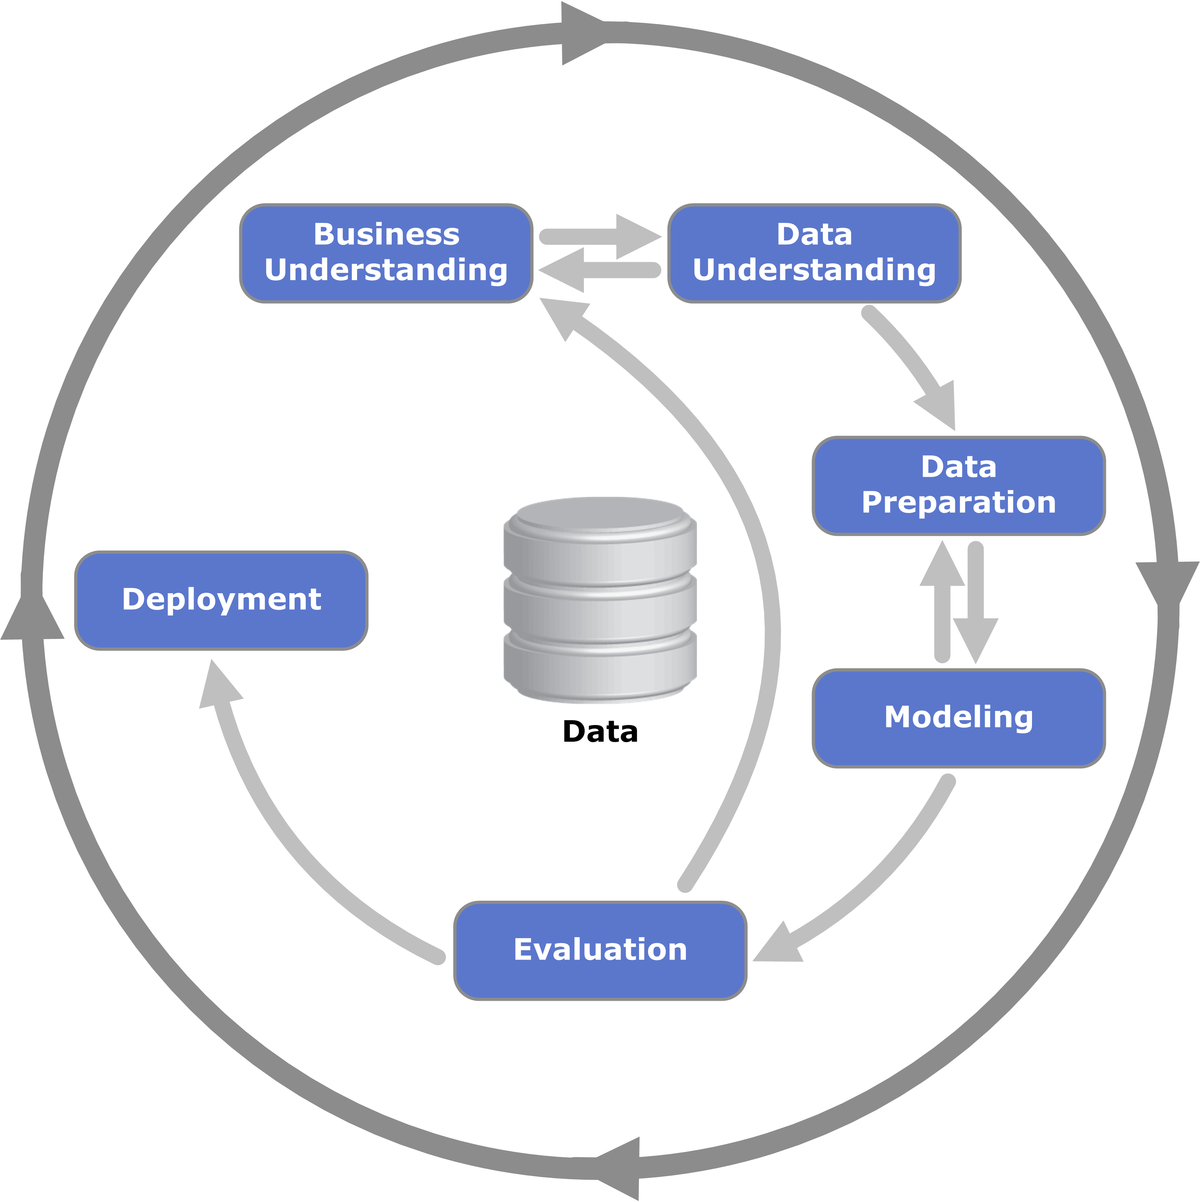
\includegraphics[width=0.35\textwidth]{crispdm.png} % Ajusta el tamaño con width o height
		\caption{Metodología CRISP-DM} % Texto del caption
		\label{fig:crispdm} % Etiqueta para referenciar la imagen
	\end{figure}
	
	
	El método CRISP-DM (Cross Industry Standard Process for Data Mining) se aplicó de la siguiente manera en el desarrollo de este proyecto de minería de textos:
	
	\subsubsection{Comprensión del Negocio}
	Se realizó una revisión exhaustiva del estado del arte, identificando flujos de trabajo y metodologías empleadas en estudios similares, como técnicas de minería de textos, análisis de sentimientos y modelado de tópicos. Con base en estos hallazgos, se diseñó un framework propio adaptado al contexto sociopolítico mexicano. 
	
	\subsubsection{Comprensión de los Datos}
	Se recopilaron dos conjuntos de datos:
	\begin{itemize}
		\item \textbf{YouTube:} Comentarios de los debates presidenciales (9,392 registros), incluyendo atributos como usuario, comentario, canal, número de \textit{me gusta} y fecha.
		\item \textbf{X:} Publicaciones realizadas durante el día de las elecciones (2,486 registros), con atributos como usuario, hora de publicación y contenido textual.
	\end{itemize}
	Se realizó una exploración inicial para identificar datos irrelevantes, valores faltantes y posibles inconsistencias.
	
	\subsubsection{Preparación de los Datos}
	Se implementó un sistema evolutivo de reescritura diseñado para reducir las variantes lingüísticas presentes en los comentarios. Este sistema abordó groserías, faltas de ortografía, jerga mexicana, terminología política y abreviaturas, con el objetivo de unificar términos y estandarizar el texto para su posterior análisis. 	
	
	\subsubsection{Modelado}
	Para el análisis de sentimientos, se utilizó el modelo preentrenado BETO, especializado en español. Este modelo fue ajustado mediante \textit{fine-tuning} con los datos recopilados, adaptándolo al lenguaje manejado en un contexto electoral en redes sociales. 
	
	Para el modelado de tópicos, se emplearon los \textit{embeddings} generados por BETO, y se aplicó reducción de dimensionalidad mediante UMAP (\textit{Aproximación y Proyección Uniforme de Variedades}). Finalmente, se utilizó el algoritmo de agrupamiento HDBSCAN para identificar y clasificar los tópicos principales.
	
	\subsubsection{Evaluación}
	Los resultados del análisis de sentimientos se evaluaron utilizando la matriz de confusión, calculando métricas como precisión y F1-score para cada categoría de sentimiento. Para la evaluación del modelado de tópicos, se utilizó el coeficiente de silueta para medir la cohesión y separación de los clusters generados, asegurando la calidad del agrupamiento.
	
	\subsubsection{Despliegue}
	Los resultados del análisis se presentaron en forma de gráficos y visualizaciones interactivas que muestran:
	\begin{itemize}
		\item Distribución de sentimientos por candidato y plataforma.
		\item Evolución de opiniones durante el proceso electoral.
		\item Comparación entre los temas principales discutidos en YouTube y X.
	\end{itemize}
	Estas visualizaciones permiten una interpretación clara y útil para el público interesado en el análisis político y social.
	
	
	\subsection{Descripción de las Variables del Conjunto de Datos}
	
	A continuación, se presenta la descripción de las variables contenidas en el conjunto de datos:
	\begin{table}[H]
		\centering
		\begin{tabular}{|c|l|p{6cm}|l|p{4cm}|}
			\hline
			\textbf{Núm.} & \textbf{Variable} & \textbf{Significado} & \textbf{Tipo de Dato} & \textbf{Dominio de Valores} \\
			\hline
			1 & \texttt{num\_debate} & Número del debate presidencial en el que se realizó el comentario. & Entero & \{1, 2, 3\} \\
			\hline
			2 & \texttt{canal} & Nombre del canal de YouTube donde se transmitió el debate. & Cadena de texto & Cualquier canal reconocido (e.g., \textit{Milenio}, \textit{Nmás}). \\
			\hline
			3 & \texttt{username} & Nombre de usuario que realizó el comentario en la plataforma. & Cadena de texto & Texto alfanumérico. \\
			\hline
			4 & \texttt{fecha} & Fecha en la que se publicó el comentario. & Fecha & Formato DD/MM/AAAA. \\
			\hline
			5 & \texttt{comentario} & Contenido textual del comentario realizado por el usuario. & Cadena de texto & Cualquier texto. \\
			\hline
			6 & \texttt{num\_likes} & Número de \textit{me gusta} que recibió el comentario. & Entero & \{0, 1, 2, \dots\} \\
			\hline
			
		\end{tabular}
		\caption{Descripción de las variables del conjunto de datos de comentarios en YouTube.}
		\label{tab:variables_dataset}
	\end{table}
	
	\begin{table}[h]
		\centering
		\begin{tabular}{|c|l|p{5cm}|l|p{4cm}|}
			\hline
			\textbf{Núm.} & \textbf{Variable} & \textbf{Significado} & \textbf{Tipo de Dato} & \textbf{Dominio de Valores} \\
			\hline
			1 & \texttt{User} & Nombre del usuario que publicó el tweet. & Cadena de texto & Texto alfanumérico. \\
			\hline
			2 & \texttt{arroba} & Handle del usuario precedido por ``@''. & Cadena de texto & Texto alfanumérico (e.g., \texttt{@usuario}). \\
			\hline
			3 & \texttt{hora\_publicación} & Hora en la que se publicó el tweet. & Hora & Formato HH:MM (24 horas). \\
			\hline
			4 & \texttt{publicación} & Contenido textual del tweet. & Cadena de texto & Texto libre (e.g., comentarios, reacciones). \\
			\hline
		\end{tabular}
		\caption{Descripción de las variables del conjunto de datos de X.}
		\label{tab:variables_dataset_X}
	\end{table}
	
	
	
	\subsection{Tareas de Minería de Datos}
	
	Para realizar el análisis de los comentarios recopilados en redes sociales durante los debates y el día de la elección presidencial, se utilizarán los siguientes algoritmos y técnicas:
	\vspace{-2mm}
	\subsubsection{Análisis del tipo de sentimiento}
	
	El análisis de sentimientos tiene como objetivo clasificar los comentarios en categorías como positivo, negativo y neutral. Para esta tarea se empleará el siguiente enfoque:
	
	\begin{itemize}
		\item \textbf{BETO con Fine-Tuning}: Este modelo preentrenado en español será ajustado mediante \textit{fine-tuning} para capturar patrones textuales específicos del contexto electoral. Este enfoque permite clasificaciones más precisas al considerar dependencias contextuales entre las palabras, adaptándolo al lenguaje y las emociones presentes en las redes sociales.
	\end{itemize}
	
	\vspace{-2mm}
	
	\subsubsection{Análisis de Tópicos}
	
	El análisis de tópicos busca identificar los temas predominantes en los comentarios. Para esta tarea, se implementará una combinación de representaciones de palabras, reducción de dimensionalidad y agrupamiento:
	
	\begin{itemize}
		\item \textbf{Embeddings de Palabras}: Se utilizarán los embeddings de BETO para generar representaciones vectoriales densas de las palabras, capturando relaciones semánticas y contextuales en el corpus de texto.
		\item \textbf{Reducción de Dimensionalidad con UMAP}: Antes de aplicar el agrupamiento, se utilizará la Proyección y Aproximación Uniforme de Colectores (UMAP, por sus siglas en inglés) para reducir la dimensionalidad de los embeddings generados, conservando las características más relevantes y mejorando la eficiencia del algoritmo.
		\item \textbf{HDBSCAN}: Sobre los embeddings reducidos, se aplicará el algoritmo de agrupamiento HDBSCAN para identificar grupos de comentarios relacionados con tópicos similares.
	\end{itemize}
	
	
	\subsection{Modelo del Framework de Desarrollo}
	
	\begin{figure}[H] % 'h!' posiciona la imagen cerca del texto relacionado
		\centering
		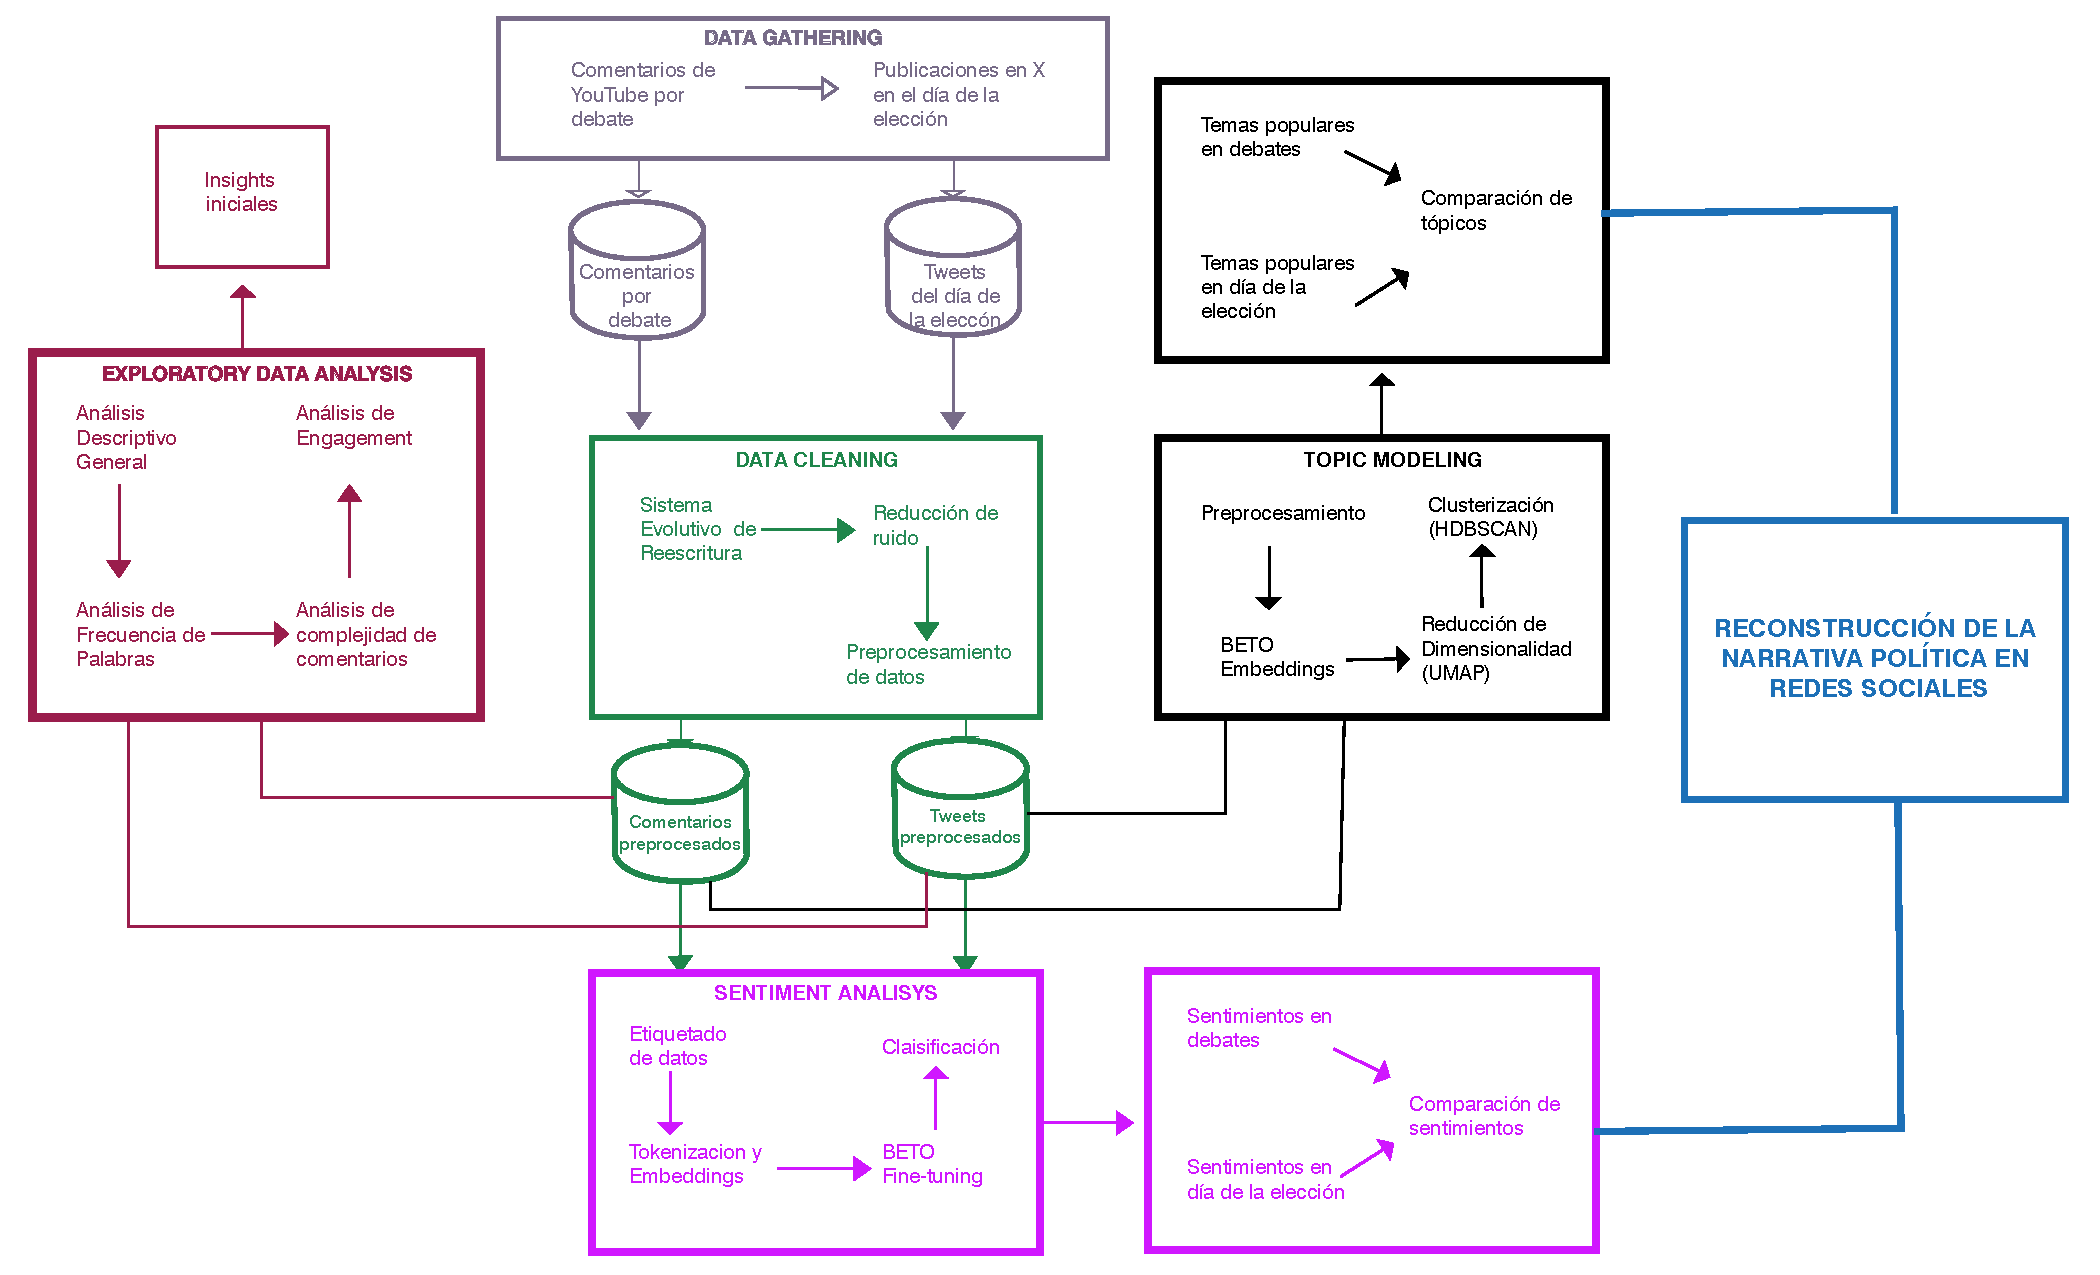
\includegraphics[width=0.73\textwidth]{diagrama.pdf} % Ajusta el tamaño con width o height
		\caption{Framework de Desarrollo} % Texto del caption
		\label{fig:framework} % Etiqueta para referenciar la imagen
	\end{figure}
	
	El presente trabajo propone un framework metodológico para analizar la narrativa política expresada en redes sociales durante las elecciones presidenciales de México 2024. Este marco conceptual combina técnicas de minería de textos, análisis exploratorio de datos, modelado de tópicos y análisis de sentimientos, con el objetivo de proporcionar una comprensión integral sobre la opinión pública y sus dinámicas en contextos digitales.
	
	
	\subsubsection{Recolección de Datos (Data Gathering)}
	El proceso inicia con la recopilación de dos conjuntos de datos principales: comentarios de YouTube publicados durante los debates presidenciales y tweets publicados en la plataforma X el día de la elección. Este paso permite capturar momentos clave del proceso electoral y recopilar un volumen significativo de datos no estructurados.
	
	\subsubsection{Limpieza de Datos (Data Cleaning)}
	Antes de cualquier análisis, los datos son procesados mediante un sistema evolutivo de reescritura, diseñado para reducir el ruido lingüístico, normalizar términos y eliminar ambigüedades semánticas. Este preprocesamiento asegura que los textos estén listos para las siguientes etapas del análisis, preservando la calidad y relevancia de la información.
	
	\subsubsection{Análisis Exploratorio de Datos (Exploratory Data Analysis)}
	Esta etapa se enfoca en extraer \textit{insights} iniciales a través de análisis descriptivos. Incluye estudios sobre la frecuencia de palabras clave, la complejidad de los comentarios y el nivel de interacción o \textit{engagement} observado en las plataformas. Estos análisis permiten identificar patrones generales en los datos.
	
	\subsubsection{Modelado de Tópicos (Topic Modeling)}
	Para descubrir los temas más discutidos en las redes sociales, se aplica una combinación de reducción de dimensionalidad (UMAP) y técnicas de \textit{clustering} (HDBSCAN) utilizando \textit{embeddings} generados por el modelo BETO. Esta etapa facilita la comparación de tópicos entre plataformas y momentos clave, proporcionando un panorama sobre las principales narrativas políticas en los debates y el día de la elección.
	
	\subsubsection{Análisis de Sentimientos (Sentiment Analysis)}
	Los datos preprocesados son clasificados en categorías de sentimiento (positivo, negativo o neutral) mediante un modelo BETO ajustado (\textit{fine-tuning}). Este análisis permite estudiar cómo las emociones del electorado varían entre plataformas y eventos, así como comparar la percepción de los candidatos a lo largo del proceso electoral.
	
	\subsubsection{Reconstrucción de la Narrativa}
	Integrando los hallazgos de las etapas anteriores, el framework busca reconstruir la narrativa política en redes sociales. Esta reconstrucción permite identificar cómo se forman, evolucionan y se difunden las opiniones y emociones del electorado, proporcionando \textit{insights} clave para comprender las dinámicas sociales en entornos digitales.
	
	
	\section{Resultados}
	
	En esta sección se presentará una descripción de los resultados obtenidos en cada una de las etapas descritas en el framework de desarrollo (figura \ref{fig:framework}). De esta manera, se mostrara cómo cada etapa contribuye a generar \textit{insights} sobre las opiniones y temas predominantes expresados durante los debates presidenciales y el día de la elección en las plataformas de redes sociales analizadas.
	
	\subsection{Limpieza de Datos}
	
	Uno de los principales retos al trabajar con datos textuales provenientes de redes sociales es la calidad inconsistente del contenido. En este proyecto, se identificaron varios problemas específicos que complican el análisis automatizado:
	
	\begin{itemize}
		\item \textbf{Mala escritura y faltas de ortografía:} Los comentarios y publicaciones contienen errores ortográficos frecuentes, como palabras mal escritas, omisión de acentos y uso incorrecto de mayúsculas o minúsculas. Estos errores dificultan la tokenización y lematización, al aumentar la variabilidad de las palabras.
		
		\item \textbf{Jerga mexicana y expresiones coloquiales:} Muchos usuarios emplean mexicanismos y modismos propios del contexto cultural, como “chido”, “gacho” o “fifí”. Estas expresiones no están presentes en la mayoría de los diccionarios estándar, lo que limita el desempeño de los modelos preentrenados en el análisis semántico.
		
		\item \textbf{Uso de groserías y lenguaje ofensivo:} Palabras altisonantes como “pendejo” o “culero” son comunes en las discusiones políticas en redes sociales. Estas palabras no solo tienen connotaciones emocionales fuertes, sino que también presentan múltiples variantes (e.g., \textit{pendejo}, \textit{culero}), lo que incrementa la complejidad del análisis de sentimientos.
		
		\item \textbf{Abreviaturas y términos políticos:} Los usuarios utilizan abreviaturas y siglas para referirse a candidatos o partidos, como “AMLO”, “4T” o “PRIAN”. Además, emplean términos únicos del discurso político en México, como “chairos” y “fifís”, que requieren interpretación contextual para su correcta clasificación.
		
	\end{itemize}
	
	Estos problemas no solo dificultan el procesamiento y análisis de los textos, sino que también pueden introducir sesgos en los resultados al interpretar palabras con múltiples variantes o significados según el contexto.
	
	Para abordar estos desafíos, se implementó un \textit{sistema evolutivo de reescritura} \parencite{galindo1991sistemas}, diseñado para realizar una limpieza parcial y estandarización de los textos. 
	
	\subsubsection{Sistema Evolutivo de Reescritura}
	
	Este sistema incluye las siguientes funciones:
	\begin{itemize}
		\item Corrección automática de errores ortográficos y adición de acentos en palabras comunes.
		\item Reducción de variantes de mexicanismos y groserías a una forma estándar.
		\item Reescritura de abreviaturas y siglas, asociándolas con su significado completo en el contexto electoral.
	\end{itemize}
	
	\textbf{Funcionamiento básico}:
	\begin{enumerate}
		\item El sistema compara la entrada con las reglas almacenadas.
		\item Si encuentra una coincidencia, aplica la transformación especificada en la regla.
		\item Si no encuentra una coincidencia, solicita una nueva regla, que luego se añade al sistema.
		\item Este proceso permite que el sistema \textit{aprenda} y mejore con el tiempo, adaptándose a nuevos escenarios y ampliando su base de conocimiento.
	\end{enumerate}
	
	
	Como primer paso para implementar el sistema evolutivo de reescritura, construimos una bolsa inicial de 136 palabras que incluyen términos coloquiales, términos de política mexicana, groserías y abreviaturas comunes en redes sociales. Este conjunto se elaboró a partir de una revisión exhaustiva de los comentarios y publicaciones del conjunto de datos. Algunos ejemplos de palabras incluidas son:
	
	\begin{table}[H]
		\centering
		\resizebox{\textwidth}{!}{%
			\begin{tabular}{|l|c|c|l|l|}
				\hline
				\textbf{Palabra} & \textbf{Nivel de Intensidad} & \textbf{Sentimiento Asociado} & \textbf{Categoría} & \textbf{Comentarios} \\ \hline
				chairo & 3 & negativo & insulto & término despectivo contra votantes de izquierda \\ \hline
				fifi & 3 & negativo & insulto & término usado contra votantes de derecha \\ \hline
				asqueroso & 4 & negativo & adjetivo & término coloquial usado para describir desagrado \\ \hline
				mamón & 3 & negativo & insulto & usado para descalificar \\ \hline
			\end{tabular}%
		}
		\caption{Ejemplo de palabras incluidas en la bolsa inicial.}
		\label{tab:bolsa_palabras}
	\end{table}
	
	
	El propósito de esta bolsa de palabras es servir como base para el sistema evolutivo de reescritura. Este sistema aplica las siguientes acciones sobre los textos:
	\begin{itemize}
		\item \textbf{Estandarización:} Palabras con múltiples variantes (e.g., \textit{fifi}, \textit{fifí}) se reducen a una forma única para minimizar ruido semántico.
		\item \textbf{Limpieza:} Groserías, abreviaturas y errores ortográficos son corregidos, con el fin de mejorar la legibilidad y procesabilidad del texto.
	\end{itemize}
	
	Al utilizar esta bolsa de palabras como referencia inicial, el sistema evolutivo de reescritura es capaz de minimizar el ruido en los textos procesados. Esto facilita que el modelo de lenguaje interprete y analice los datos de manera más efectiva, reduciendo la ambigüedad y los sesgos que pueden surgir debido al uso de jerga o expresiones coloquiales.
	
	El sistema evolutivo no solo se limita a esta bolsa inicial; a través de su diseño, puede adaptarse dinámicamente, incorporando nuevas palabras y reglas según se identifiquen durante el análisis. De esta manera, se garantiza que el texto procesado sea progresivamente más limpio y útil para las etapas posteriores de minería de textos y modelado \parencite{galindo1991sistemas}.
	
	\begin{figure}[h!] % 'h!' posiciona la imagen cerca del texto relacionado
		\centering
		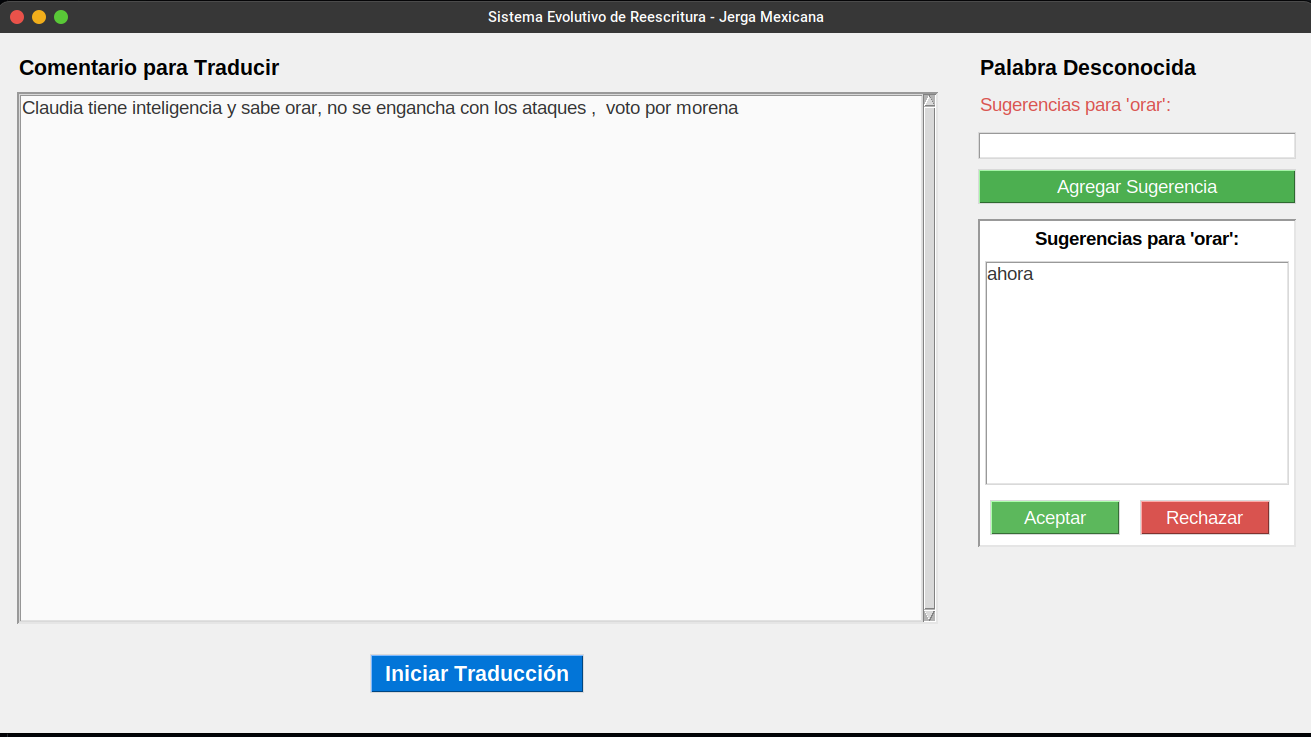
\includegraphics[width=0.7\textwidth]{evolutivo.png} % Ajusta el tamaño con width o height
		\caption{Sistema Evolutivo de Reescritura} % Texto del caption
		\label{fig:evolutivo} % Etiqueta para referenciar la imagen
	\end{figure}
	
	Como resultado de la implementación del sistema evolutivo de reescritura, se logró una reducción del ruido en los textos procesados. Este sistema permitió estandarizar palabras con múltiples variantes, corregir errores ortográficos, reemplazar términos coloquiales, y normalizar abreviaturas utilizadas en el contexto político y social. Tras aplicar este proceso, se generaron versiones actualizadas de los dos conjuntos de datos originales, incorporando una nueva columna denominada \textbf{comentario\_editado}. Esta columna contiene los textos procesados y limpios, listos para ser utilizados en las siguientes etapas de análisis.
	
	\subsubsection{Preprocesamiento de Datos}
	
	Ahora, para continuar con el proceso de minería de textos se aplicó la metodología de preprocesamiento de datos descrita por Gelbukh \parencite{gelbukh2003procesamiento}, que incluye las siguientes etapas fundamentales:
	
	\begin{itemize}
		\item \textbf{Conversión a minúsculas:} Todos los textos fueron convertidos a letras minúsculas para evitar que diferencias de mayúsculas y minúsculas afecten la agrupación de palabras similares.
		
		\item \textbf{Eliminación de emojis y caracteres no textuales:} Se eliminaron los emojis, caracteres especiales y elementos visuales, ya que no aportan información significativa al análisis lingüístico.
		
		\item \textbf{Eliminación de URLs:} Las direcciones web fueron removidas, dado que no representan contenido relevante para el análisis semántico.
		
		\item \textbf{Eliminación de signos de puntuación:} Se eliminaron los signos de puntuación para simplificar la tokenización y garantizar que las palabras sean procesadas sin interferencias.
		
		\item \textbf{Tokenización:} Este proceso consiste en dividir el texto en sus componentes básicos, llamados tokens, que usualmente corresponden a palabras individuales.
		
		\item \textbf{Eliminación de stopwords:} Las palabras vacías, como artículos, preposiciones y conjunciones (por ejemplo, \textit{y}, \textit{de}, \textit{el}), que no aportan significado semántico, fueron eliminadas.
		
		\item \textbf{Lematización:} Cada palabra se redujo a su forma base o lema, eliminando variaciones morfológicas. Por ejemplo, palabras como \textit{comiendo} y \textit{comerán} fueron convertidas a su forma base \textit{comer}.
	\end{itemize}
	
	\subsection{Análisis Exploratorio de Datos}
	
	\subsubsection{Análisis Descriptivo General}
	En esta sección, se presentan las características generales de los datos recopilados, proporcionando una visión inicial de las interacciones en redes sociales relacionadas con los debates presidenciales y el día de la elección en México 2024. Se analizan las distribuciones de comentarios y publicaciones por fecha y hora, así como la frecuencia de menciones a los principales candidatos en las plataformas de YouTube y X.
	
	El análisis exploratorio incluye un conteo de las menciones explícitas a los candidatos Claudia Sheinbaum, Xóchitl Gálvez y Jorge Álvarez Maynez en los comentarios y publicaciones recopilados. Este análisis permite identificar la relevancia de cada candidato en las discusiones y ofrece una perspectiva preliminar sobre las tendencias y temas predominantes en las conversaciones sociales.
		
	\begin{figure}[h!]
		\centering
		\begin{minipage}{0.49\textwidth} % Mitad del ancho de la página
			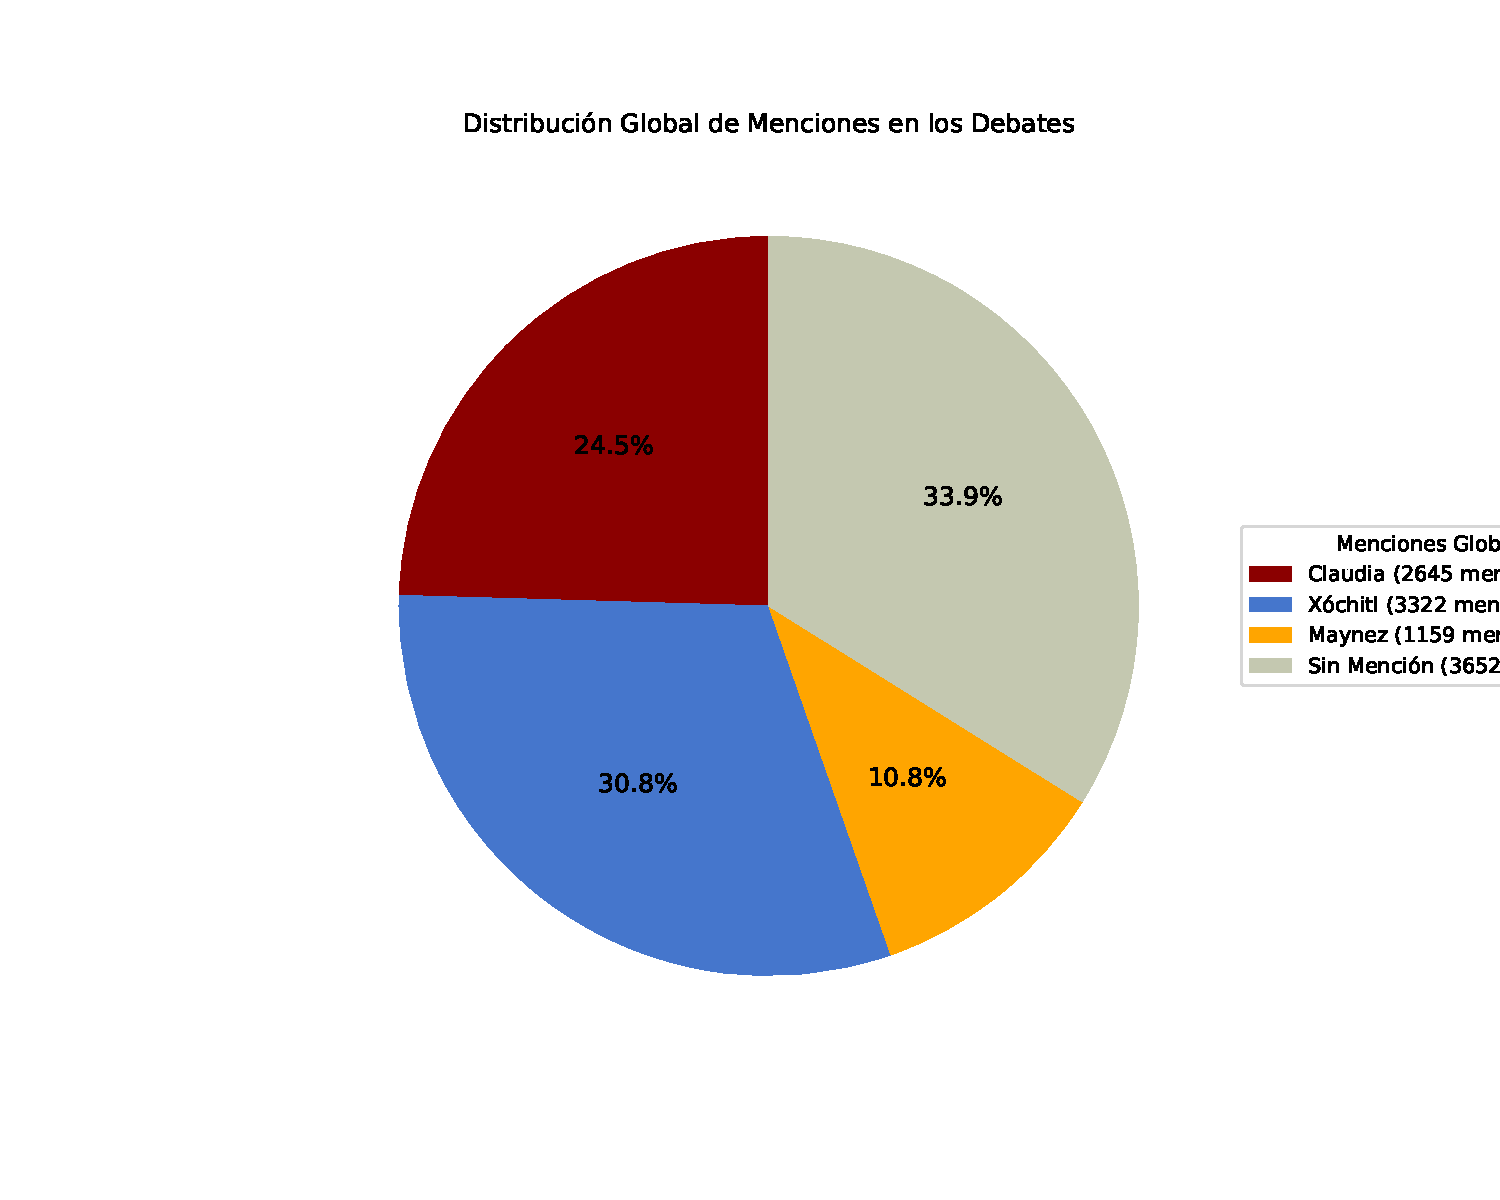
\includegraphics[width=\linewidth]{grafica_global_debates.pdf} 
			\caption{Distribución Global de Menciones en Debates}
			\label{fig:globalDebates}
		\end{minipage}
		\hfill % Espacio flexible entre las dos imágenes
		\begin{minipage}{0.49\textwidth}
			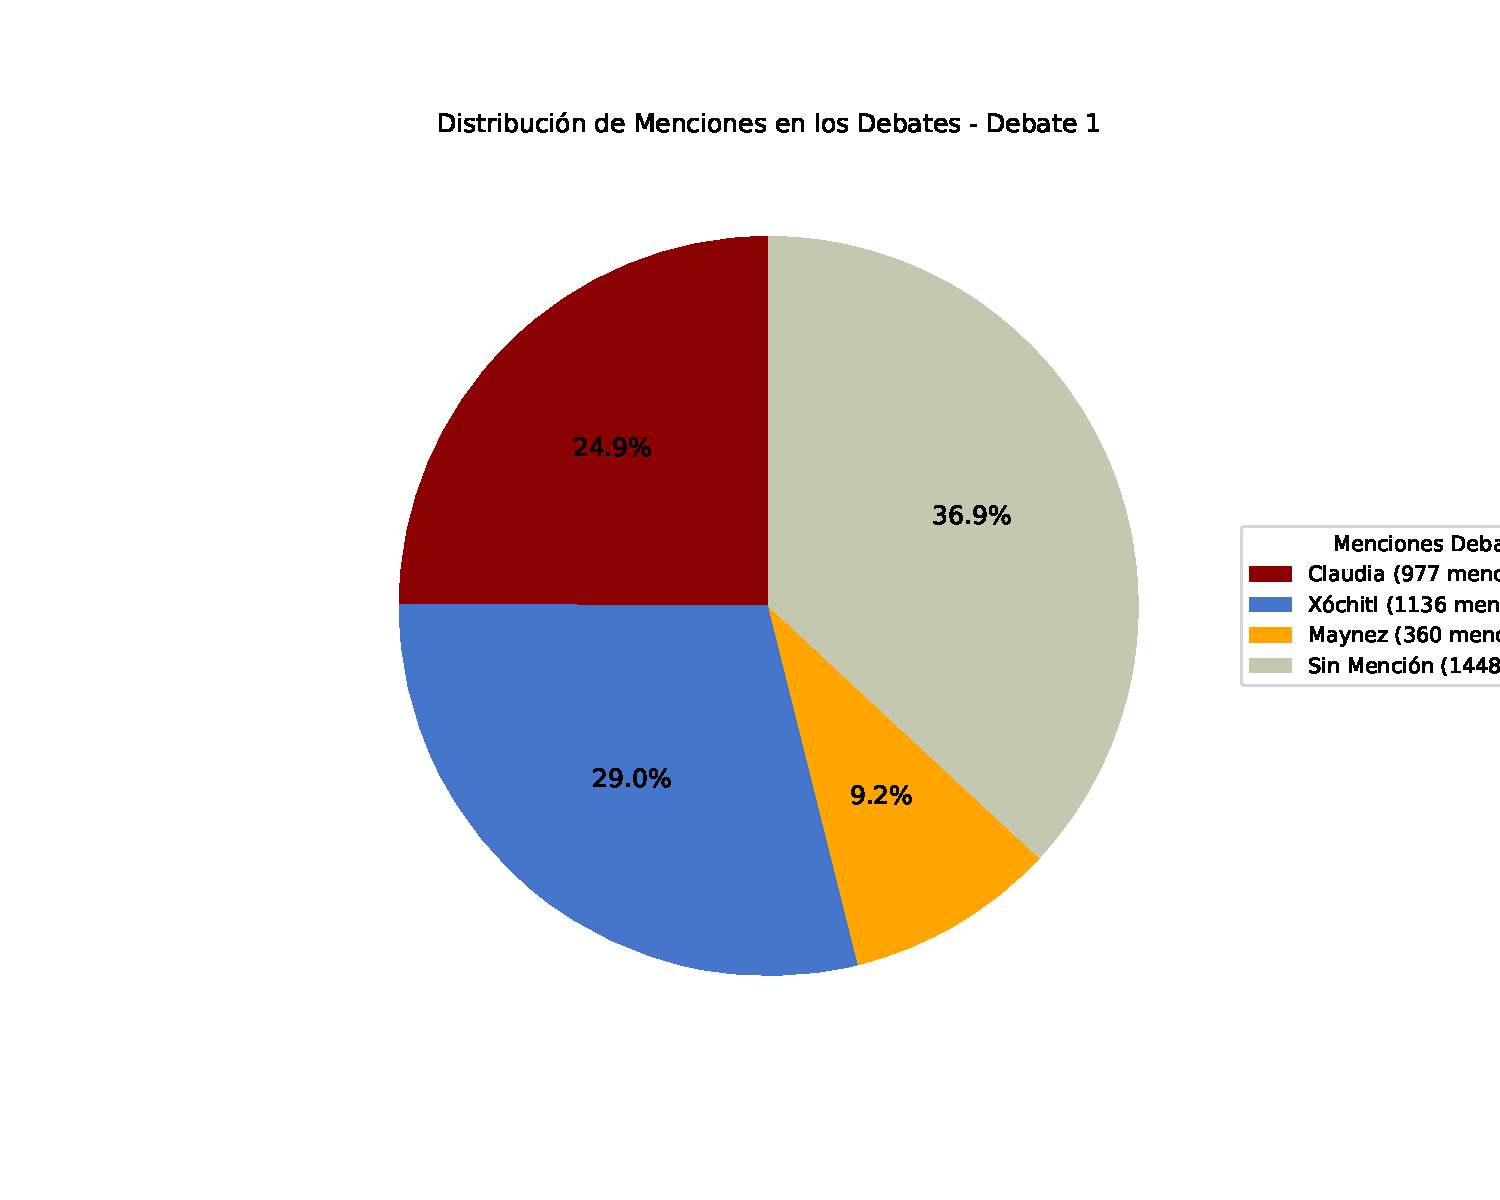
\includegraphics[width=\linewidth]{grafica_debate1.pdf}
			\caption{Distribución en el primer debate}
			\label{fig:distrDebate1}
		\end{minipage}
	\end{figure}
	
	\begin{figure}[h!]
		\centering
		\begin{minipage}{0.49\textwidth} % Mitad del ancho de la página
			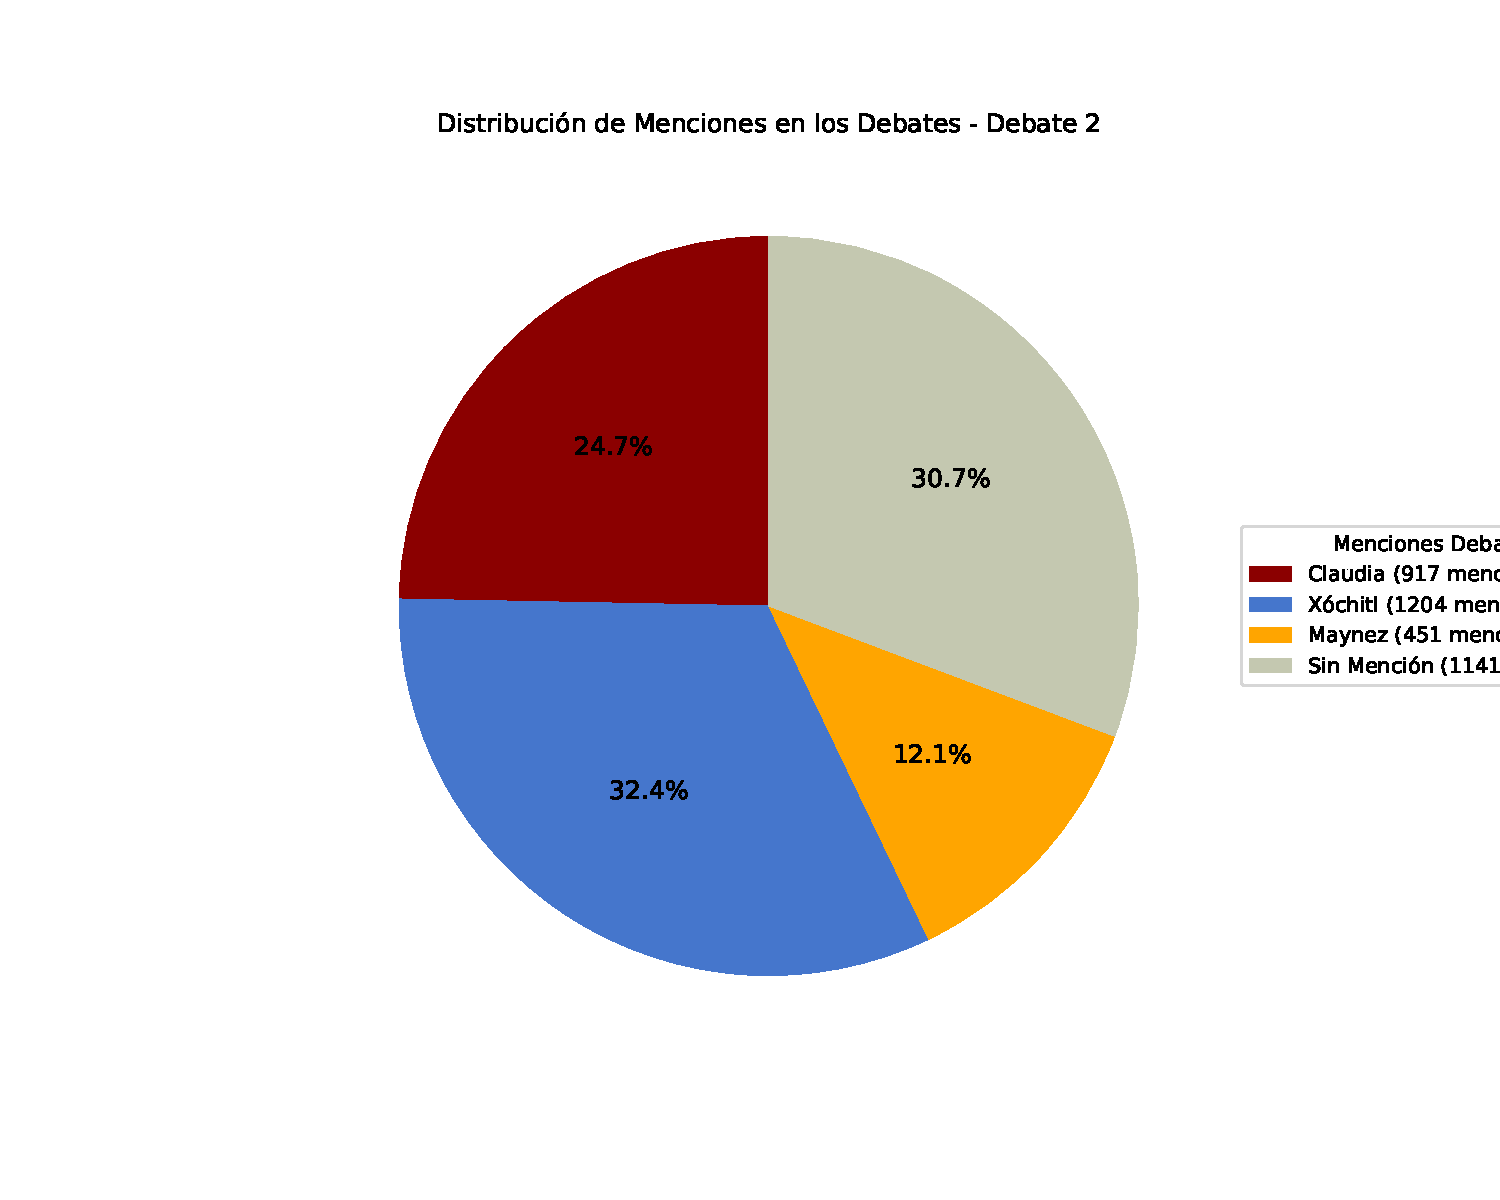
\includegraphics[width=\linewidth]{grafica_debate2.pdf} 
			\caption{Distribución en el segundo debate}
			\label{fig:distrDebate2}
		\end{minipage}
		\hfill % Espacio flexible entre las dos imágenes
		\begin{minipage}{0.49\textwidth}
			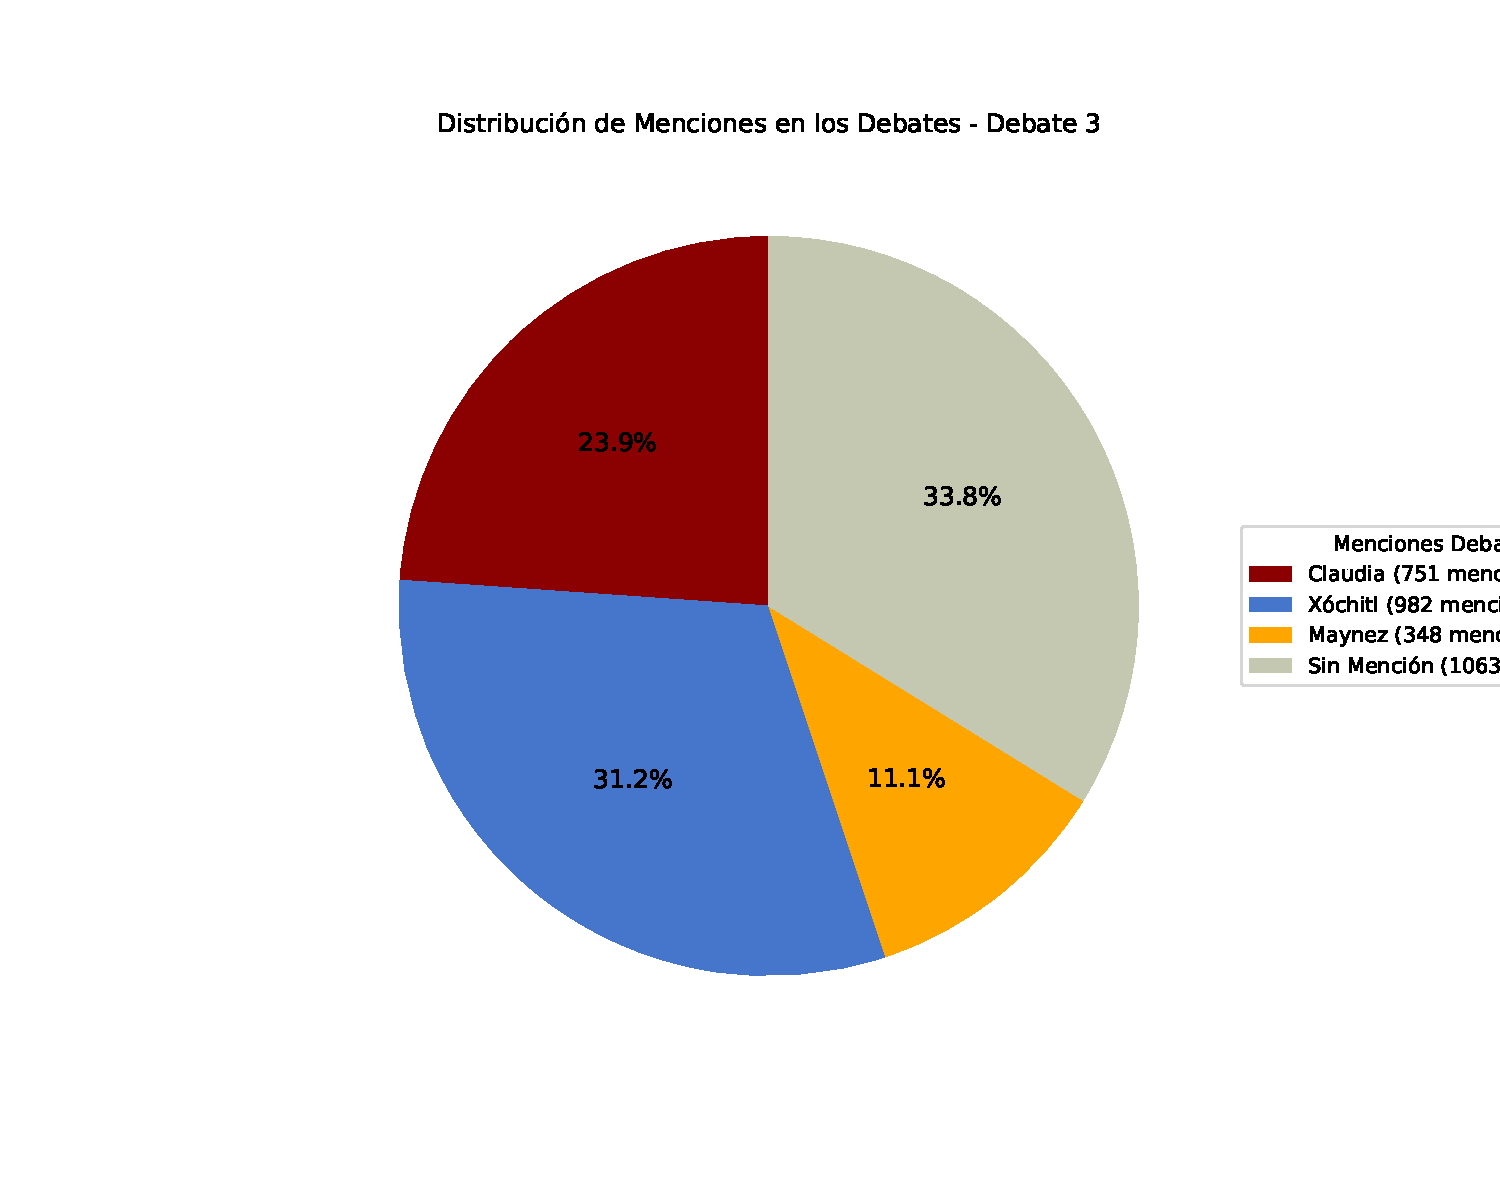
\includegraphics[width=\linewidth]{grafica_debate3.pdf}
			\caption{Distribución en el tercer debate}
			\label{fig:distrDebate3}
		\end{minipage}
	\end{figure}

	
	En el análisis global y por cada debate, se observa una tendencia constante en la distribución de menciones hacia los candidatos:
	
	\begin{itemize}
		\item \textbf{Menciones Generales:} Una proporción considerable de los comentarios no menciona a ningún candidato específico (entre 30\% y 36\% en todas las gráficas). Esto sugiere que una gran parte de las interacciones en los debates se centra en aspectos generales del evento, como la dinámica, los moderadores o los temas tratados, en lugar de los candidatos individuales.
		
		\item \textbf{Competencia entre Claudia y Xóchitl:} Claudia Sheinbaum y Xóchitl Gálvez mantienen una distribución de menciones muy equilibrada en todos los debates, con porcentajes alrededor del 24\% al 32\%. Esto refleja que ambas candidatas generaron un nivel similar de interés y discusión en las redes sociales, consolidándose como las figuras más relevantes del proceso.
		
		\item \textbf{Menor Presencia de Maynez:} Jorge Álvarez Maynez tiene una proporción significativamente menor de menciones, oscilando entre el 9\% y 12\%. Esto sugiere que su participación generó menos resonancia o interés en comparación con las otras dos candidatas.
		
		\item \textbf{Constancia entre los Debates:} Las gráficas muestran una distribución bastante estable a lo largo de los debates, lo que indica que no hubo cambios drásticos en la atención que los usuarios prestaron a cada candidato entre uno y otro evento.
	\end{itemize}

	Para realizar el análisis del día de la elección, se decidió dividir la jornada en intervalos horarios. Este enfoque permitió identificar qué candidato tuvo mayor presencia en las publicaciones realizadas por los usuarios que seguían el desarrollo de la jornada electoral. Tras el procesamiento de los datos, se obtuvieron los siguientes resultados de interacción a lo largo del día.
	
	\begin{figure}[h!]
		\centering
		\begin{minipage}{0.49\textwidth} % Mitad del ancho de la página
			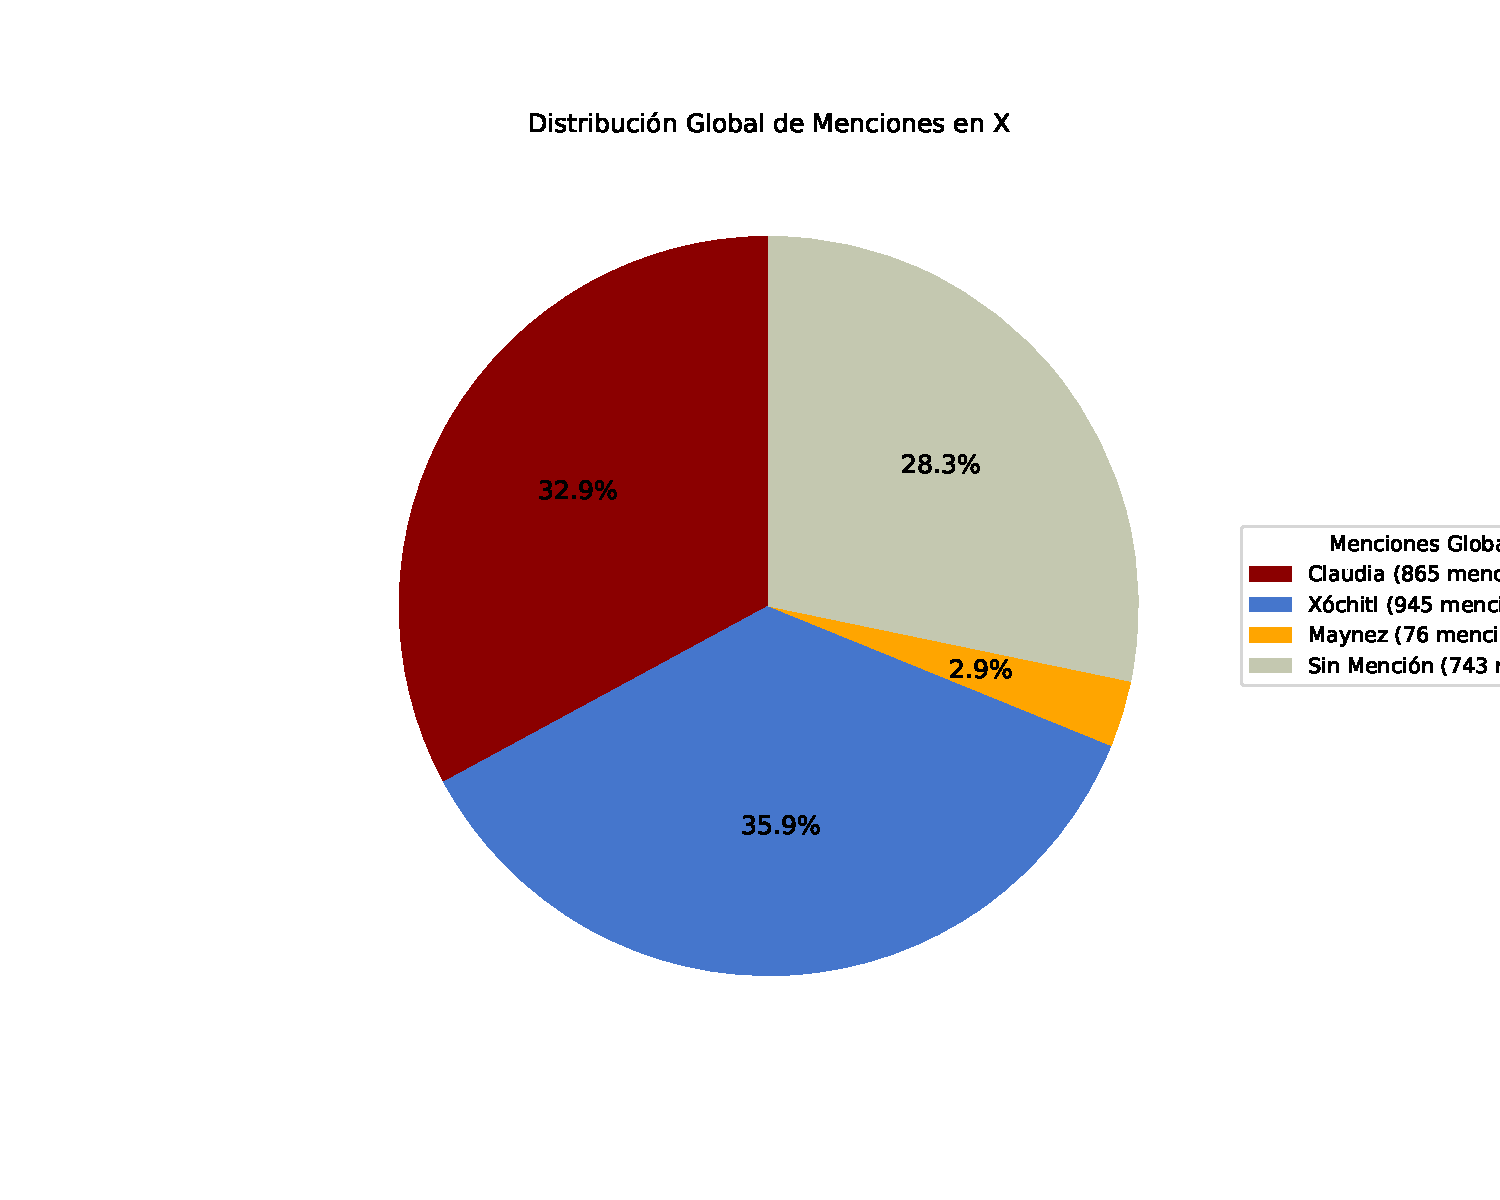
\includegraphics[width=\linewidth]{grafica_global_x.pdf} 
			\vspace{-15mm}
			\caption{Distribución Global de Menciones en el Día de la Elección}
			\label{fig:globalDiaEleccion}
		\end{minipage}
		\hfill % Espacio flexible entre las dos imágenes
		\begin{minipage}{0.49\textwidth}
			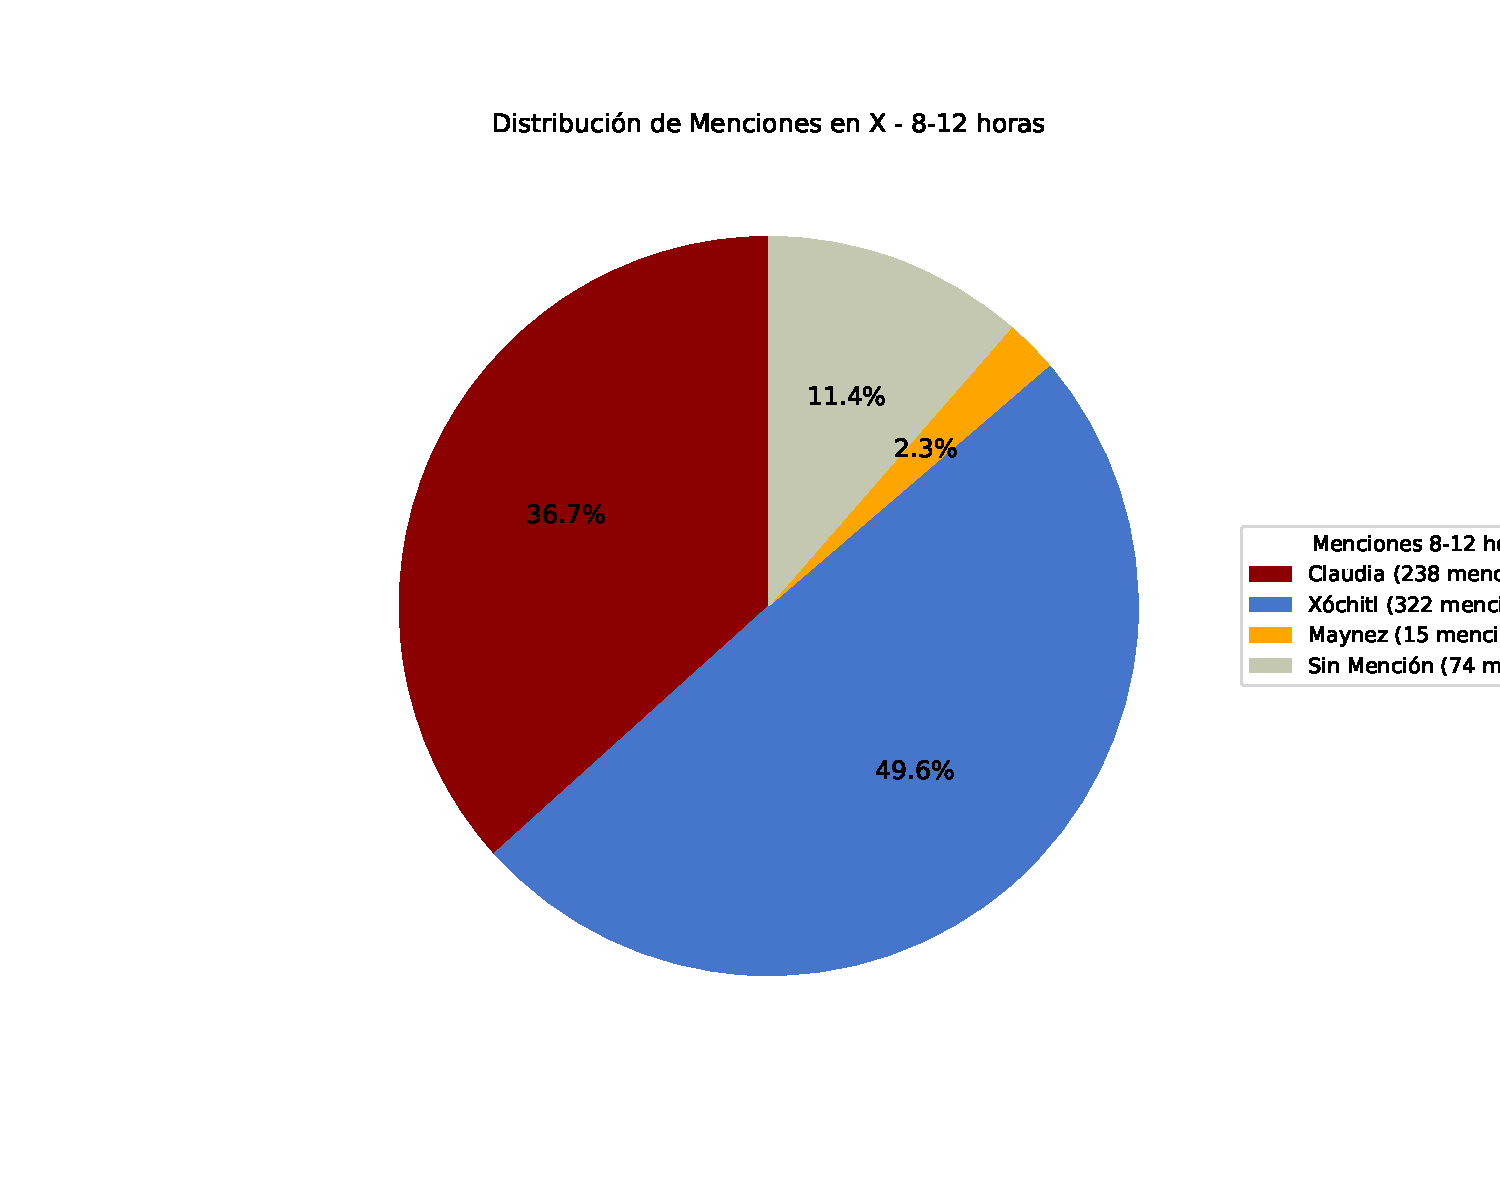
\includegraphics[width=\linewidth]{grafica_intervalo_8-12.pdf}
			\vspace{-15mm}
			\caption{Distribución de Menciones de 08:00 a 12:00}
			\label{fig:xIntervalo812}
		\end{minipage}
	\end{figure}
	
	\begin{figure}[h!]
		\centering
		\begin{minipage}{0.49\textwidth} % Mitad del ancho de la página
			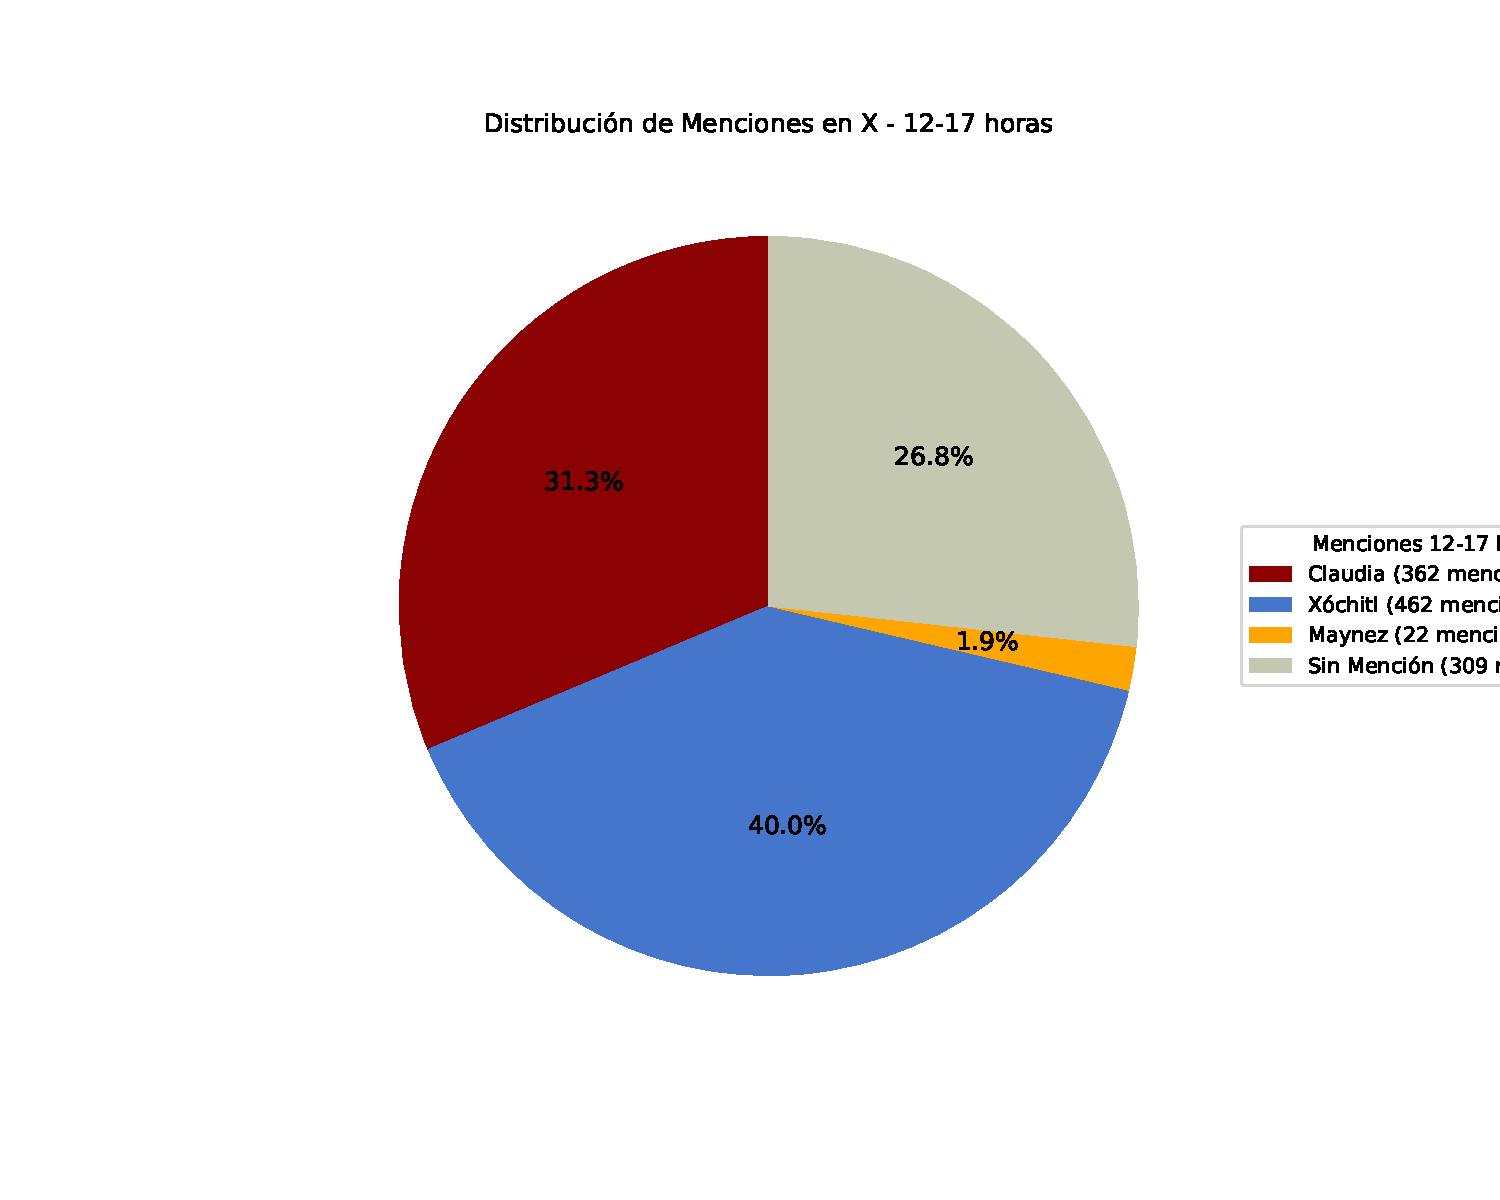
\includegraphics[width=\linewidth]{grafica_intervalo_12-17.pdf} 
			\vspace{-15mm}
			\caption{Distribución de Menciones de 12:00 a 17:00}
			\label{fig:xIntervalo1217}
		\end{minipage}
		\hfill % Espacio flexible entre las dos imágenes
		\begin{minipage}{0.49\textwidth}
			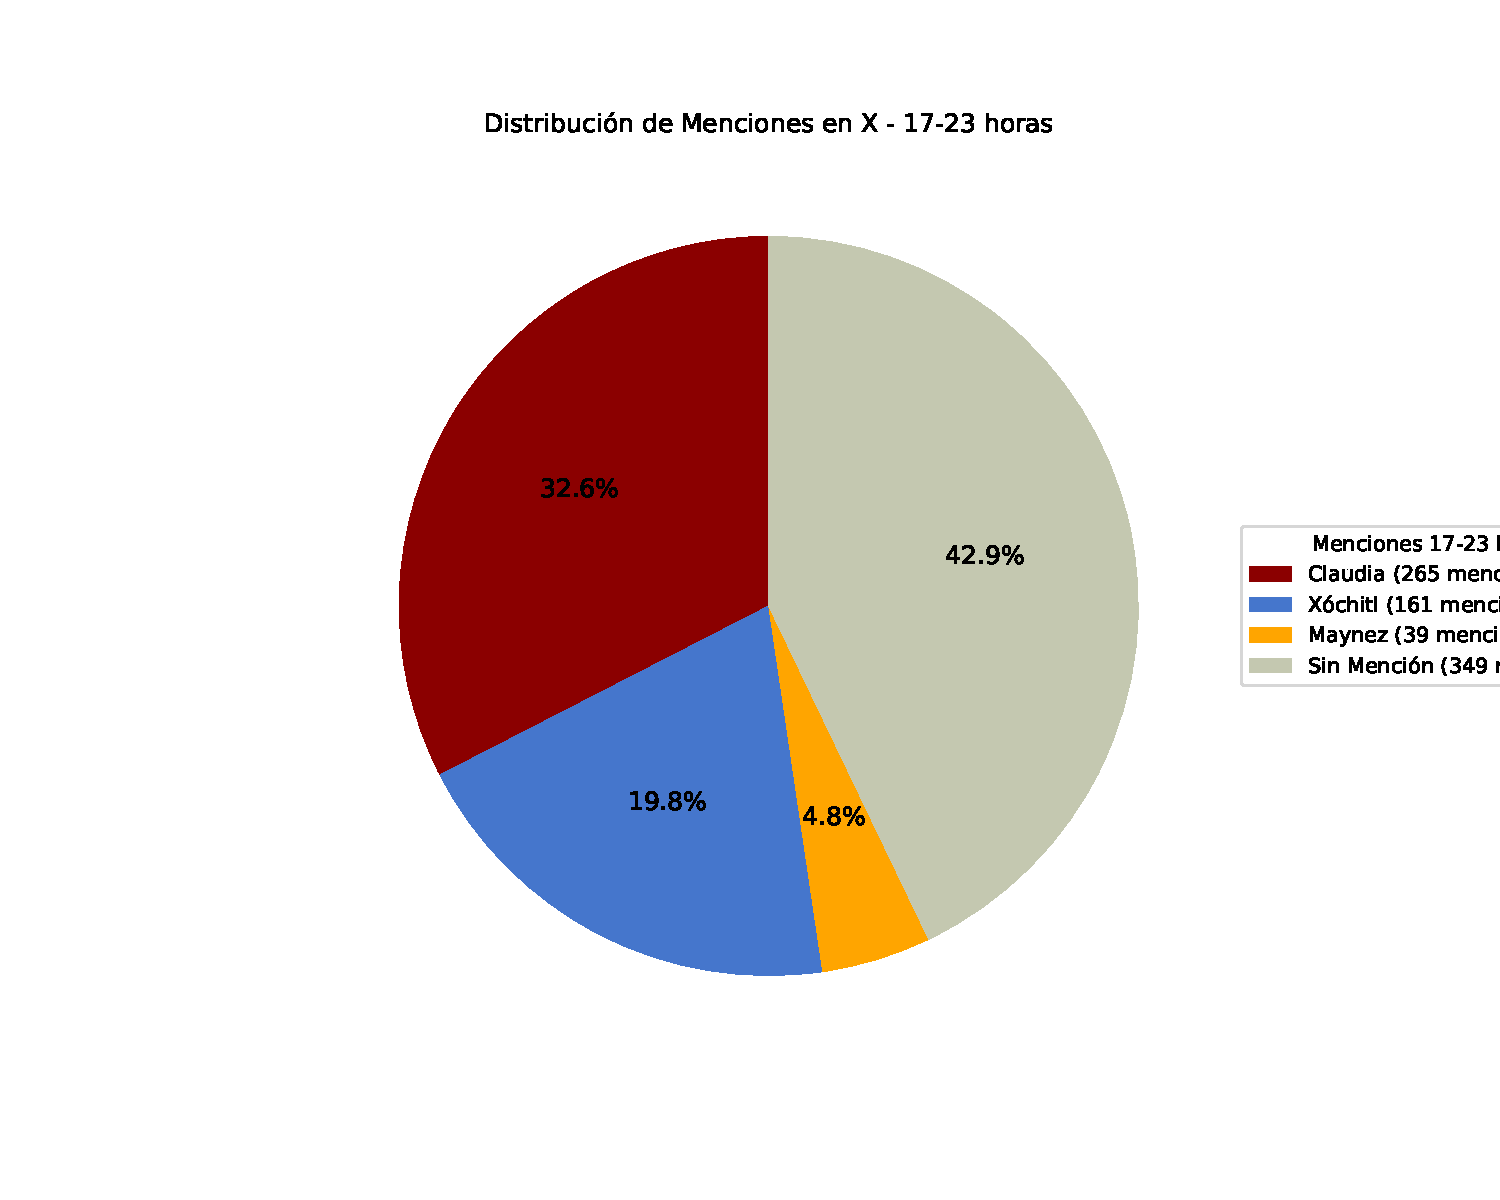
\includegraphics[width=\linewidth]{grafica_intervalo_17-23.pdf}
			\vspace{-15mm}
			\caption{Distribución de Menciones de 17:00 a 23:00}
			\label{fig:xIntervalo1723}
		\end{minipage}
	\end{figure}

	\begin{itemize}
		\item \textbf{Distribución Global:} La proporción de menciones entre Claudia Sheinbaum (32.9\%) y Xóchitl Gálvez (33.9\%) es muy similar, lo que refleja que ambas candidatas generaron un interés equiparable a nivel general. Jorge Álvarez Maynez, con solo el 2.8\% de las menciones, muestra una presencia muy limitada en las discusiones. Los comentarios sin mención específica representan un 30.4\%, lo que sugiere que una parte significativa de las publicaciones aborda temas generales del proceso electoral.
		
		\item \textbf{Intervalo 8-12 horas:} En las primeras horas del día, Xóchitl Gálvez domina con un 47.6\% de las menciones, mientras que Claudia Sheinbaum obtiene el 36.9\%. Jorge Álvarez Maynez tiene un 2.3\%, manteniendo su bajo nivel de atención. Solo el 13.1\% de las publicaciones no menciona candidatos, lo que indica que en este intervalo las discusiones estuvieron más focalizadas en los participantes.
		
		\item \textbf{Intervalo 12-17 horas:} Xóchitl Gálvez sigue liderando con un 39.1\%, aunque su ventaja frente a Claudia Sheinbaum (31.2\%) se reduce Jorge Álvarez Maynez continúa con un bajo porcentaje (1.7\%), lo que evidencia su falta de resonancia durante este intervalo. Las publicaciones sin mención específica aumentan al 27.9\%, lo que podría reflejar una mayor variedad de temas abordados por los usuarios.
		
		\item \textbf{Intervalo 17-23 horas:} Claudia Sheinbaum supera a Xóchitl Gálvez con un 32.7\% frente a 15.9\% de las menciones. Este cambio sugiere que hacia el cierre de la jornada electoral, Claudia captó más atención. Jorge Álvarez Maynez incrementa levemente su porcentaje a 4.6\%, aunque sigue siendo marginal. Las publicaciones sin mención específica alcanzan un 46.8\%, indicando un aumento significativo en los comentarios generales o no relacionados con los candidatos.
	\end{itemize}
	
	
	\subsubsection{Distribución Temporal}
	
	La distribución temporal es importante para identificar patrones y tendencias en la participación de los usuarios en diferentes momentos clave del proceso electoral. Este análisis permite observar cómo varía la cantidad de interacciones a lo largo del tiempo y cómo se concentran en fechas u horarios específicos. En este apartado se analiza la participación en los debates presidenciales y el comportamiento de los usuarios el día de la elección.
	
	\begin{figure}[h!]
		\centering
		\begin{minipage}{0.49\textwidth} % Mitad del ancho de la página
			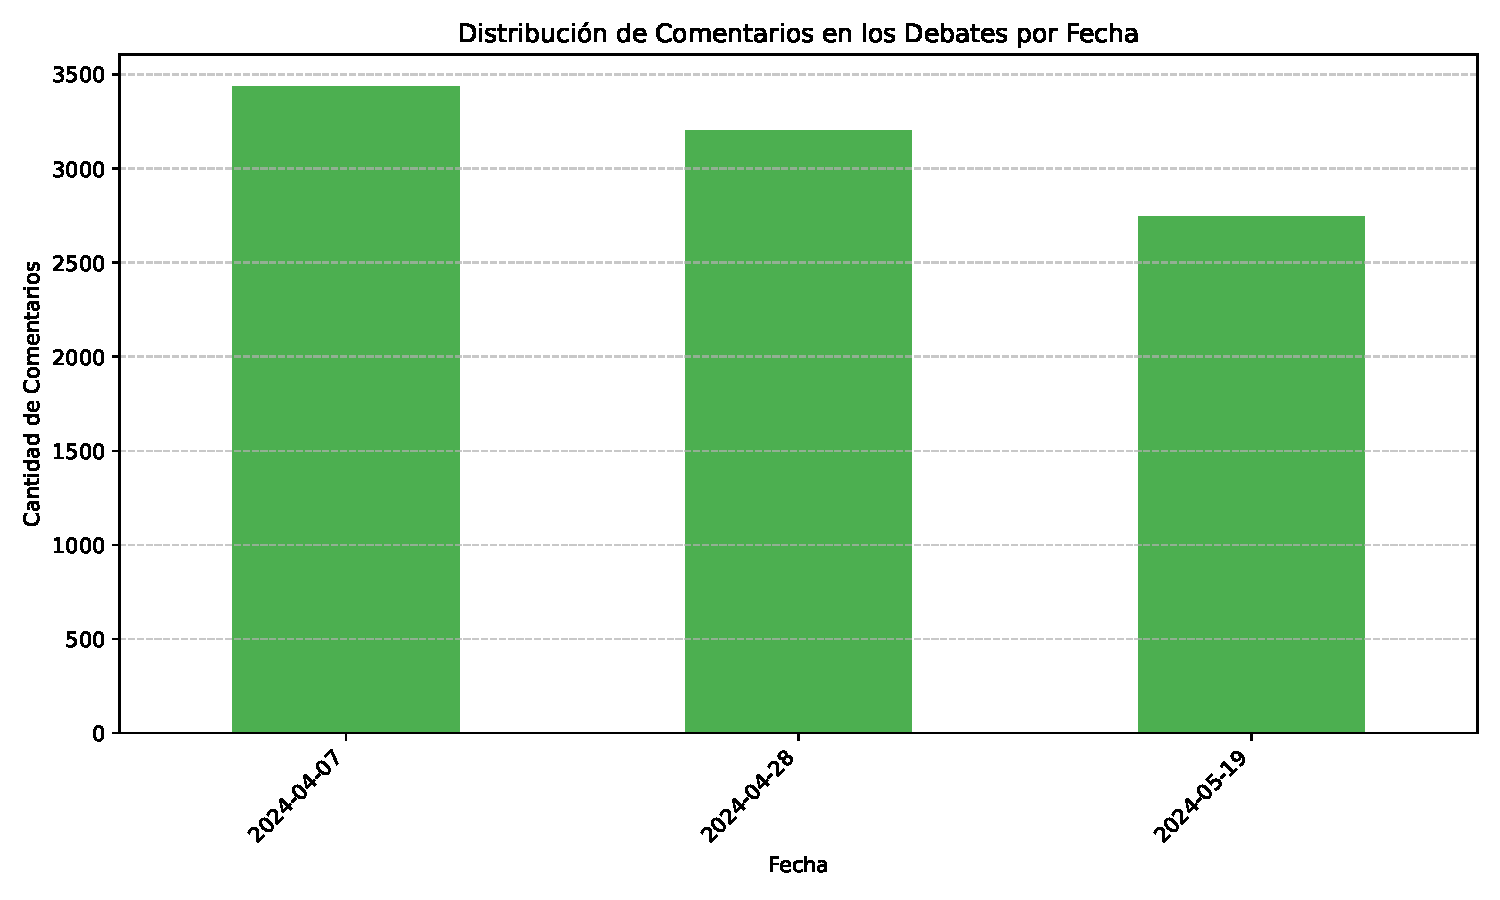
\includegraphics[width=\linewidth]{comentarios_fecha.pdf} 
			\vspace{-5mm}
			\caption{Distribución de Comentarios en los Debates por Fechas}
			\label{fig:temporalDebates}
		\end{minipage}
		\hfill % Espacio flexible entre las dos imágenes
		\begin{minipage}{0.49\textwidth}
			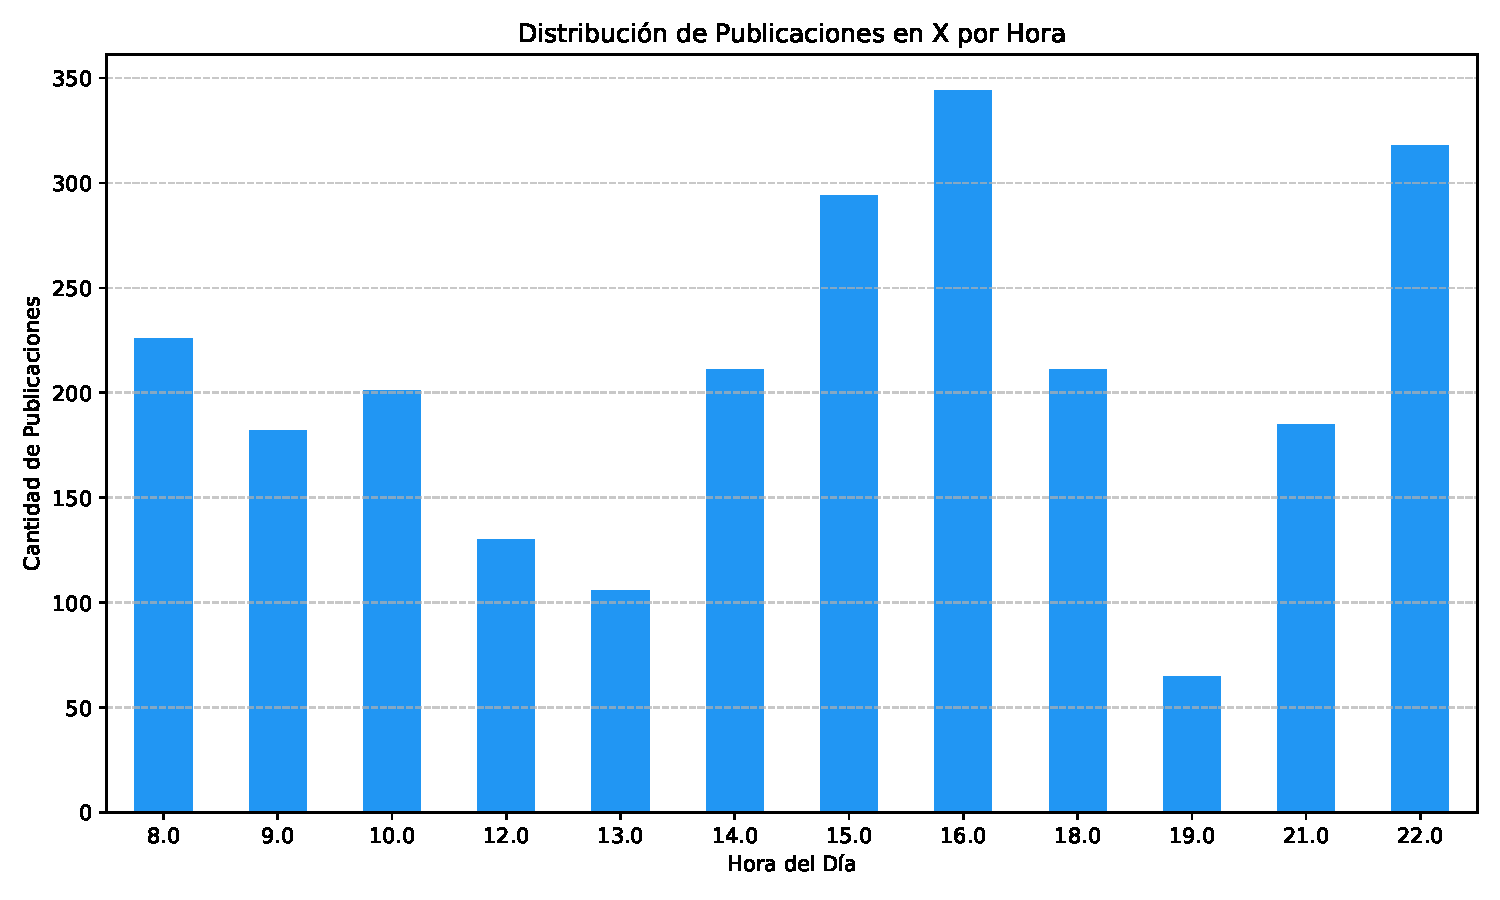
\includegraphics[width=\linewidth]{publicaciones_por_hora.pdf}
			\vspace{-5mm}
			\caption{Distribución de Comentarios en los Debates por Fechas}
			\label{fig:temporalDiaEleccion}
		\end{minipage}
	\end{figure}
	\vspace{-5mm}
	Como se muestra en la figura \ref{fig:temporalDebates}, la gráfica de distribución de comentarios en los debates muestra una participación constante a lo largo de los tres eventos. El debate del 7 de abril de 2024 tuvo el mayor número de comentarios, con un ligero descenso en los debates posteriores, especialmente en el del 19 de mayo de 2024. Esto podría indicar un alto interés inicial en las propuestas de los candidatos, que disminuyó ligeramente hacia el final del ciclo de debates, posiblemente debido a la repetición de ideas o al desgaste del público.
	
	Así también, se observa en la figura \ref{fig:temporalDiaEleccion} que la distribución de publicaciones por hora durante el día de la elección muestra picos claros de actividad a las 16:00 horas y nuevamente a las 22:00 horas, lo que podría reflejar el cierre de las casillas y las discusiones sobre los resultados preliminares. El periodo de menor interacción ocurre alrededor de las 19:00 horas, lo que podría coincidir con un momento de pausa antes del cierre de las votaciones. Esto resalta cómo la actividad en redes sociales está vinculada a hitos clave del día electoral.
	
	
	\subsubsection{Análisis de frecuencias de palabras}
	
	En esta sección se realiza un análisis exploratorio para identificar las palabras más frecuentes en los sets de datos. Se lleva a cabo mediante la generación de nubes de palabras, que permiten visualizar de forma intuitiva los términos más recurrentes en los datos.
	
	\vspace{-4mm}
	\begin{figure}[h!]
		\centering
		\begin{minipage}{0.49\textwidth} % Mitad del ancho de la página
			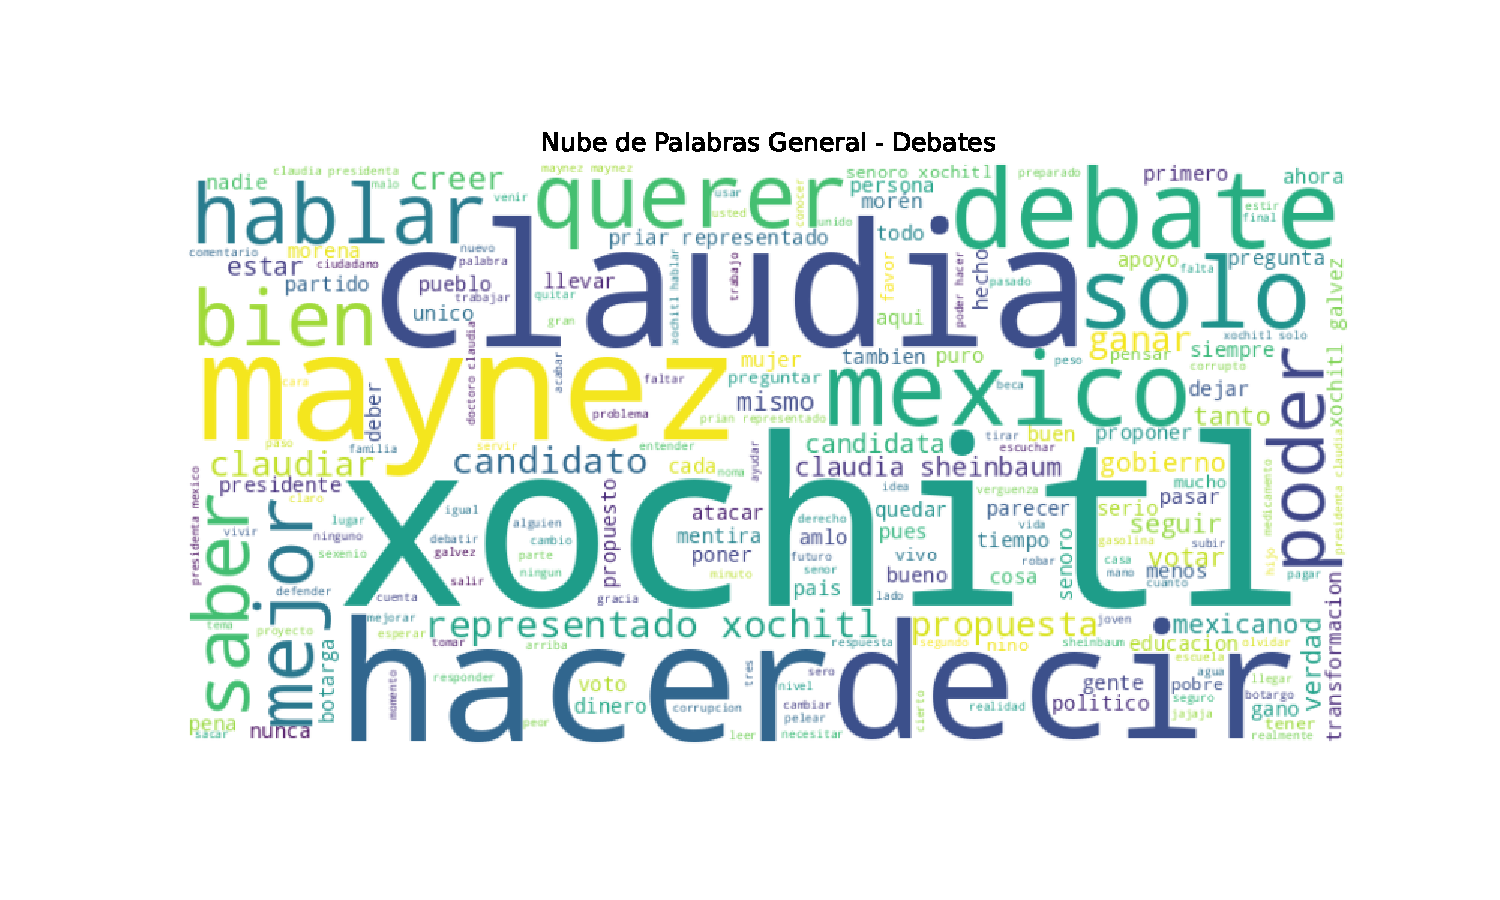
\includegraphics[width=\linewidth]{nube_palabras_general.pdf} 
			\vspace{-10mm}
			\caption{Distribución de Comentarios en los Debates por Fechas}
			\label{fig:Nube de Palabras de los Debates}
		\end{minipage}
		\hfill % Espacio flexible entre las dos imágenes
		\begin{minipage}{0.49\textwidth}
			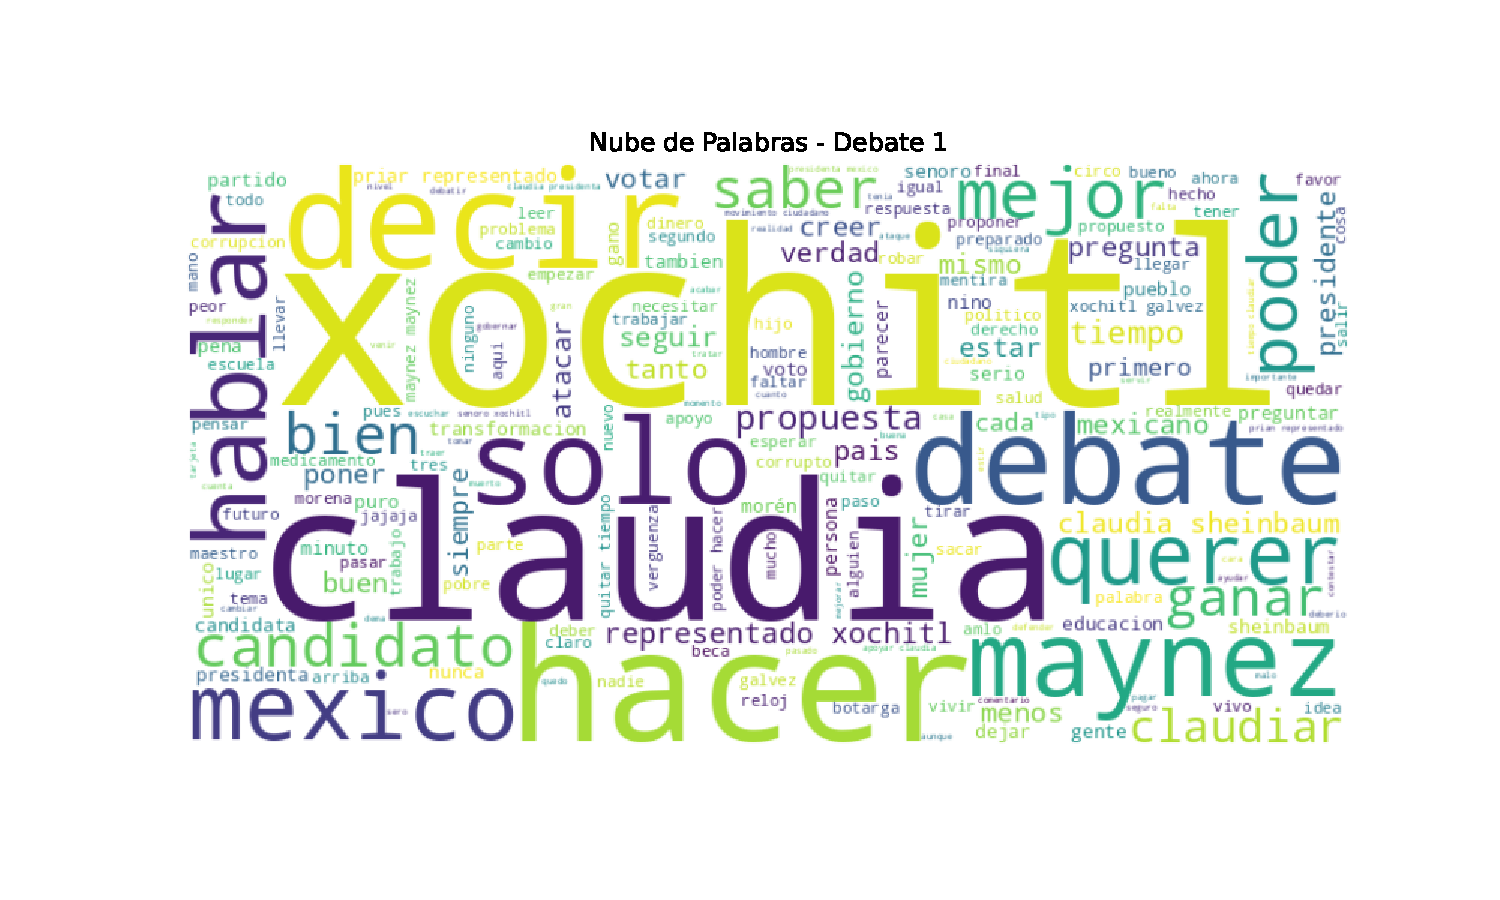
\includegraphics[width=\linewidth]{nube_palabras_debate_1.pdf}
			\vspace{-10mm}
			\caption{Nube de Palabras del Primer Debate}
			\label{fig:nubeDebate1}
		\end{minipage}
	\end{figure}
	
	\vspace{-2mm}
	\begin{figure}[h!]
		\centering
		\begin{minipage}{0.49\textwidth} % Mitad del ancho de la página
			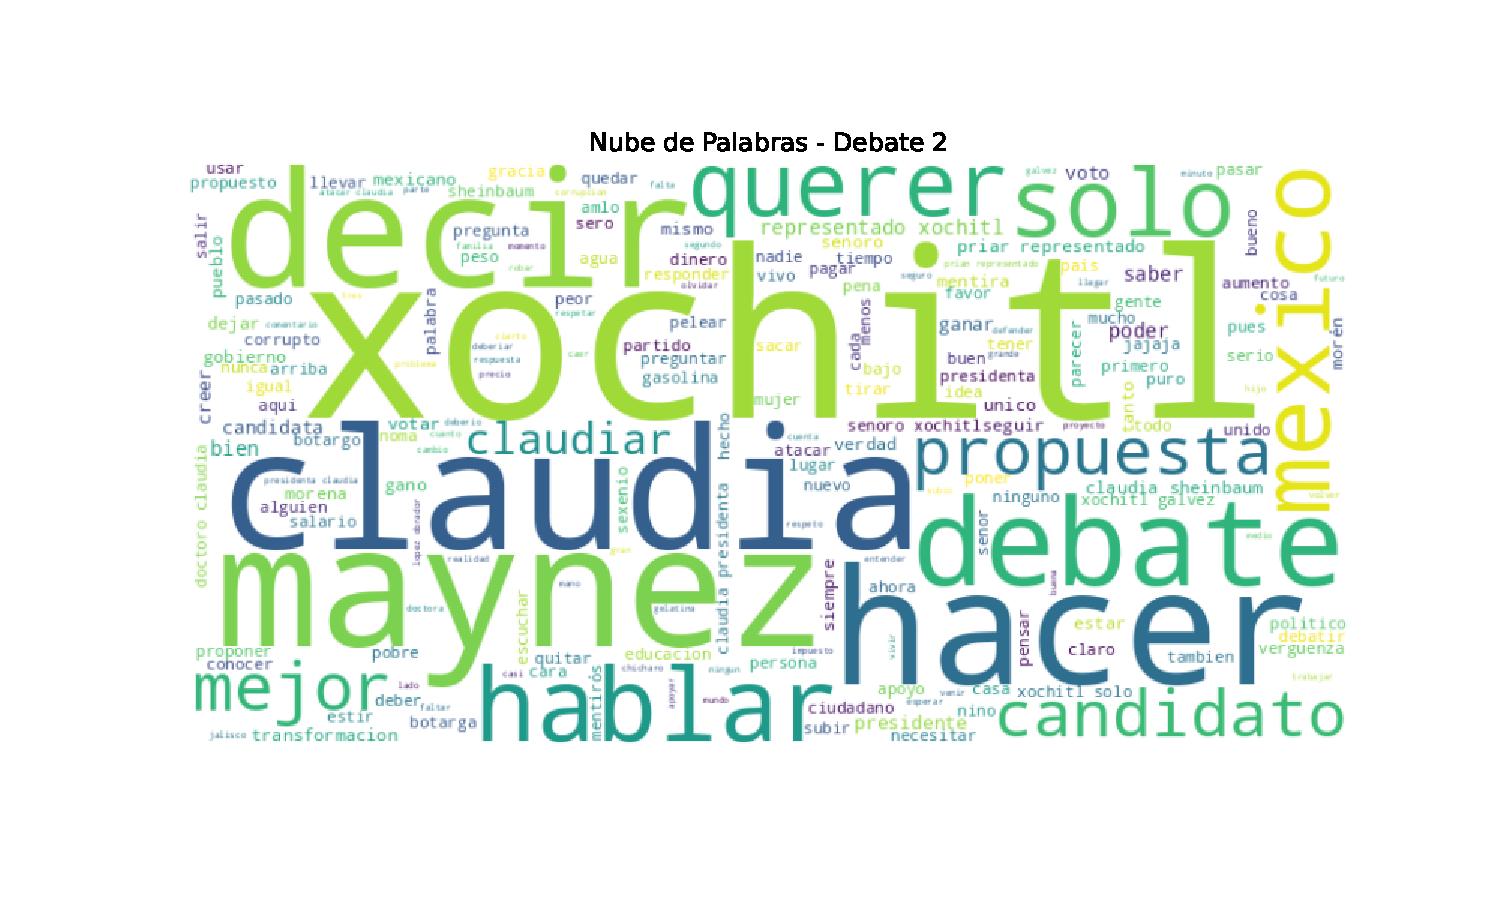
\includegraphics[width=\linewidth]{nube_palabras_debate_2.pdf} 
			\vspace{-10mm}
			\caption{Nube de Palabras del Segundo Debate}
			\label{fig:nubeDebate2}
		\end{minipage}
		\hfill % Espacio flexible entre las dos imágenes
		\begin{minipage}{0.49\textwidth}
			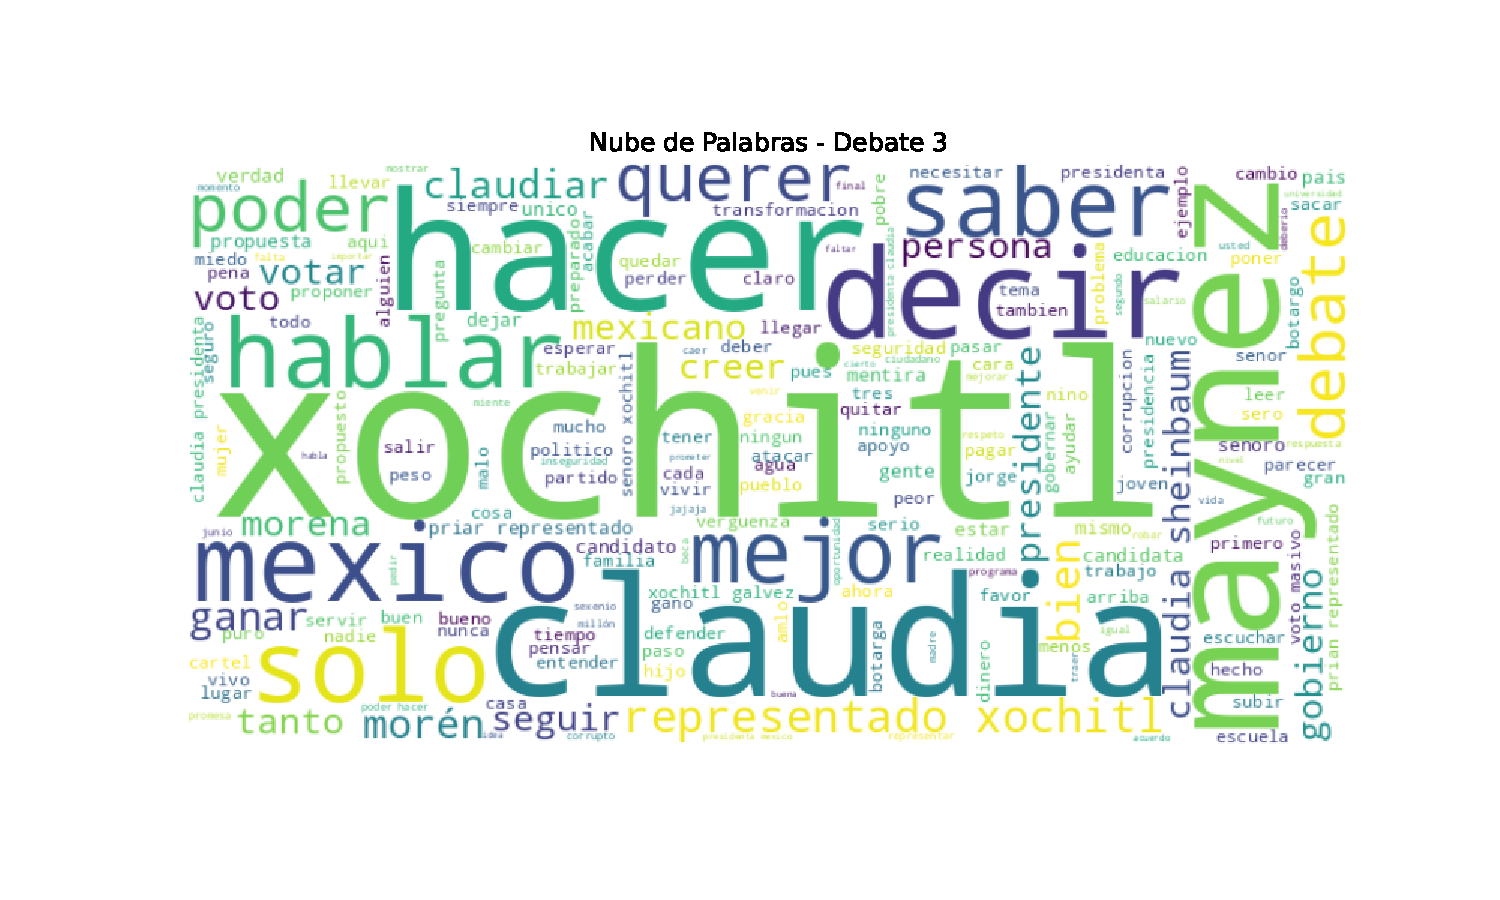
\includegraphics[width=\linewidth]{nube_palabras_debate_3.pdf}
			\vspace{-10mm}
			\caption{Nube de Palabras del Tercer Debate}
			\label{fig:nubeDebate3}
		\end{minipage}
	\end{figure}

	En la nube de palabras general de los debates, se observa una predominancia de términos como \textit{decir, hacer, debate, candidato} y menciones directas a los nombres de los candidatos, como \textit{claudia, xóchitl y maynez}. Esto refleja que las discusiones se centran en las propuestas, el desempeño en los debates y las expectativas de los usuarios en torno a los participantes. Palabras relacionadas con el contexto político y social como \textit{México, gobierno} y \textit{propuesta} también son frecuentes, indicando un interés en los temas tratados.
	
	Por otro lado, en las nubes de palabras individuales de los debates, se observan ligeras variaciones en los términos predominantes. Por ejemplo, en el primer debate destacan términos como \textit{preguntar} y \textit{atacar}, lo que podría sugerir un enfoque más confrontativo. En el segundo debate, términos como \textit{ganar} y \textit{propuesta} son más prominentes, reflejando quizás un tono más propositivo. Finalmente, en el tercer debate, hay una recurrencia de términos como \textit{hablar} y \textit{decir}, sugiriendo un interés en la claridad y el contenido de los mensajes. En conjunto, estas nubes reflejan cómo el enfoque y la percepción de los usuarios varían con el desarrollo de los debates.
	
	Replicando el mismo proceso para el día de la elección y considerando los intervalos definidos anteriormente, podemos observar las nubes descritas a continuación.
	
	\begin{figure}[h!]
		\centering
		\begin{minipage}{0.49\textwidth} % Mitad del ancho de la página
			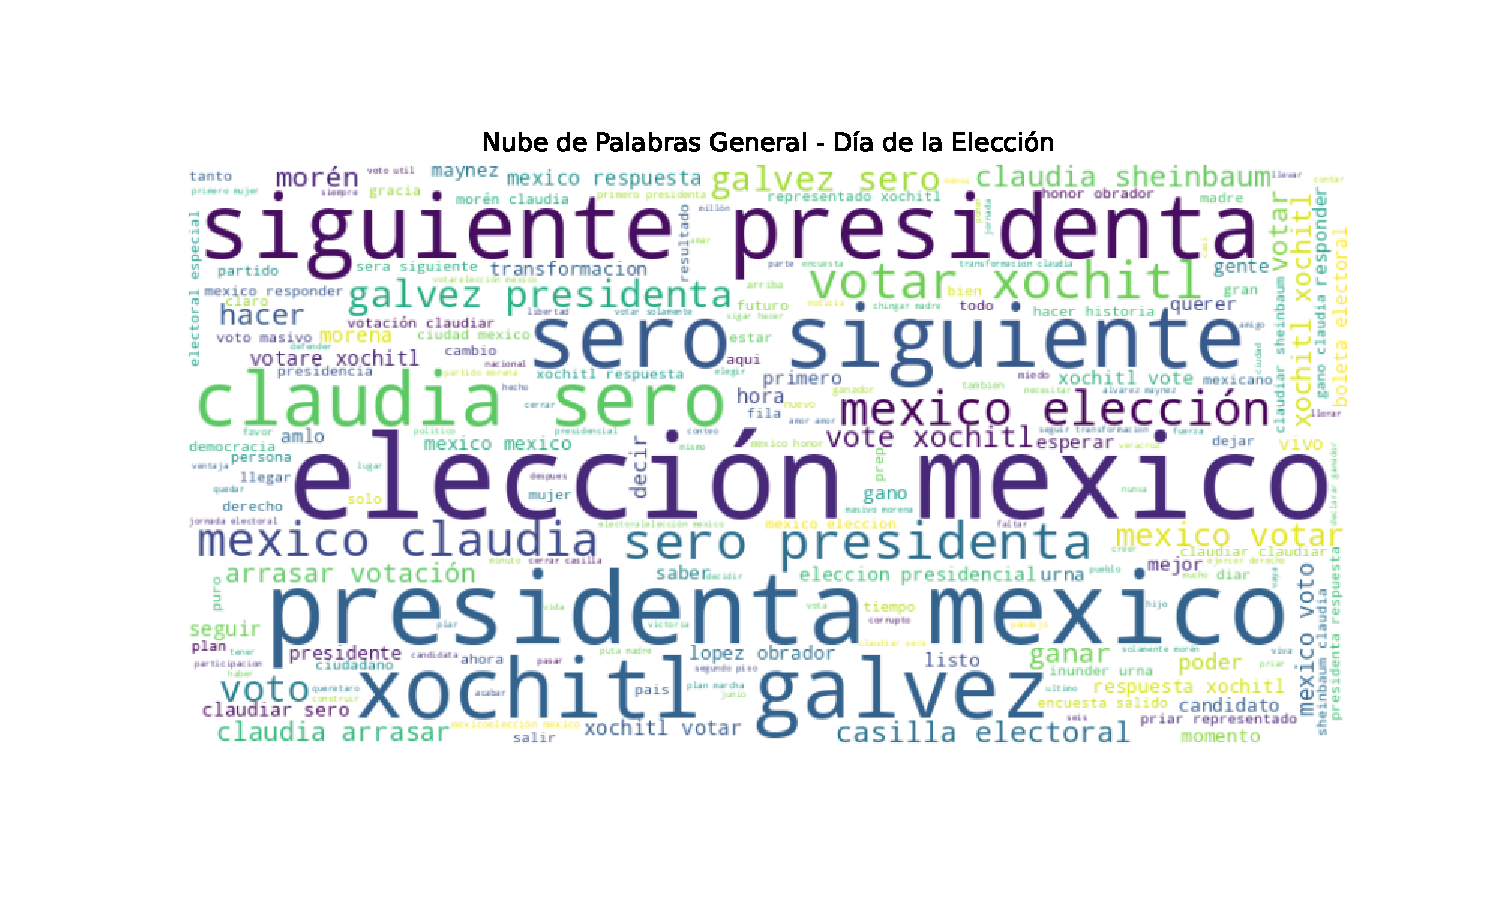
\includegraphics[width=\linewidth]{nube_general_eleccion.pdf} 
			\vspace{-10mm}
			\caption{Nube de Palabras del Día de la Elección}
			\label{fig:nubeDiaEleccion}
		\end{minipage}
		\hfill % Espacio flexible entre las dos imágenes
		\begin{minipage}{0.49\textwidth}
			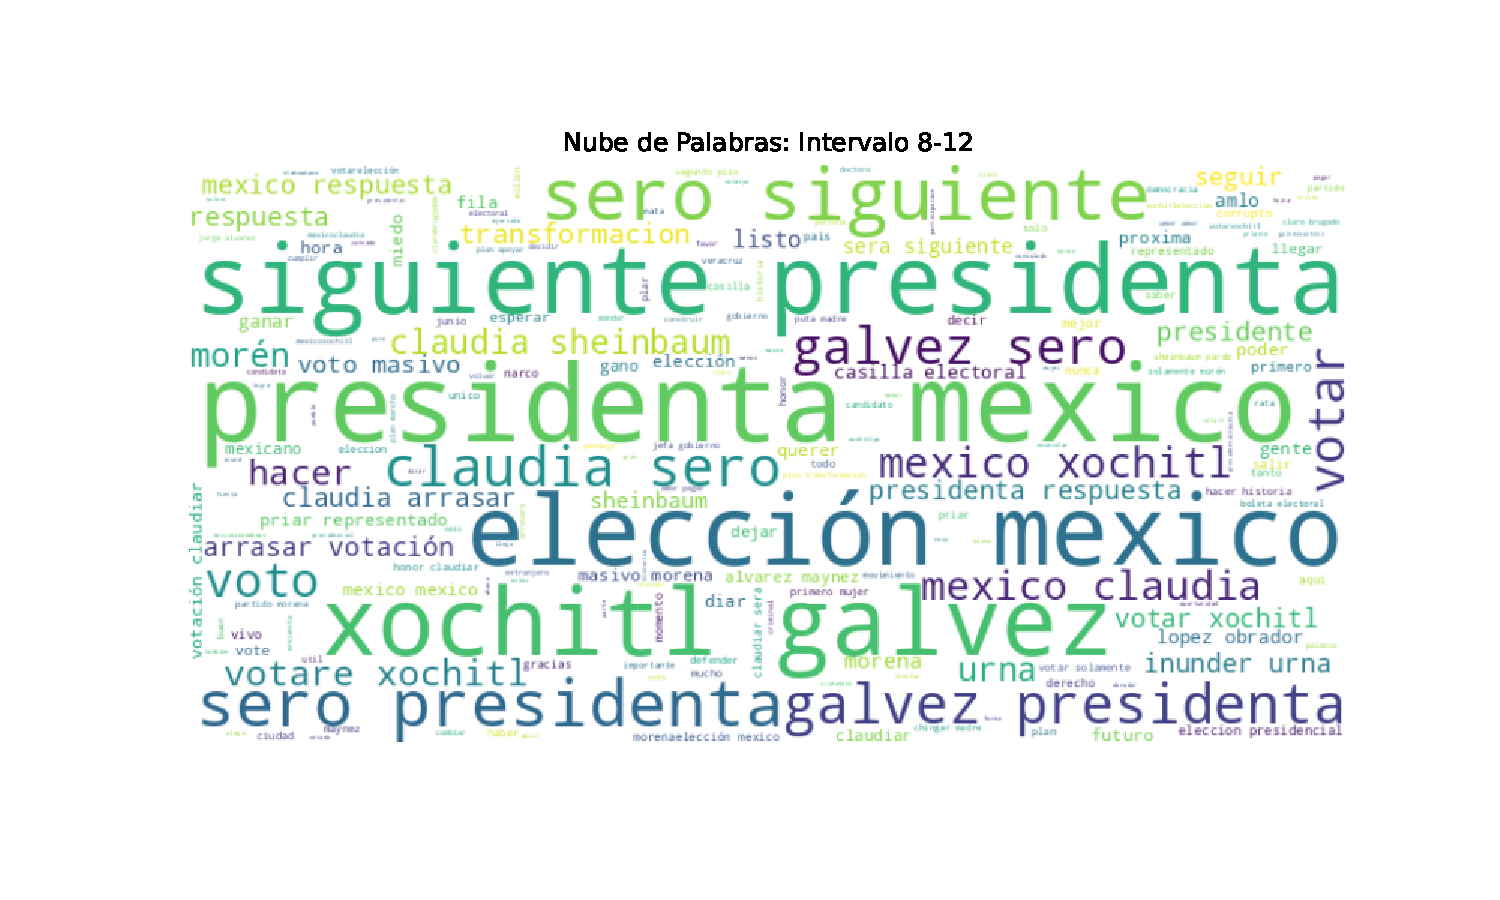
\includegraphics[width=\linewidth]{nube_intervalo_8-12.pdf}
			\vspace{-10mm}
			\caption{Nube de Palabras en el Horario de 08:00 a 12:00}
			\label{fig:nubeIntervalo812}
		\end{minipage}
	\end{figure}
	
	
	\begin{figure}[h!]
		\centering
		\begin{minipage}{0.49\textwidth} % Mitad del ancho de la página
			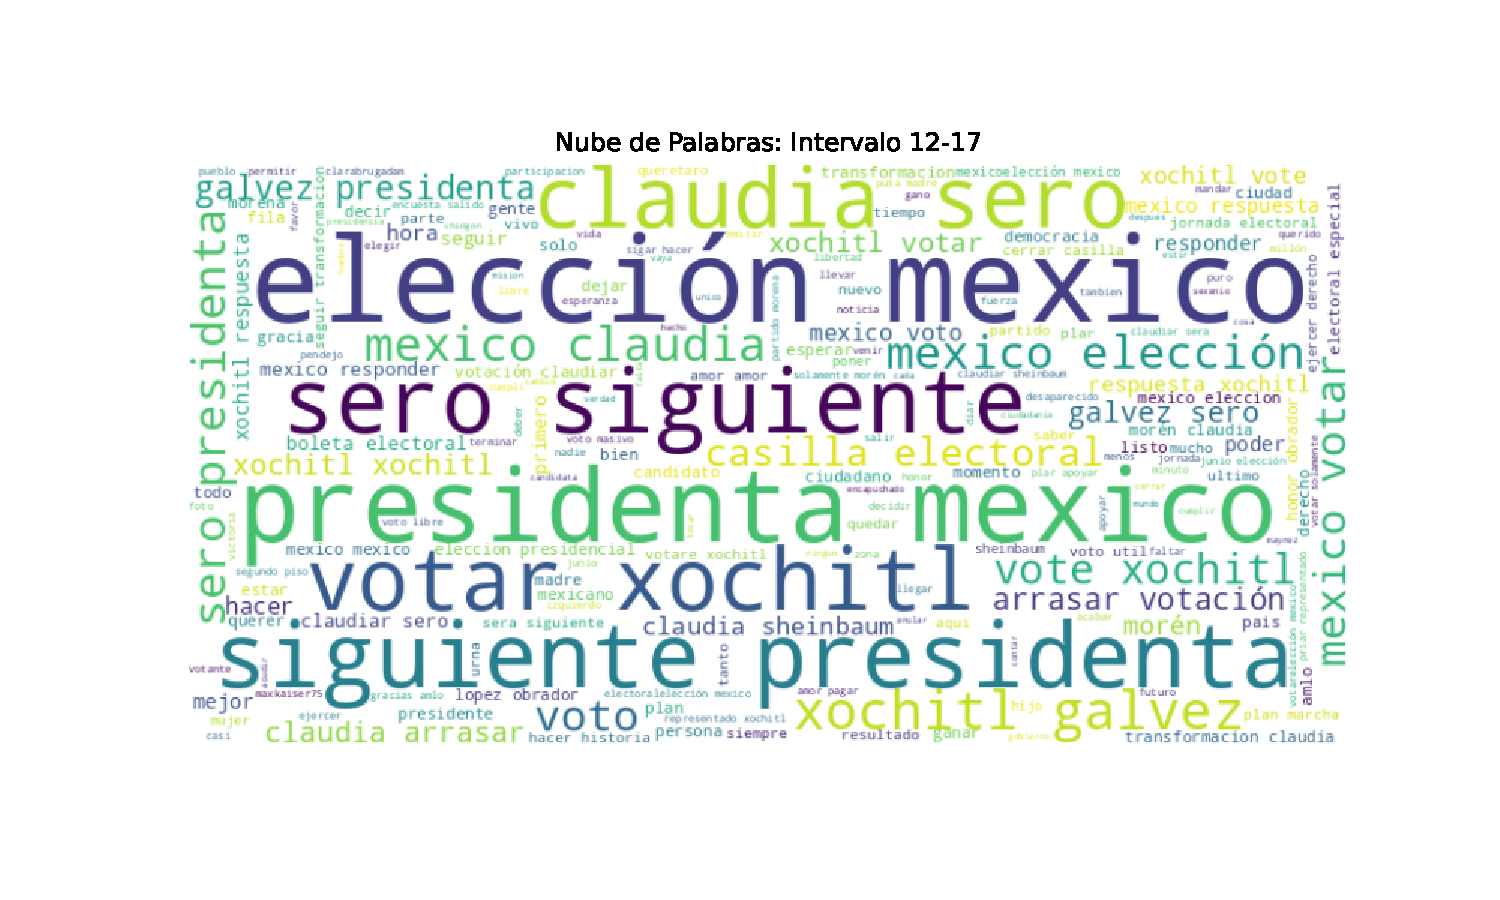
\includegraphics[width=\linewidth]{nube_intervalo_12-17.pdf} 
			\vspace{-10mm}
			\caption{Nube de Palabras en el Horario de 12:00 a 17:00}
			\label{fig:nubeIntervalo1217}
		\end{minipage}
		\hfill % Espacio flexible entre las dos imágenes
		\begin{minipage}{0.49\textwidth}
			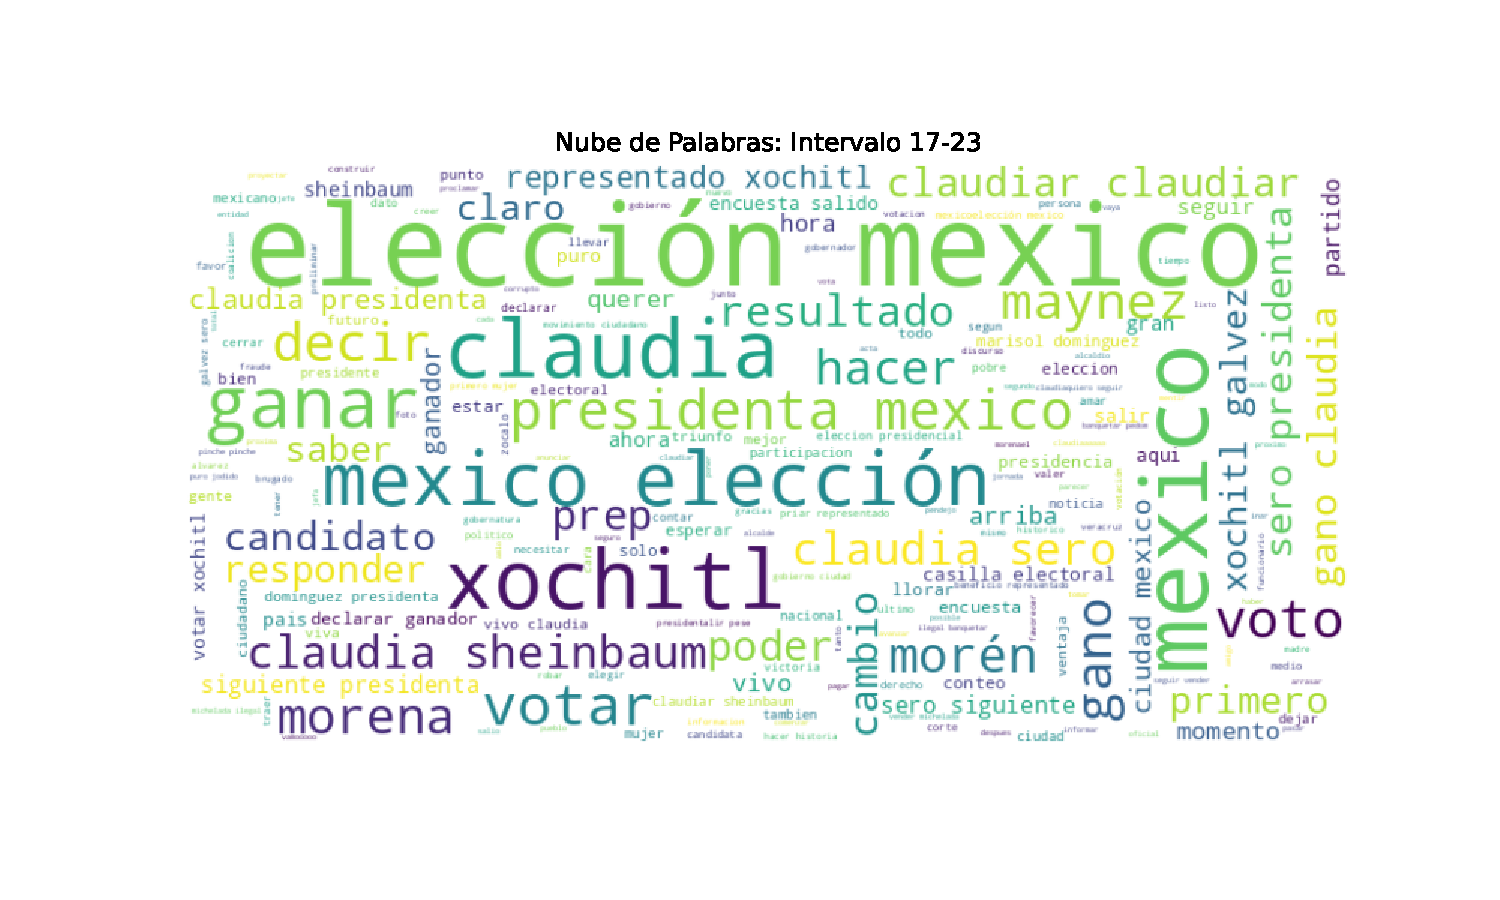
\includegraphics[width=\linewidth]{nube_intervalo_17-23.pdf}
			\vspace{-10mm}
			\caption{Nube de Palabras en el Horario de 08:00 a 12:00}
			\label{fig:nubeIntervalo1723}
		\end{minipage}
	\end{figure}

	En la nube general del día de la elección destaca términos como \textit{elección mexico}, \textit{votar}, \textit{siguiente presidenta}, \textit{xochitl galvez}. Esto refleja el enfoque de los usuarios en la jornada electoral, con énfasis en los principales candidatos y la participación ciudadana, indicando el interés por el proceso democrático.
	
	Y por intervalos, describimos a continuación las observaciones por cada uno:
	
	\begin{itemize}
		\item \textbf{Intervalo 8-12:} Las menciones predominantes incluyen términos como \textit{voto}, \textit{arrasar votación} y etiquetas relacionadas con ambos candidatos principales. Este periodo se caracteriza por mensajes incentivando el voto temprano y la participación.
		
		\item \textbf{Intervalo 12-17:} Se mantiene el protagonismo de \textit{votar xóchitl} y \textit{siguiente presidenta}, junto con menciones a \textit{casilla electoral}. Refleja el progreso del día y el aumento de interacciones relacionadas con el acto de votar.
		
		\item \textbf{Intervalo 17-23:} En las últimas horas, destacan términos como \textbf{ganar}, \textit{prep} y \textit{Claudia}. Esto indica una transición hacia la expectativa de resultados y comentarios finales sobre el cierre de casillas.
	\end{itemize}
	En general, las nubes reflejan cómo la narrativa cambia a lo largo del día, desde promover la participación hasta debatir resultados y candidatos clave.
	
	
	\subsubsection{Análisis de Engagement (YouTube)}
	
	En esta sección se analiza el nivel de interacción que generan los comentarios en los debates presidenciales, utilizando como indicador el número de \textit{me gusta} (num\_likes) para comprender las opiniones y temas que generaron mayor resonancia entre los usuarios.
	
	\begin{table}[H]
		\centering
		\begin{tabular}{|c|p{11cm}|c|c|}
			\hline
			\textbf{ID} & \textbf{Comentario} & \textbf{Num Likes} & \textbf{Num Debate} \\ \hline
			3831 & Es en serio lo que dijo la candidata Xochitl. ¿Pregúntenle a los muertos?. Que tonterías dice y sin razón. & 823 & 1 \\ \hline
			3848 & Imagínense que Xochitl quedara de presidente. No mms la peor vergüenza mundial que nos podría pasar & 745 & 1 \\ \hline
			3832 & Xochitl galvez es un peña nieto cualquiera & 717 & 1 \\ \hline
			3839 & Xóchitl se pone nerviosa en un debate y se traba al expresarse. Imagínate para dirigir un país & 661 & 1 \\ \hline
			2529 & Bla bla bla. A estas alturas. Ya sabemos quién miente. No somos pendejos. & 545 & 3 \\ \hline
		\end{tabular}
		\caption{Comentarios con mayor numero de likes en los debates presidenciales}
		\label{tab:comentarios_xochitl}
	\end{table}

	
	Observaciones sobre los comentarios más populares
	
	Los comentarios con mayor número de \textit{me gusta} tienden a centrarse en juicios hacia los candidatos, utilizando un tono crítico y humorístico. En particular, los cinco comentarios más populares observados tienen en común:
	
	\begin{itemize}
		\item \textbf{Foco en Xóchitl Gálvez:} Todos los comentarios hacen referencia directa a Xóchitl, lo que sugiere que su participación en los debates generó un alto nivel de interacción.
		\item \textbf{Tono crítico o sarcástico:} Los usuarios tienden a usar ironías o críticas contundentes, que parecen captar más atención y \textit{me gusta}.
		\item \textbf{Debate predominante:} Cuatro de los cinco comentarios están relacionados con el primer debate, lo que indica que este evento pudo haber generado el mayor nivel de controversia y participación.
	\end{itemize}
	
	
	\subsubsection{Análisis de Longitud y Complejidad de Comentarios}
	En esta sección se evalúa la longitud de los comentarios en YouTube y las publicaciones en la plataforma X, medida en cantidad de palabras. Este análisis permite comprender la complejidad y nivel de detalle de las interacciones en ambas plataformas. Se utiliza la longitud promedio como un indicador clave y se visualiza mediante histogramas que muestran la distribución de la frecuencia de palabras. Además, una línea punteada roja señala el promedio, ayudando a identificar si los comentarios suelen ser más extensos o concisos. Este enfoque facilita detectar patrones relacionados con la profundidad de las opiniones de los usuarios.
	
	\begin{figure}[h!]
		\centering
		\begin{minipage}{0.49\textwidth} % Mitad del ancho de la página
			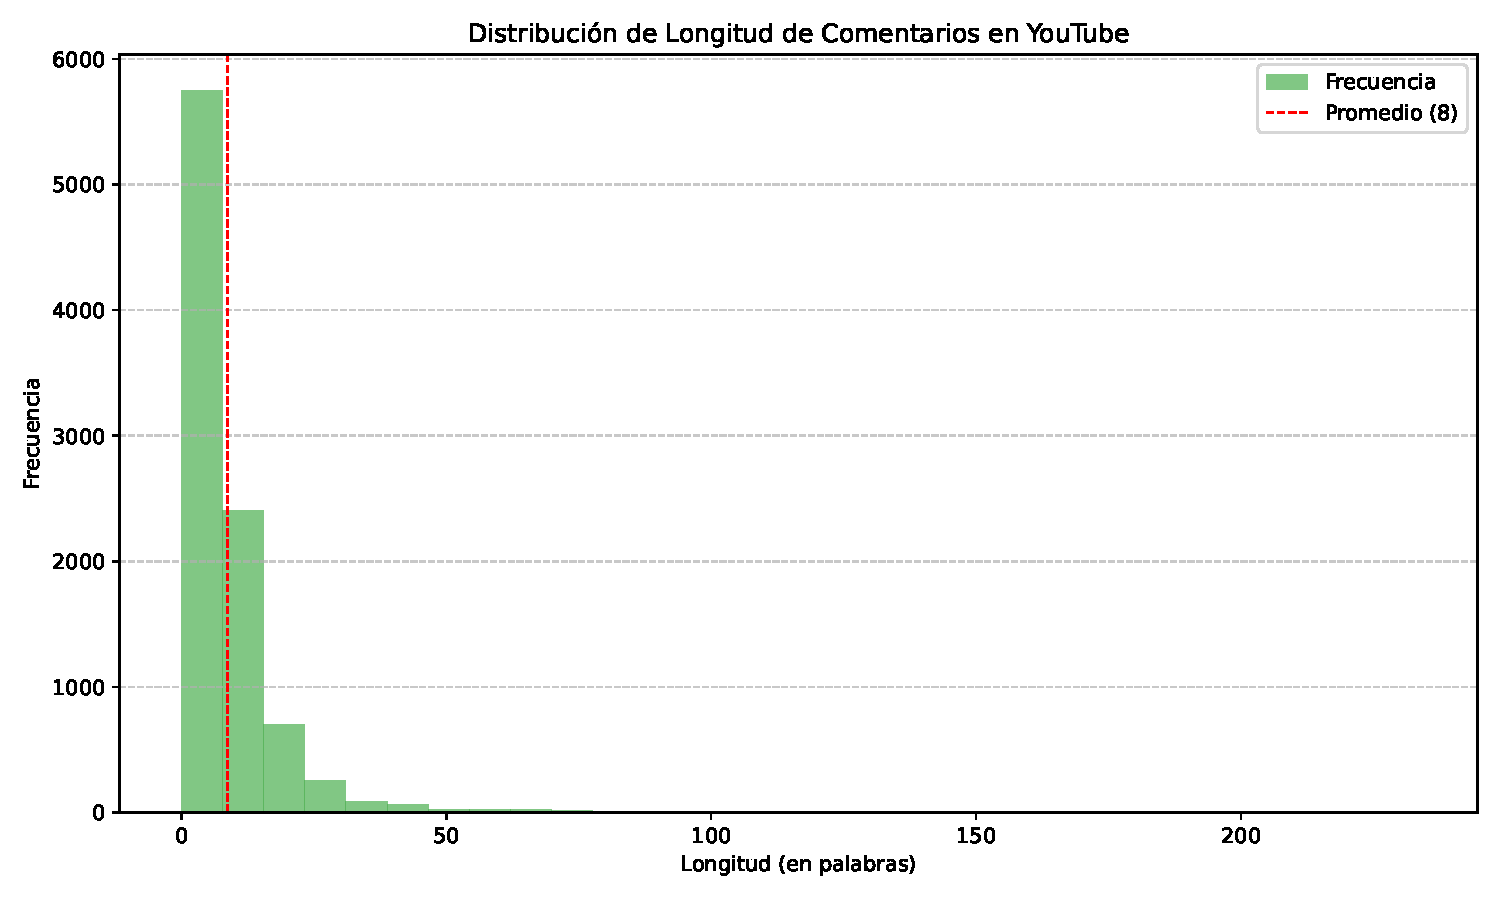
\includegraphics[width=\linewidth]{longitud_comentarios_youtube.pdf} 
			\vspace{-2mm}
			\caption{Distribución de Longitud de Comentarios en Youtube}
			\label{fig:longYoutube}
		\end{minipage}
		\hfill % Espacio flexible entre las dos imágenes
		\begin{minipage}{0.49\textwidth}
			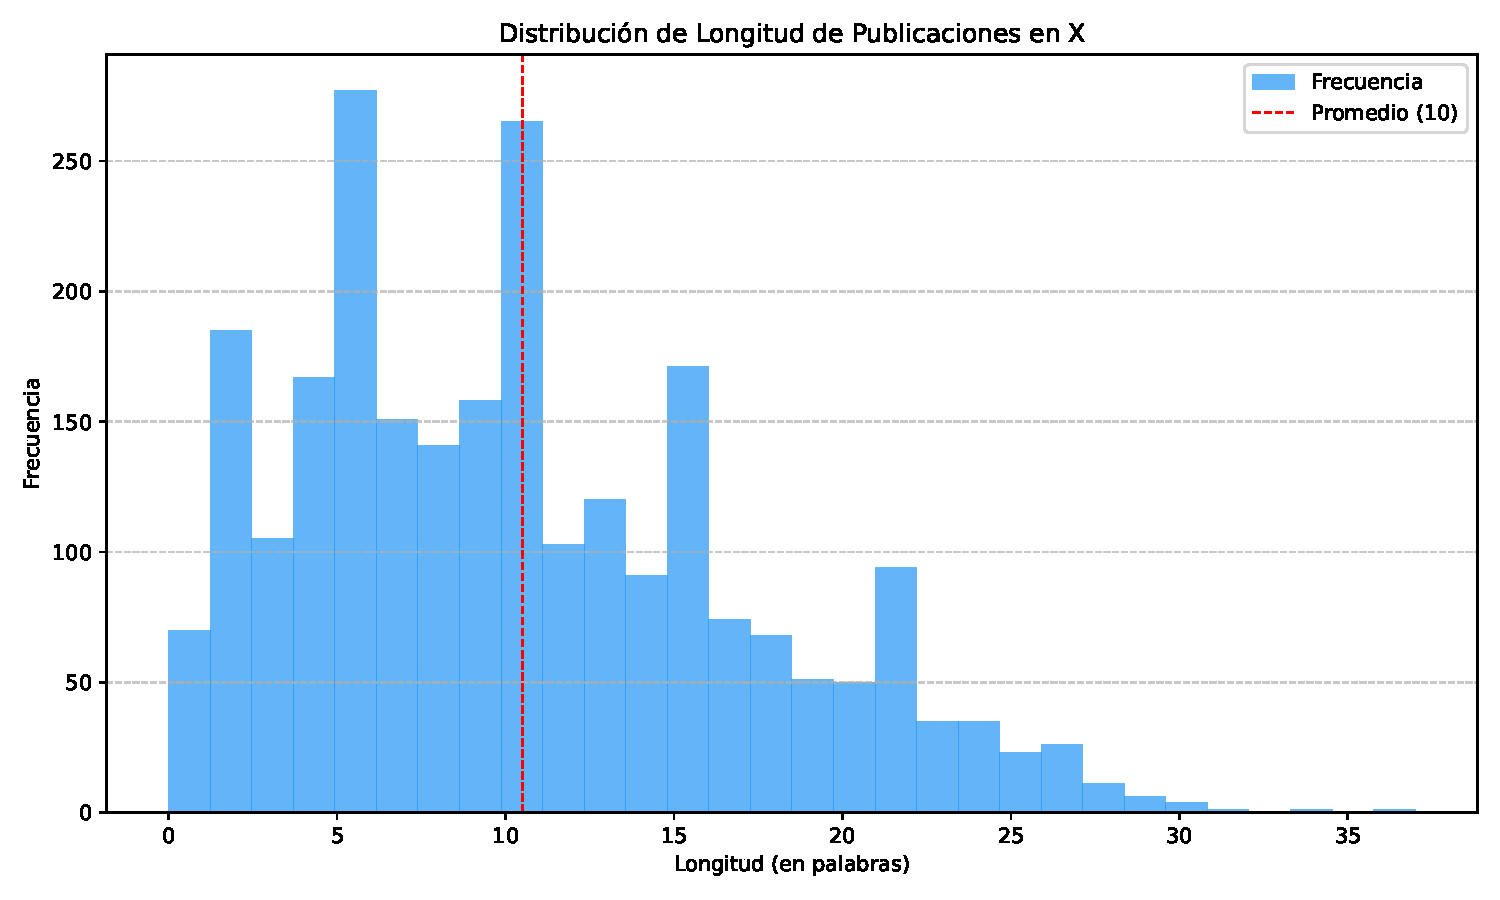
\includegraphics[width=\linewidth]{longitud_publicaciones_x.pdf}
			\vspace{-2mm}
			\caption{Distribución de Longitud de Publicaciones en X}
			\label{fig:longX}
		\end{minipage}
	\end{figure}
	
	
	En los histogramas presentados se observa la distribución de la longitud de los comentarios y publicaciones en los datasets de YouTube (figura \ref{fig:longYoutube}) y X (figura \ref{fig:longX}), respectivamente.
	
	\begin{enumerate}
		\item \textbf{YouTube:} La mayoría de los comentarios tienen una longitud muy corta, con un promedio de 8 palabras. Esto indica que los usuarios en esta plataforma tienden a realizar aportaciones concisas, posiblemente debido a la naturaleza del contenido de YouTube, que fomenta interacciones rápidas y directas. Sin embargo, hay una pequeña cantidad de comentarios que alcanzan longitudes mayores, reflejando una profundidad ocasional en el discurso.
		
		\item \textbf{X:} Las publicaciones en X también muestran un comportamiento de longitud predominantemente corto, con un promedio ligeramente menor, de 10 palabras. Esto puede atribuirse al formato de la plataforma, históricamente restringido en caracteres, lo que impulsa a los usuarios a ser breves. Sin embargo, se observa una mayor variabilidad en las longitudes en comparación con YouTube, con publicaciones que alcanzan hasta más de 30 palabras, posiblemente reflejando usuarios aprovechando la extensión actualizada de caracteres.
	\end{enumerate}
	
	\subsubsection{Conclusiones Preliminares}
	\textbf{De la Participación por Fecha y Plataforma:} En YouTube, la mayor cantidad de comentarios se concentra en el primer debate, disminuyendo ligeramente en los debates posteriores. Esto sugiere que el interés disminuyó conforme avanzaron los debates. En X, las publicaciones se distribuyen de manera más uniforme a lo largo del día de la elección, con un pico notable en los intervalos de la tarde, entre las 12:00 y 17:00, indicando una mayor actividad cuando se reportan resultados preliminares o momentos clave.
	
	\textbf{De las Menciones a Candidatos:} En ambos datasets, Claudia Sheinbaum y Xóchitl Gálvez presentan una proporción similar de menciones, reflejando su protagonismo en la conversación electoral. Jorge Álvarez Maynez tiene una participación significativamente menor.Un alto porcentaje de comentarios no menciona explícitamente a ningún candidato, lo que puede implicar discusiones generales sobre los debates o temas relacionados con la elección sin una referencia directa a los candidatos.
	
	\textbf{De la Frecuencia de Palabras:} En las nubes de palabras de los debates, los términos más frecuentes están relacionados con \textit{decir}, \textit{hacer}, \textit{propuestas} y los nombres de los candidatos, reflejando un enfoque en las declaraciones y promesas durante los debates. En el día de la elección, destacan palabras como \textit{elecciones mexico}, \textit{votar}, \textit{casilla} y \textit{resultados}, lo que subraya la interacción centrada en el acto de votar y la espera de resultados.
	
	\textbf{Del Engagement (YouTube):} Los comentarios con mayor número de likes tienden a ser más críticos o emocionales, especialmente hacia ciertos candidatos, lo que sugiere que las opiniones polarizadas generan mayor interacción.
	
	\textbf{De la Longitud y Complejidad:} Los comentarios en YouTube tienen un promedio de 8 palabras, mientras que las publicaciones en X tienen un promedio de 7 palabras, reflejando la naturaleza breve y directa de las interacciones en ambas plataformas. En ambas plataformas, la distribución de longitud es altamente sesgada hacia comentarios muy cortos, con pocas interacciones más elaboradas.
	
	\textbf{\textit{Resumen General}}
	
	Los resultados reflejan patrones importantes de participación y discurso en redes sociales durante el contexto electoral. Los candidatos principales, Claudia Sheinbaum y Xóchitl Gálvez, dominan la conversación, mientras que Jorge Álvarez Maynez tiene un impacto menor. Las palabras clave destacan el enfoque de los usuarios en propuestas y resultados, mientras que las interacciones tienden a ser breves y rápidas, acorde al formato de las plataformas.
	
	\subsection{Análisis de Sentimientos}
	Para analizar las opiniones expresadas en los comentarios y publicaciones de las redes sociales, se desarrolló un proceso de etiquetado de datos diseñado específicamente para capturar los matices del sentimiento en un contexto electoral multietiqueta. Este proceso consideró que un comentario puede expresar sentimientos hacia más de un candidato y, por tanto, el conjunto de datos se configuró para admitir múltiples etiquetas asociadas a un solo registro.
	
	\subsubsection{Codificación de Sentimientos}
	
	Se adoptó una codificación consistente para representar los sentimientos asociados a los candidatos principales de las elecciones presidenciales de México 2024, incluyendo un cuarto candidato virtual denominado \textit{Ninguno}. Este último se empleó en los casos donde los comentarios o publicaciones no hacían referencia explícita a ninguno de los candidatos reales. Las etiquetas se asignaron de la siguiente manera:
	
	\begin{itemize}
		\item \textbf{-1:} Sentimiento negativo hacia un candidato.
		\item \textbf{0:} Sentimiento neutral o ausencia de mención hacia el candidato en cuestión.
		\item \textbf{1:} Sentimiento positivo hacia un candidato.
	\end{itemize}
	
	Se establecieron lineamientos específicos para garantizar que las etiquetas reflejaran de manera precisa los sentimientos y opiniones expresados en los comentarios. Las principales consideraciones fueron las siguientes:
	
	\begin{enumerate}
		\item \textbf{Críticas al gobierno actual:} Se etiquetaron como sentimientos negativos hacia Claudia Sheinbaum, dado su vínculo con el partido en el poder.
		\item \textbf{Descalificaciones generales:} Comentarios como ``no hay ni a quién irle'' se etiquetaron con sentimiento negativo hacia los tres candidatos.
		\item \textbf{Críticas específicas a propuestas o lemas:} Cuando un comentario hacía referencia a una propuesta o lema de campaña, se marcó el sentimiento hacia el candidato que lo propuso.
		\item \textbf{Críticas a partidos o coaliciones:} En este caso, el sentimiento se asoció al candidato representante del partido o coalición mencionada.
		\item \textbf{Uso de apodos:} Se tuvo en cuenta el uso consistente de apodos en los comentarios para asociar el sentimiento con el candidato correspondiente.
	\end{enumerate}
	
	
	Se desarrolló una herramienta para facilitar este proceso, permitiendo asignar etiquetas a los comentarios de forma manual y precisa. La herramienta fue diseñada para soportar múltiples etiquetas por comentario, siguiendo la estructura multietiqueta del conjunto de datos. A continuación, se incluye una imagen que ilustra la interfaz y funcionalidad de esta herramienta:
	
	\begin{figure}[H]
		\centering
		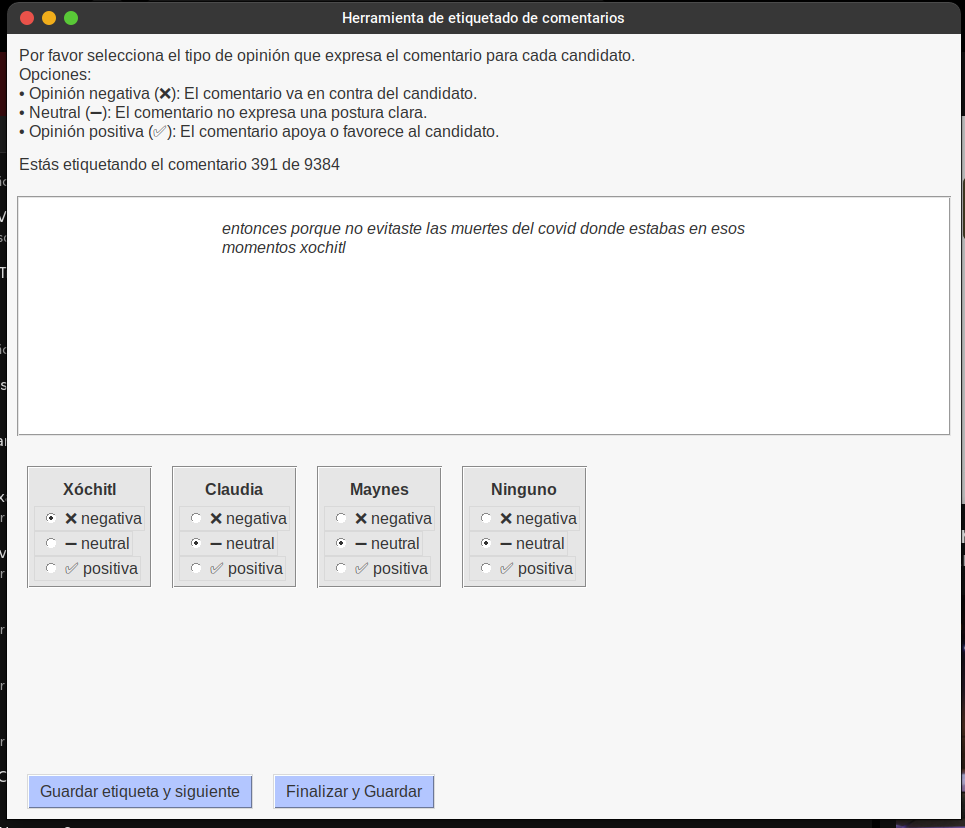
\includegraphics[width=0.6\textwidth]{etiquetado.png}
		\caption{Interfaz de la herramienta de etiquetado desarrollada para el análisis de sentimiento.}
		\label{fig:etiquetado}
	\end{figure}
	
	
	Como resultado del proceso de etiquetado descrito, se obtuvieron dos conjuntos de datos en formato tabular, el primero consta de 4,000 datos etiquetados correspondientes a los debates presidenciales, y el segundo con 1,000 datos etiquetados tomados de manera aleatoria del dia de la elección. Dichos datasets contienen las siguientes columnas adicionales:
	
	\begin{itemize}
		\item \texttt{Claudia:} Sentimiento expresado hacia Claudia Sheinbaum.
		\item \texttt{Maynez:} Sentimiento expresado hacia Jorge Álvarez Maynez.
		\item \texttt{Ninguno:} Sentimiento expresado hacia ningún candidato real.
		\item \texttt{Xóchitl:} Sentimiento expresado hacia Xóchitl Gálvez.
	\end{itemize}
	
	
	
	\subsubsection{BETO Fine-Tuning}
	
	Para la clasificación de sentimientos en los comentarios recopilados sobre los debates y el día de la elección, se realizó un proceso de fine-tuning del modelo pre-entrenado BETO (\textit{BERT en español}). Este modelo se adaptó para comprender el contexto político y la jerga mexicana relacionada con la jornada electoral de México 2024, permitiendo etiquetar automáticamente el resto de los comentarios no procesados manualmente.
	
	En primer lugar, para que el modelo de inteligencia pudiera entender mejor las etiquetas, se realizó una recodificación de los sentimientos:
	\begin{itemize}
		\item \(-1 \rightarrow 0\) (sentimiento negativo),
		\item \(0 \rightarrow 1\) (sentimiento neutral),
		\item \(1 \rightarrow 2\) (sentimiento positivo).
	\end{itemize}

	
	Se combinaron los dos conjuntos de datos (comentarios de debates y comentarios del día de la elección) en un único dataset con las siguientes columnas:
	\begin{itemize}
		\item \texttt{comentario\_editado}: Texto del comentario.
		\item \texttt{Claudia}, \texttt{Xóchitl}, \texttt{Maynez}, \texttt{Ninguno}: Etiquetas de sentimiento asociadas a cada candidato.
	\end{itemize}
	
	El problema se definió como una clasificación multietiqueta de tres clases (positivo, neutral y negativo) asociadas a cuatro categorías (los candidatos y la categoría ``Ninguno''). Esto resulta en un total de 12 clases (\(3 \times 4\)).
	
	Para combatir el desequilibrio en las clases, se realizaron los siguientes pasos:
	\begin{itemize}
		\item \textbf{Undersampling}: Se eliminaron 250 registros con etiquetas que indicaban sentimientos neutrales para los tres candidatos principales (\texttt{Xóchitl = 1, Claudia = 1, Maynez = 1}), buscando reducir el ruido en los datos.
		\item \textbf{Pesos de Clase}: Se utilizó la técnica \texttt{compute\_class\_weight} para calcular los pesos de clase, que luego fueron incorporados en una variante de la función de pérdida \texttt{CrossEntropyLoss}.
	\end{itemize}
	
	Propiamente hablando, el modelo fine-tuned incluyó los siguientes elementos:
	\begin{itemize}
		\item \textbf{BETO Pre-entrenado}: Se usó el token \texttt{[CLS]} como el vector de características representativo del significado global del comentario.
		\item \textbf{Clasificador Tipo MLP}: Se diseñó un perceptrón multicapa (MLP) cuya salida consistió en 12 logits:
		\begin{itemize}
			\item Logits \(0-2\): Sentimientos hacia Xóchitl.
			\item Logits \(3-5\): Sentimientos hacia Claudia.
			\item Logits \(6-8\): Sentimientos hacia Maynez.
			\item Logits \(9-11\): Sentimientos hacia Ninguno.
		\end{itemize}
		Para cada grupo de 3 logits se aplicó una función \texttt{softmax}, garantizando que las probabilidades en cada grupo sumen 1.
	\end{itemize}
	
	Dicho modelo se entrenó utilizando los siguientes parámetros: \(16\) en el tamaño del batch y \(3\) épocas de fine-tuning. 
	
	Con ello, el modelo fine-tuned logró un accuracy general del \textbf{81.3\%}, destacándose especialmente en la clasificación de sentimientos hacia \textbf{Xóchitl} con un 83.8\% de precisión, seguida de \textbf{Claudia} con un 81.2\% y \textbf{Maynez} con un 78.9\%. Las matrices de confusión revelan que el modelo clasificó correctamente la mayoría de los ejemplos neutrales, aunque los sentimientos negativos tendieron a confundirse con neutrales en algunos casos.
	
	\begin{figure}[h!]
		\centering
		\begin{minipage}{0.4\textwidth} % Mitad del ancho de la página
			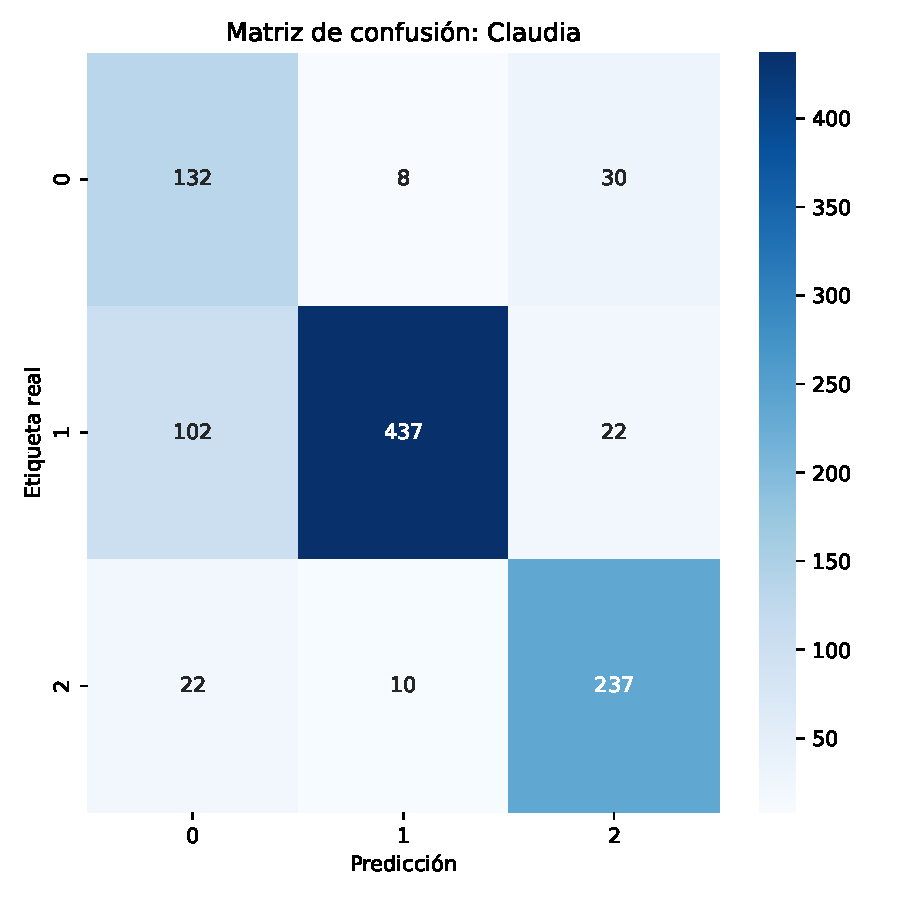
\includegraphics[width=\linewidth]{conf_matrix_Claudia.pdf} 
			\caption{Matriz de confusión para Claudia.}
			\label{fig:cmClaudia}
		\end{minipage}
		\hfill % Espacio flexible entre las dos imágenes
		\begin{minipage}{0.4\textwidth}
			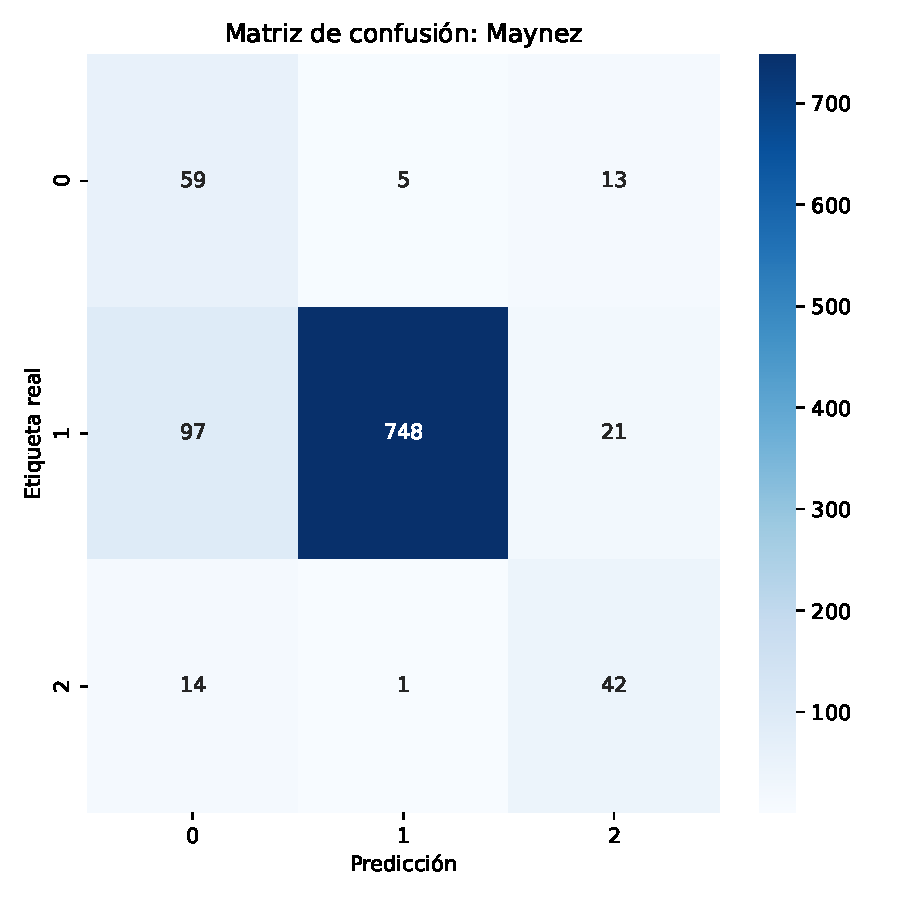
\includegraphics[width=\linewidth]{conf_matrix_Maynez.pdf}
			\caption{Matriz de confusión para Maynez.}
			\label{fig:cmMaynez}
		\end{minipage}
	\end{figure}
	
	\begin{figure}[h!]
		\centering
		\begin{minipage}{0.4\textwidth} % Mitad del ancho de la página
			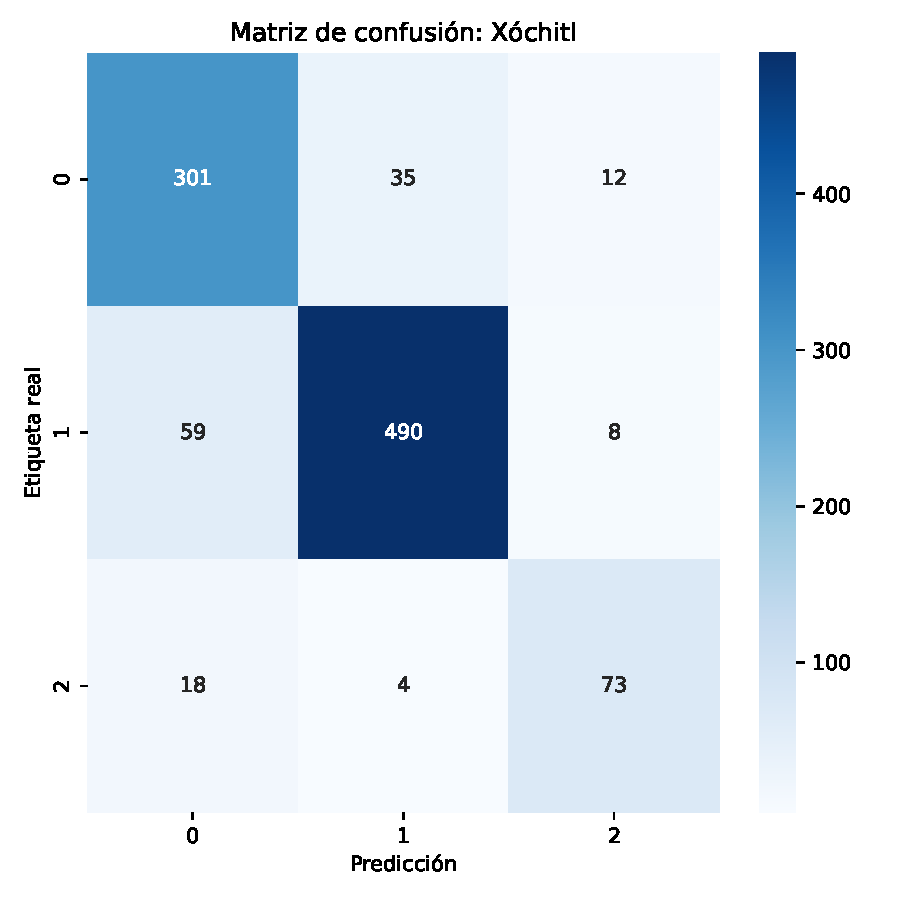
\includegraphics[width=\linewidth]{conf_matrix_Xóchitl.pdf} 
			\caption{Matriz de confusión para Xóchitl.}
			\label{fig:cmXochitl}
		\end{minipage}
	\end{figure}

	\vspace{-3mm}
	\begin{figure}[H]
		\centering
		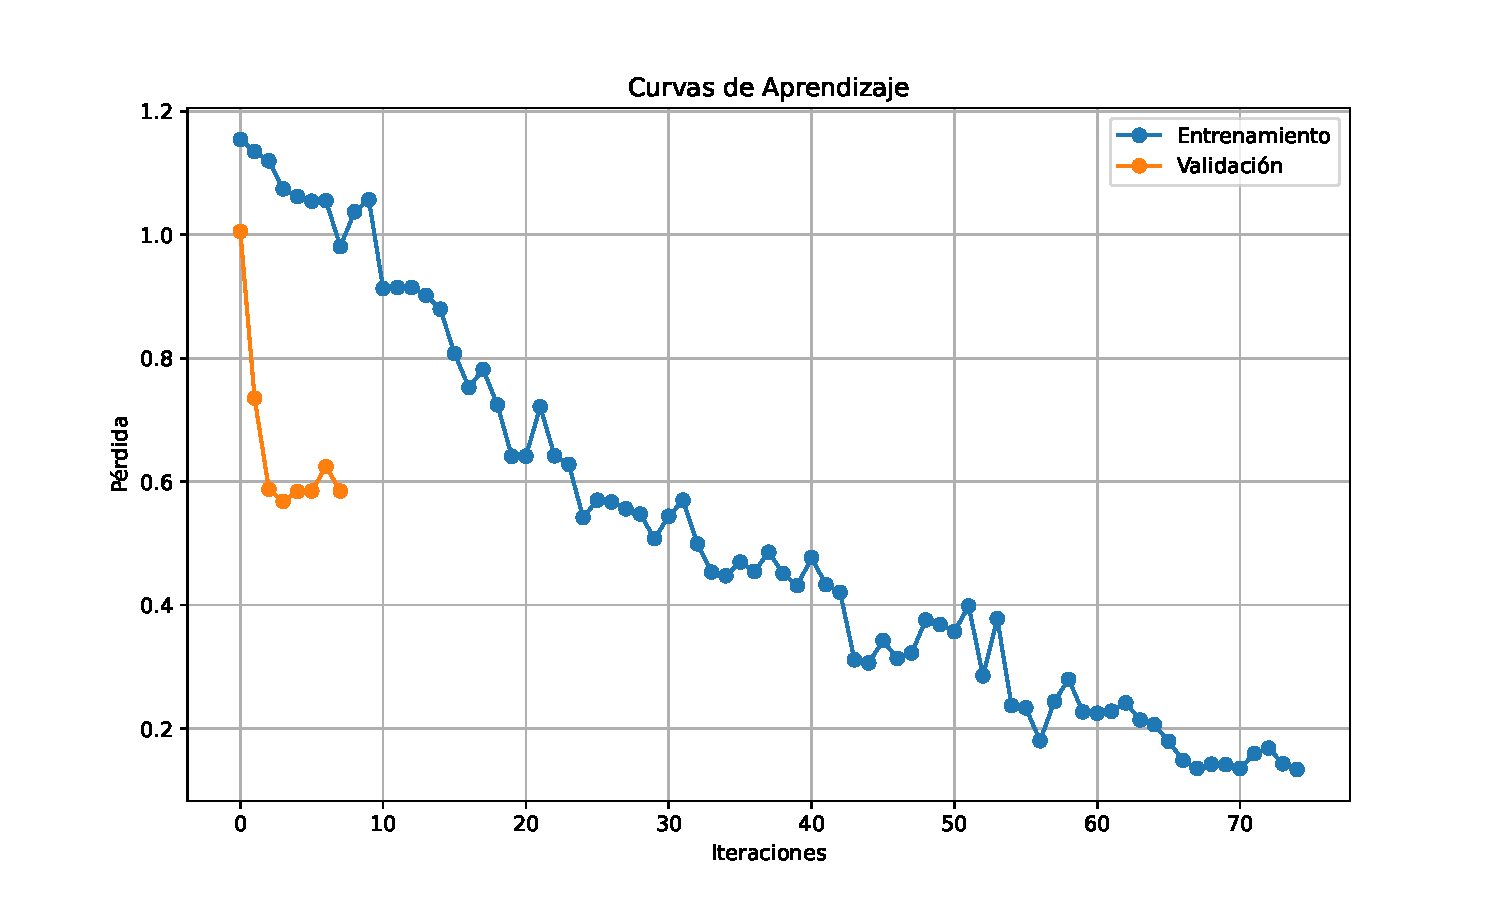
\includegraphics[width=0.65\textwidth]{curvas_de_perdida.pdf}
		\caption{Curva de pérdida durante el entrenamiento y validación.}
		\label{fig:curvaTrain}
	\end{figure}
	
	La gráfica de la función de pérdida de la figura \ref{fig:curvaTrain} muestra una disminución constante tanto en el entrenamiento como en la validación, lo que indica un aprendizaje efectivo y una convergencia adecuada hacia el final de las tres épocas. Además, la ausencia de divergencias entre las curvas sugiere que el modelo no presenta sobreajuste y generaliza bien al conjunto de validación.
	
	\subsubsection{Resultados del Análisis de Sentimientos}
	El análisis de sentimientos realizado en los comentarios recopilados de YouTube durante los debates presidenciales permitió identificar patrones de percepción pública hacia los candidatos principales: Claudia Sheinbaum, Xóchitl Gálvez y Jorge Álvarez Maynez. Los resultados, presentados en forma de gráficos que muestran la distribución porcentual de sentimientos (positivo, negativo y neutral) por cada candidato, reflejan diferencias importantes en la manera en que la audiencia reaccionó a los tres debates. A continuación, se describen las principales observaciones derivadas de este análisis.
	
	\textbf{Primer Debate Presidencial}
	\begin{itemize}
		\item \textbf{Claudia Sheinbaum} presentó una distribución equilibrada con un porcentaje significativo de comentarios neutrales (53.4\%) y un porcentaje considerable de positivos (23.8\%), lo que refleja una recepción mixta pero con un balance hacia lo positivo.
		\item \textbf{Jorge Álvarez Maynez} destacó por tener la mayor proporción de comentarios neutrales (75.6\%), indicando que su participación no generó tantas opiniones polarizadas. Sin embargo, los comentarios positivos fueron los más bajos (8.1\%) entre los tres candidatos.
		\item \textbf{Xóchitl Gálvez} enfrentó una proporción alta de comentarios negativos (42.0\%), siendo la candidata con mayor porcentaje de críticas negativas en este debate. Esto podría reflejar polarización en su percepción durante este evento.
	\end{itemize}
	\begin{figure}[H] % 'h!' posiciona la imagen cerca del texto relacionado
		\centering
		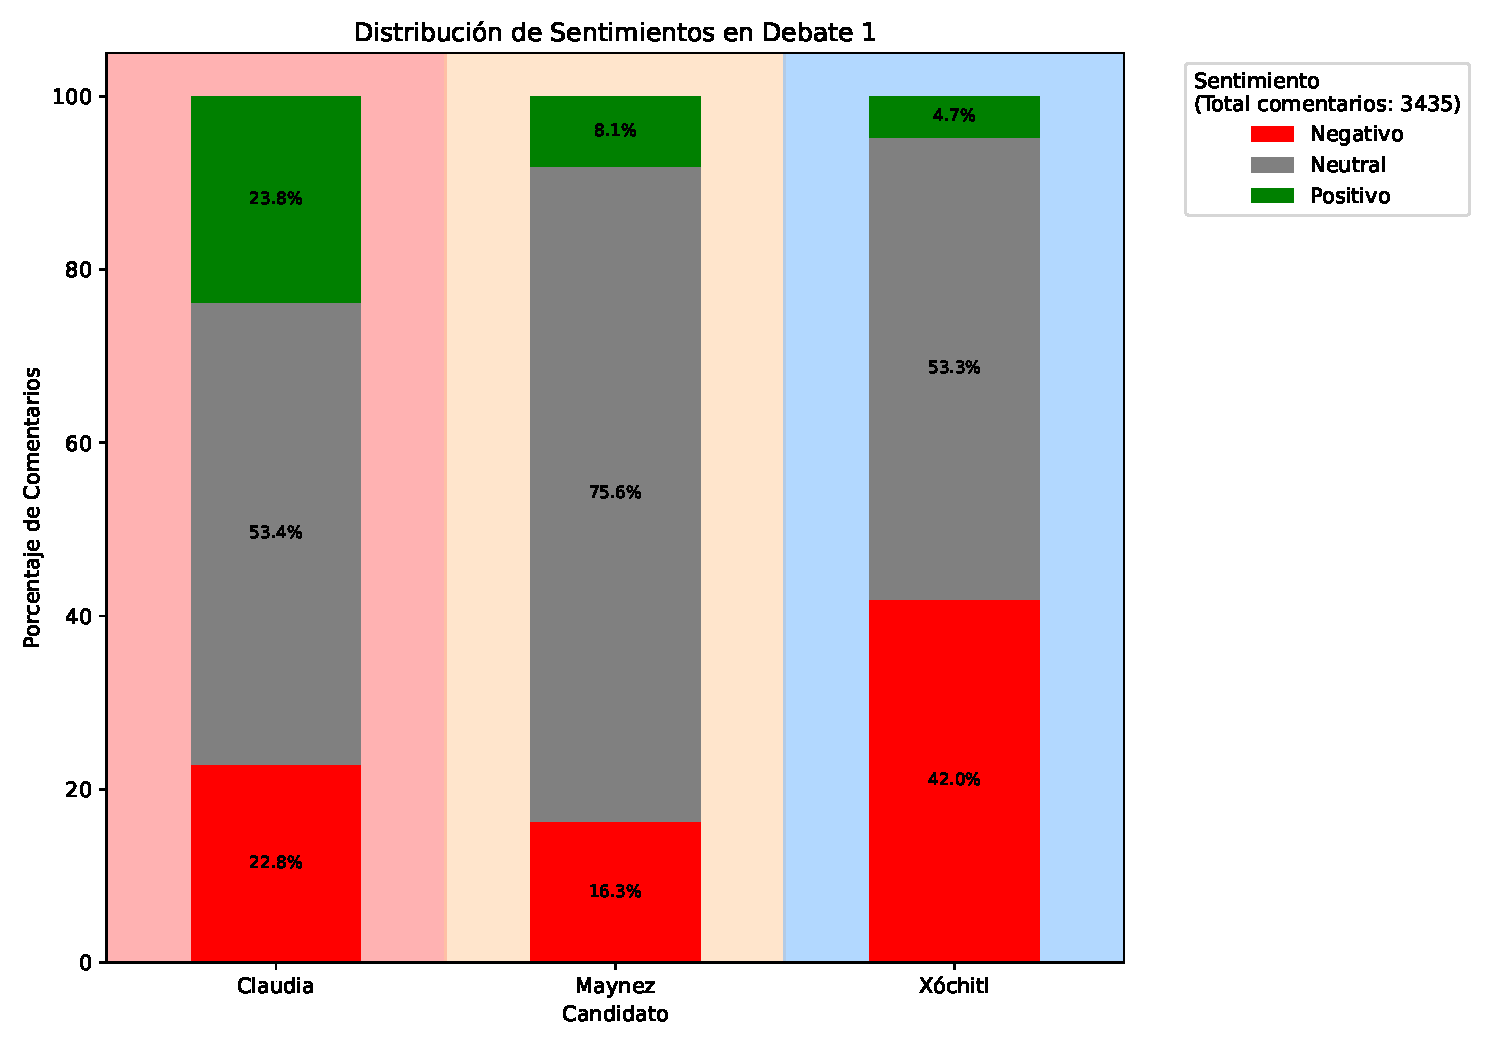
\includegraphics[width=0.8\textwidth]{sA_debate1.pdf} % Ajusta el tamaño con width o height
		\caption{Distribución de sentimientos en el primer debate} % Texto del caption
		\label{fig:sA_debate1} % Etiqueta para referenciar la imagen
	\end{figure}
	
	
	
	\textbf{Segundo Debate Presidencial}
	\begin{figure}[H] % 'h!' posiciona la imagen cerca del texto relacionado
		\centering
		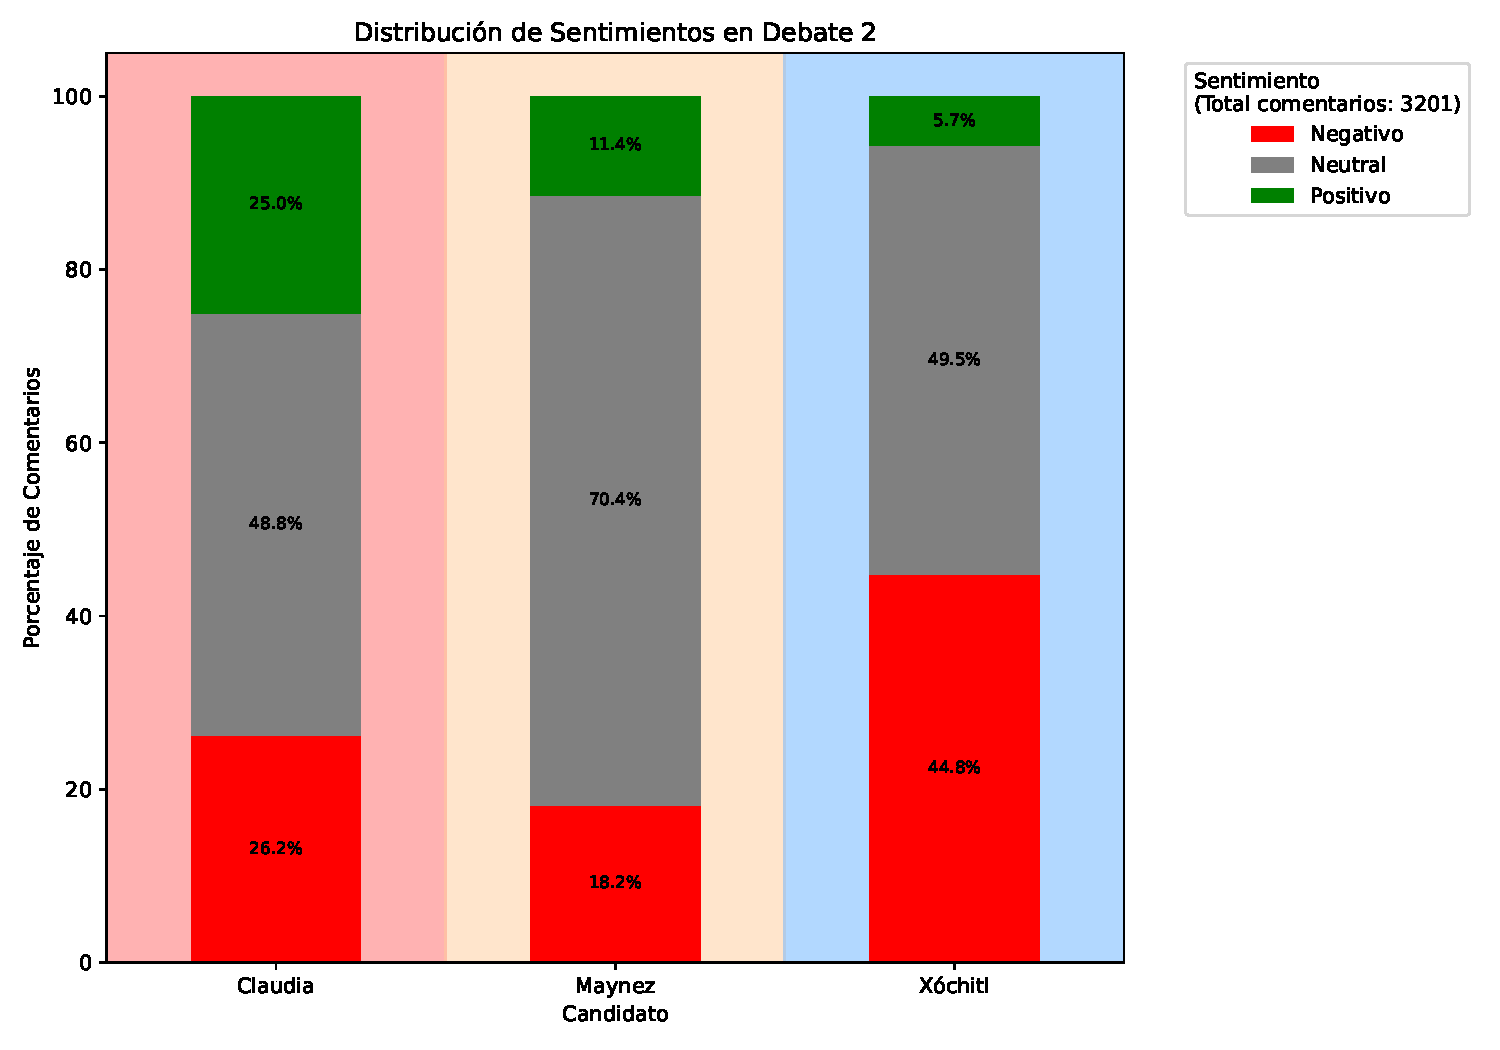
\includegraphics[width=0.75\textwidth]{sA_debate2.pdf} % Ajusta el tamaño con width o height
		\caption{Distribución de sentimientos en el segundo debate} % Texto del caption
		\label{fig:sA_debate2} % Etiqueta para referenciar la imagen
	\end{figure}
	\begin{itemize}
		\item \textbf{Claudia Sheinbaum} mejoró ligeramente en comentarios positivos (25.0\%) en comparación con el Debate 1, mientras que los neutrales se mantuvieron estables (48.8\%). Los negativos (26.2\%) indican un equilibrio en las opiniones.
		\item \textbf{Jorge Álvarez Maynez} continuó liderando en neutralidad (70.4\%) y mostró una mejora leve en la percepción positiva (11.4\%), sugiriendo una reacción más favorable en comparación con el primer debate.
		\item \textbf{Xóchitl Gálvez} experimentó una ligera reducción en comentarios negativos (44.8\%) pero aún mantiene un porcentaje elevado. Los comentarios positivos (5.7\%) siguen siendo los más bajos en comparación con los otros candidatos.
	\end{itemize}
	
	
	
	\textbf{Tercer Debate Presidencial}
	\begin{itemize}
		\item \textbf{Claudia Sheinbaum} alcanzó el porcentaje más alto de comentarios positivos (27.0\%) en el último debate, lo que puede interpretarse como una mejora en su percepción general. La neutralidad (52.3\%) se mantuvo constante y los comentarios negativos (20.6\%) disminuyeron.
		\item \textbf{Jorge Álvarez Maynez} continuó siendo el candidato con mayor neutralidad (77.3\%), mientras que los comentarios positivos (10.4\%) mostraron una ligera disminución, posiblemente indicando menor impacto en este debate.
		\item \textbf{Xóchitl Gálvez} no mostró cambios significativos en la percepción negativa (42.8\%), consolidando una imagen polarizada. La proporción de comentarios positivos (3.9\%) fue la más baja entre todos los debates y candidatos.
	\end{itemize}
	
	\begin{figure}[h!] % 'h!' posiciona la imagen cerca del texto relacionado
		\centering
		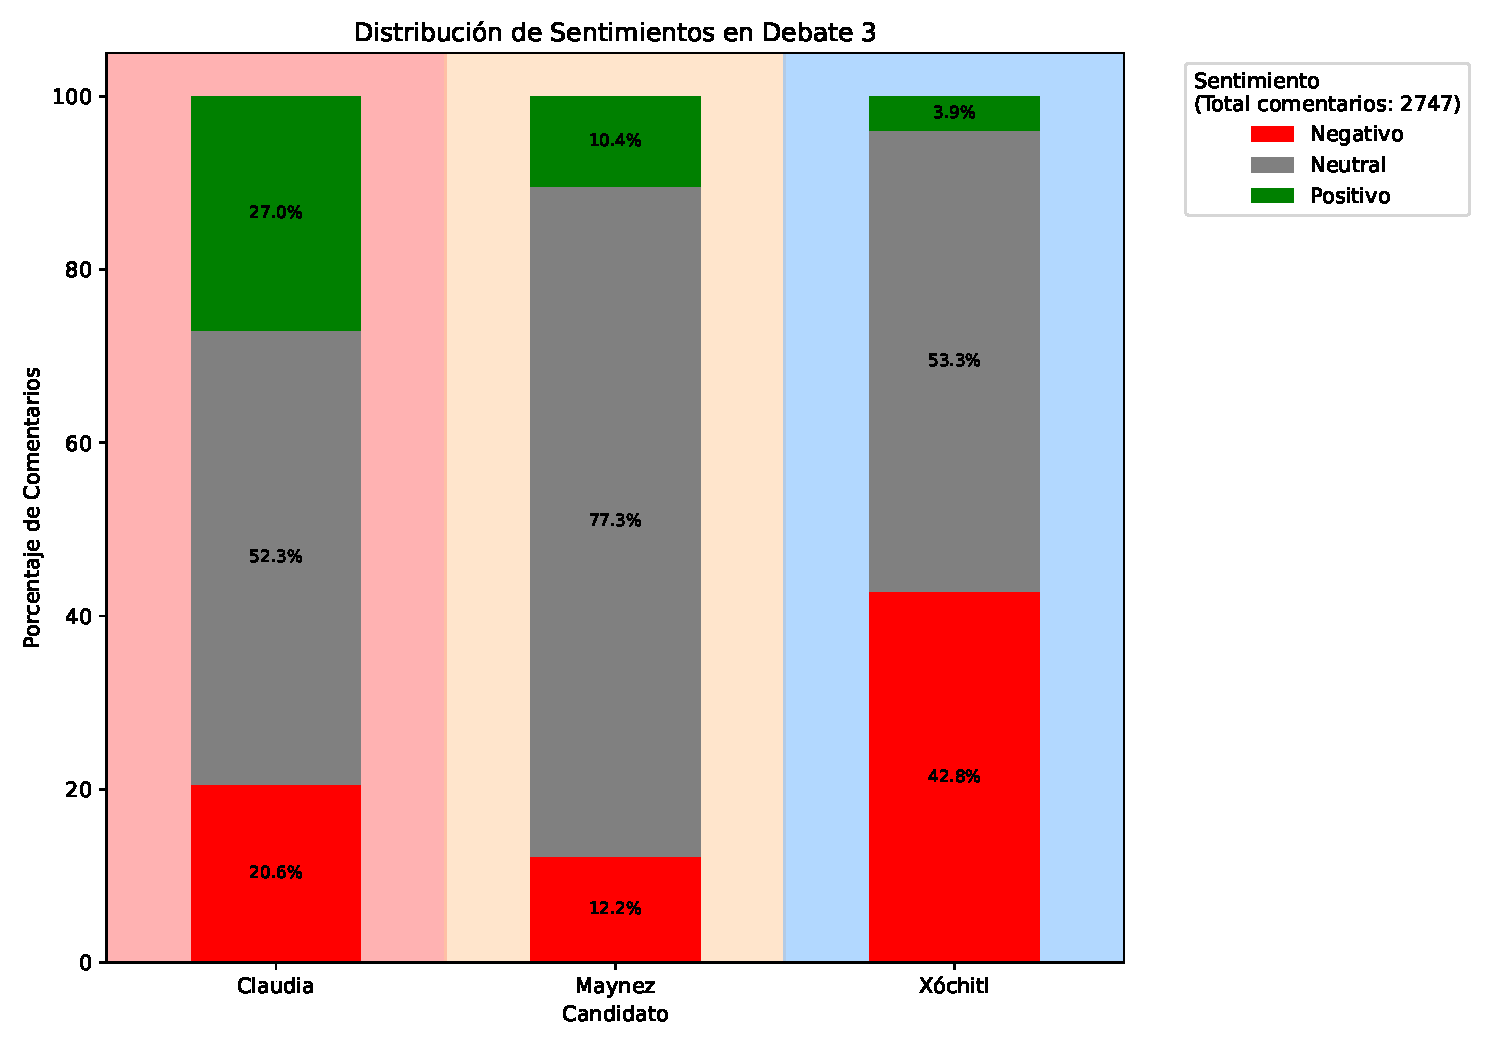
\includegraphics[width=0.75\textwidth]{sA_debate3.pdf} % Ajusta el tamaño con width o height
		\caption{Distribución de sentimientos en el tercer debate} % Texto del caption
		\label{fig:sA_debat3} % Etiqueta para referenciar la imagen
	\end{figure}
	
	En general, el análisis de sentimientos muestra que Claudia Sheinbaum mantuvo una percepción más equilibrada, con una tendencia hacia lo positivo a lo largo de los debates. Por otro lado, Xóchitl Gálvez enfrentó consistentemente una alta proporción de críticas negativas, mientras que Jorge Álvarez Maynez se posicionó como el candidato menos polarizante, con una abrumadora mayoría de comentarios neutrales. Estos resultados reflejan diferentes dinámicas en la percepción pública hacia los candidatos y su desempeño en los debates presidenciales.
	
	Los resultados del análisis de sentimientos en los debates presidenciales proporcionaron una visión general de cómo la percepción hacia los candidatos evolucionó a lo largo de los eventos clave del proceso electoral. 
	
	Sin embargo, el contexto de los debates presidenciales no es completamente representativo de la dinámica electoral en su conjunto. Es crucial explorar cómo las opiniones expresadas por el electorado evolucionaron durante el día de la elección, un evento crítico que concentra un alto volumen de interacción en redes sociales. Al analizar los comentarios realizados en intervalos de tiempo específicos a lo largo de este día, se identificaron patrones clave que reflejan el impacto inmediato del proceso de votación en la percepción pública.
	
	\vspace{3mm}
	\textbf{Dia de la Elección}
	
	
	\begin{figure}[h!] % 'h!' posiciona la imagen cerca del texto relacionado
		\centering
		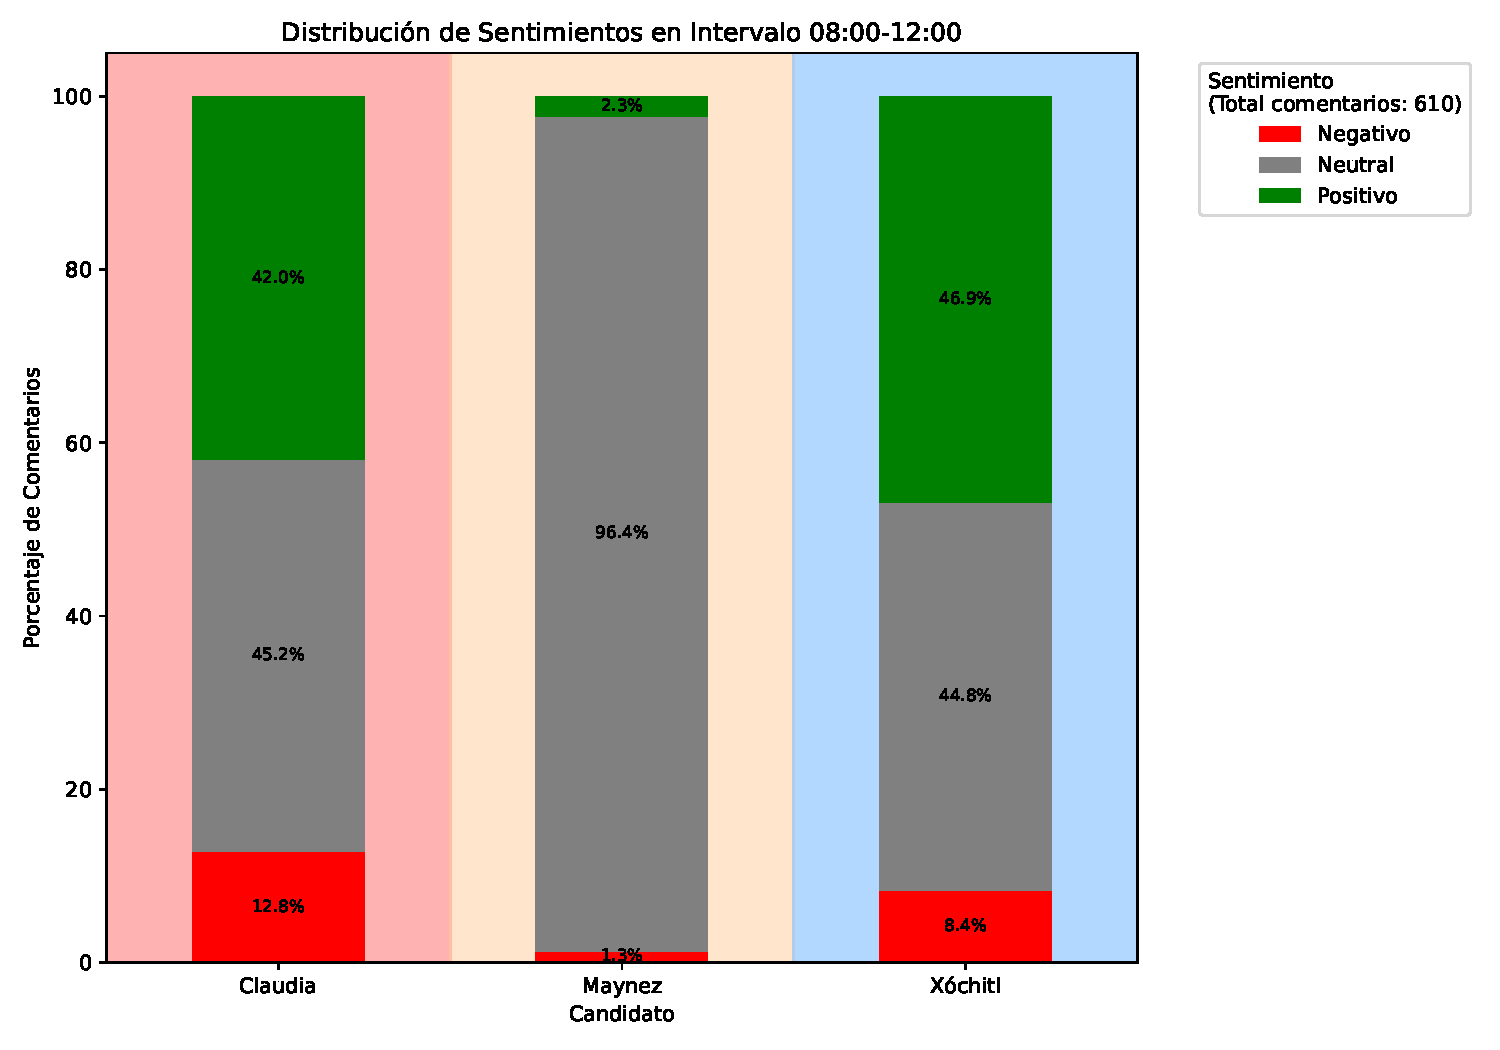
\includegraphics[width=0.73\textwidth]{sA_intervalo_0812.pdf} % Ajusta el tamaño con width o height
		\caption{Distribución de sentimientos en el horario 08:00 a 12:00} % Texto del caption
		\label{fig:sA_08a12} % Etiqueta para referenciar la imagen
	\end{figure}
	
	\begin{figure}[h!] % 'h!' posiciona la imagen cerca del texto relacionado
		\centering
		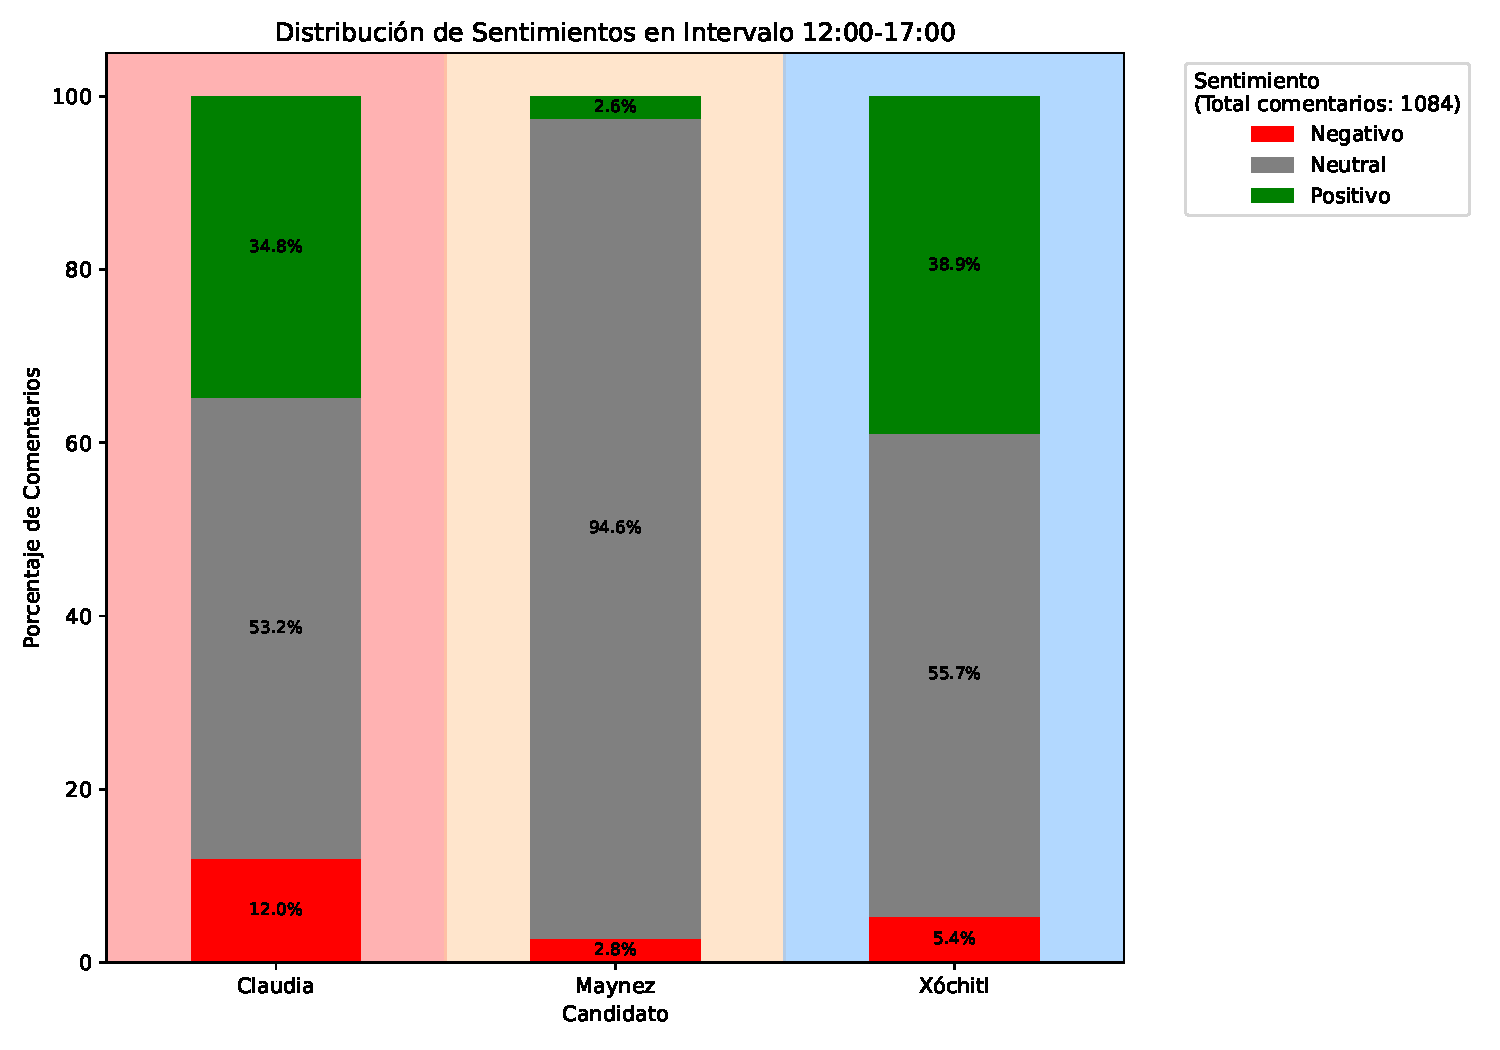
\includegraphics[width=0.73\textwidth]{sA_intervalo_1217.pdf} % Ajusta el tamaño con width o height
		\caption{Distribución de sentimientos en el horario 17:00 a 23:00} % Texto del caption
		\label{fig:sA_12a17} % Etiqueta para referenciar la imagen
	\end{figure}
	
	Los debates presidenciales habían planteado un escenario predecible pero diverso. Claudia Sheinbaum, con su discurso moderado, había conseguido un balance en las emociones del público; Xóchitl Gálvez, en cambio, dividía opiniones, y Jorge Álvarez Maynez parecía tener un perfil bajo, dejando a la audiencia más indiferente que comprometida. Pero el día de la elección prometía ser un escenario completamente distinto: un día donde la incertidumbre, la expectativa y las emociones se mezclan en tiempo real.
	
	A las 8:00 de la mañana, los primeros comentarios comenzaron a fluir en redes sociales. Entre el café y las urnas recién abiertas, los simpatizantes de Claudia y Xóchitl mostraban optimismo. Con un 42.0\% de comentarios positivos para Sheinbaum y un sorprendente 46.9\% para Gálvez, la mañana parecía brillar para estas candidatas. Mientras tanto, Jorge Álvarez Maynez seguía sin alterar demasiado las aguas: un 96.4\% de neutralidad marcaba una narrativa poco emocionante para él en las primeras horas del día.
	
	Al avanzar hacia el mediodía (12:00-17:00), las emociones comenzaron a estabilizarse. Sheinbaum, aunque aún sólida, bajó a un 34.8\% de comentarios positivos. Xóchitl, por su parte, conservó su lugar con un 38.9\%, mostrando que sus simpatizantes permanecían activos. Maynez, fiel a su tendencia, continuó siendo el candidato de las emociones contenidas, con un 94.6\% de neutralidad. Este tramo de la jornada parecía indicar que las audiencias se movían hacia un tono más reflexivo.
	
	\begin{figure}[H] % 'h!' posiciona la imagen cerca del texto relacionado
		\centering
		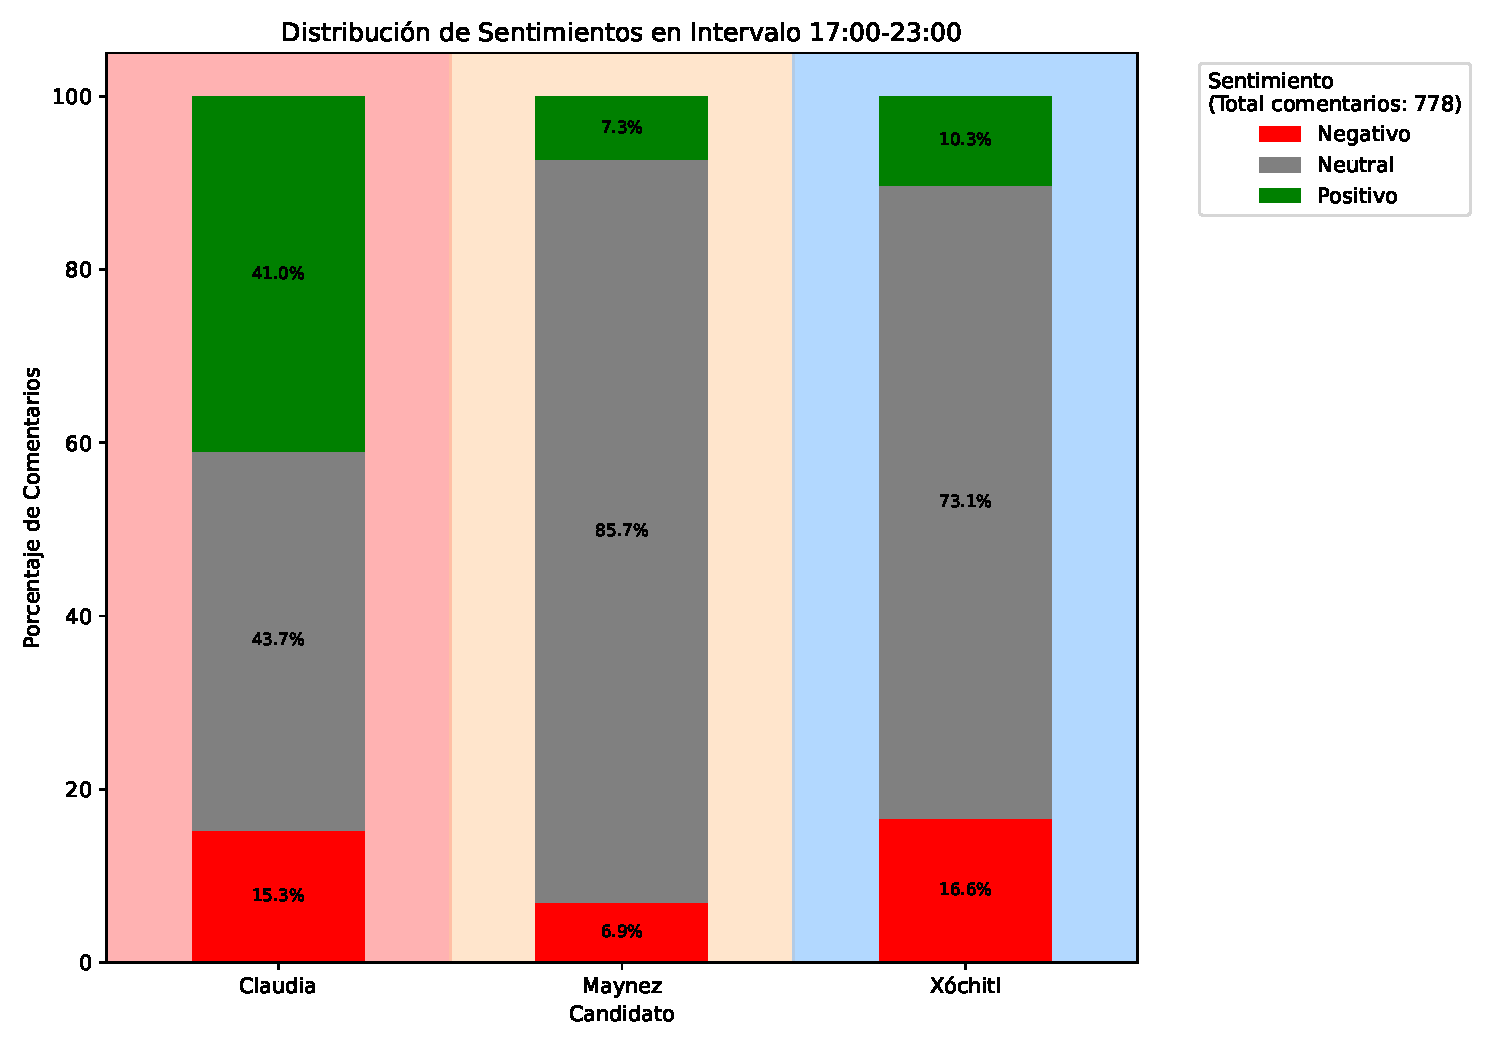
\includegraphics[width=0.73\textwidth]{sA_intervalo_1723.pdf} % Ajusta el tamaño con width o height
		\caption{Distribución de sentimientos en el horario 17:00 a 23:00} % Texto del caption
		\label{fig:sA_17a23} % Etiqueta para referenciar la imagen
	\end{figure}
	
	Sin embargo, conforme el sol se ocultaba, la narrativa cambiaba. De 17:00 a 23:00, Claudia Sheinbaum cerró el día con un repunte significativo: un 41.0\% de comentarios positivos y una notable disminución de negativos (15.3\%). Era como si el fin del proceso electoral hubiera favorecido su discurso. Para Xóchitl Gálvez, el cierre fue más desafiante. Aunque alcanzó un 10.3\% de comentarios positivos, los negativos subieron a un 16.6\%, consolidando su imagen polarizada. Maynez, sin grandes sorpresas, mantuvo su alto porcentaje de neutralidad (85.7\%), siendo nuevamente el menos discutido entre los candidatos.
	
	El día de la elección no solo reflejó las emociones de los votantes, sino también la intensidad de su conexión con los candidatos. Mientras Claudia Sheinbaum logró mantener una narrativa positiva y consistente, Xóchitl Gálvez navegó entre los extremos del apoyo y la crítica. Por otro lado, Jorge Álvarez Maynez quedó como el espectador silencioso de una conversación que nunca terminó de involucrarlo. Este análisis captura no solo los números, sino también la historia que contaron las audiencias en tiempo real, marcando un contraste fascinante con los debates presidenciales.
	
	
	\subsubsection{Comparación de Sentimientos entre los Debates y el Día de la Elección}
	
	El análisis de sentimientos a lo largo del proceso electoral permitió identificar cambios significativos en las emociones expresadas por los usuarios, marcando diferencias claras entre los debates presidenciales y el día de la elección.
	
	Durante los debates, las emociones estuvieron marcadas por una mayor polarización. Claudia Sheinbaum destacó con una proporción consistente de comentarios positivos, reflejando una percepción equilibrada que mejoró progresivamente a lo largo de los tres debates. Esta tendencia sugiere que su desempeño logró conectar con una parte significativa del electorado, generando confianza. Por otro lado, Xóchitl Gálvez enfrentó una alta proporción de comentarios negativos desde el primer debate, consolidando una percepción polarizada y crítica hacia su figura. A pesar de pequeñas variaciones, los comentarios negativos se mantuvieron constantes a lo largo de los debates, reflejando las dificultades que tuvo para mejorar su imagen entre los usuarios. Jorge Álvarez Maynez, en cambio, se posicionó como el candidato menos polarizante, con una abrumadora mayoría de comentarios neutrales. Este patrón indica que, si bien no generó controversia, tampoco logró captar suficiente atención o impacto entre la audiencia.
	
	El día de la elección marcó un cambio en el tono emocional de las conversaciones. Claudia Sheinbaum continuó dominando con comentarios mayoritariamente positivos, lo que refleja una consolidación de confianza y apoyo por parte de sus simpatizantes. Las emociones hacia Xóchitl Gálvez, aunque todavía polarizadas, mostraron un ligero aumento en la proporción de comentarios positivos durante las primeras horas del día, posiblemente impulsado por sus seguidores más activos. Sin embargo, los comentarios negativos hacia ella continuaron siendo significativos, reforzando la percepción crítica predominante. En cuanto a Jorge Álvarez Maynez, la neutralidad siguió siendo la emoción predominante, manteniéndose como un candidato que generó poca discusión o controversia en comparación con sus contrincantes.
	
	La principal diferencia entre los debates y el día de la elección radica en la intensidad y la dirección de las emociones. Durante los debates, el análisis reflejó un electorado crítico y atento, con emociones más divididas y opiniones formadas sobre los candidatos. En contraste, el día de la elección mostró un tono más emocional y optimista, con un enfoque en la experiencia de votar y en los resultados preliminares. Esto evidencia cómo el contexto y la naturaleza de cada evento influyen en las emociones expresadas por los usuarios en redes sociales, marcando una evolución en las percepciones a medida que avanzó el proceso electoral.
	
	
	
	\subsection{Modelado temático}
	
	El análisis de tópicos es una técnica del procesamiento de lenguaje natural que busca identificar temas subyacentes en grandes volúmenes de datos textuales. Este enfoque parte de la premisa de que los textos que comparten palabras o conceptos similares suelen estar relacionados semánticamente. Mediante técnicas de clusterización, es posible agrupar comentarios o publicaciones que tienen patrones lingüísticos comunes, lo que permite inferir temas principales a partir de cada grupo.
	
	La clusterización resulta eficaz porque organiza los datos textuales en conjuntos o \textit{clusters} que representan similitudes en su contenido. Cada cluster se interpreta como un conjunto de textos que gira en torno a un mismo tema, y al analizar las palabras más frecuentes o características de cada grupo, se pueden identificar las ideas centrales que lo definen. Por ejemplo, si un cluster contiene palabras como \textit{cambio}, \textit{progreso} y \textit{política}, es probable que el tema subyacente esté relacionado con propuestas de mejora o debates políticos.
	
	En este estudio, se utilizó el modelo BERTopic, una herramienta que combina tres componentes clave:
	\begin{itemize}
		\item \textbf{Embeddings semánticos:} Representan el significado de los textos en un espacio vectorial, donde textos similares están más cercanos.
		\item \textbf{Reducción de dimensionalidad:} Simplifica los datos para facilitar la visualización y el procesamiento sin perder relaciones importantes entre textos.
		\item \textbf{Clustering de alta densidad:} Agrupa los textos en clusters basados en la densidad de los puntos en el espacio reducido, lo que ayuda a identificar patrones semánticos consistentes.
	\end{itemize}
	
	El resultado es un conjunto de tópicos que representan los temas más discutidos dentro del corpus analizado. Este enfoque permite no solo identificar los temas principales, sino también cuantificar la cantidad de textos asociados a cada uno, proporcionando una visión clara de las dinámicas y preferencias expresadas en redes sociales.
	
	El proceso de análisis de tópicos se llevó a cabo en las siguientes etapas:
	
	
	\subsubsection{Preprocesamiento}
	Antes de generar los embeddings y proceder con el análisis de tópicos, se llevó a cabo un proceso de preprocesamiento de los comentarios recopilados de YouTube y X. Este paso es fundamental para garantizar que los datos textuales estén en un formato limpio y uniforme, facilitando así la extracción de características relevantes. El preprocesamiento incluyó las siguientes tareas:
	
	\begin{itemize}
		\item \textbf{Conversión a texto:} Todos los comentarios fueron convertidos a cadenas de texto para evitar problemas con valores nulos o datos de tipo incorrecto.
		\item \textbf{Eliminación de palabras vacías (\textit{stopwords}):} Se utilizó una función personalizada para remover palabras comunes del idioma español que no aportan significado semántico (como \textit{el, la, de}, etc.). Esto permitió enfocar el análisis en términos más relevantes para los datos.
		\item \textbf{Limpieza de texto:} Se eliminaron caracteres especiales, espacios en blanco excesivos y elementos irrelevantes para el análisis, dejando únicamente el contenido textual procesado.
	\end{itemize}
	
	
	\subsubsection{BETO Embeddings}
	Para capturar las características semánticas de los datos textuales, se utilizaron embeddings generados con el modelo BETO. Estos embeddings representan cada texto en un espacio vectorial de alta dimensionalidad, preservando relaciones semánticas entre las palabras y frases, dicho vector de características resultante de este modelo comparte las mismas propiedades que el detallado en la sección Análisis de Sentimientos.

	\subsubsection{Reducción de Dimensionalidad}
	Dado que trabajar con datos en alta dimensionalidad puede ser computacionalmente costoso, se aplicó la técnica UMAP (\textit{Uniform Manifold Approximation and Projection}) para reducir la dimensionalidad de los embeddings. Este método preserva tanto la estructura local como la global de los datos. Los hiperparámetros clave utilizados fueron:
	
	\begin{itemize}
		\item \textbf{n\_neighbors = 15:} Define el número de vecinos locales considerados para construir la estructura de los datos. Este valor logra un equilibrio entre capturar estructuras locales y globales.
		\item \textbf{n\_components = 2:} Reduce los datos a dos dimensiones, facilitando la visualización y el agrupamiento.
		\item \textbf{metric = 'cosine':} Utiliza la distancia coseno, una métrica adecuada para datos textuales, ya que mide la similitud angular entre vectores.
		\item \textbf{random\_state = 42:} Asegura la reproducibilidad de los resultados al fijar una semilla para la generación aleatoria.
	\end{itemize}

	
	\subsubsection{Clusterización}
	Despues, para identificar agrupamientos en el espacio reducido, se empleó el algoritmo HDBSCAN (\textit{Hierarchical Density-Based Spatial Clustering of Applications with Noise}). Este método es una extensión de DBSCAN y se caracteriza por:
	
	\begin{itemize}
		\item \textbf{Adaptabilidad a densidades variables:} A diferencia de DBSCAN, HDBSCAN detecta clusters en datos con densidades desiguales.
		\item \textbf{Tolerancia al ruido:} Etiqueta puntos con baja densidad como ruido, lo que mejora la calidad de los clusters.
	\end{itemize}
	
	Los hiperparámetros predeterminados utilizados fueron:
	\begin{itemize}
		\item \textbf{min\_cluster\_size = 5:} Número mínimo de documentos requeridos para formar un cluster.
		\item \textbf{min\_samples:} Calculado automáticamente como \(1.5 \times\) \textit{min\_cluster\_size}, controla la clasificación de puntos como ruido.
		\item \textbf{metric = 'euclidean':} Métrica de distancia utilizada por defecto.
		\item \textbf{cluster\_selection\_epsilon = 0.0:} Define la tolerancia para formar clusters, con un valor estricto predeterminado.
	\end{itemize}

	Se calculó el coeficiente de silueta para evaluar la cohesión interna y separación de los clusters formados. Este coeficiente varía entre -1 y 1, donde valores cercanos a 1 indican una buena formación del cluster. Los resultados se representaron mediante un gráfico de siluetas y una visualización en 2D de los clusters generados.
	
	Los temas identificados se almacenaron en un archivo \texttt{topics.csv} con las siguientes columnas:
	\begin{itemize}
		\item \textbf{evento:} Identifica el evento al que corresponde (debate 1, debate 2, debate 3 o día de la elección).
		\item \textbf{fecha:} Fecha del evento.
		\item \textbf{Topic:} Palabra clave principal asignada al cluster.
		\item \textbf{Count:} Número de comentarios asociados al cluster.
		\item \textbf{Name:} Identificador del cluster.
		\item \textbf{silhouette\_promedio:} Promedio del coeficiente de silueta del cluster.
	\end{itemize}
	
	Posteriormente, se generó un archivo filtrado \texttt{selected\_topics.csv}, que contiene únicamente los clusters con mayor número de comentarios (\texttt{Count}) y un coeficiente de silueta mayor a 0.5, considerado como un umbral que garantiza una buena cohesión y evidencia suficiente de formación del cluster.

	Los resultados del análisis de tópicos se presentan en dos formas:
	\begin{itemize}
		\item \textbf{Gráfico de Clusters en 2D:} Una representación visual de los clusters generados en el espacio reducido.
		\item \textbf{Gráfico de Siluetas:} Evalúa la cohesión y separación de cada cluster, permitiendo interpretar la calidad de los agrupamientos.
	\end{itemize}
	
	
	\subsubsection{Resultados del Modelado Temático}
	
	El análisis de los resultados obtenidos mediante BERTopic se centra en evaluar la calidad de los clusters generados y su relevancia para identificar los temas principales de los debates y el día de la elección presidencial. A través de las gráficas de silueta, se evalúa la cohesión interna y separación de cada cluster, lo que permite determinar su consistencia. Estas gráficas muestran cómo se distribuyen los coeficientes de silueta para los documentos dentro de cada cluster, donde valores más altos (cercanos a 1) indican mayor cohesión dentro del cluster y mejor separación respecto a otros clusters.
	
	A continuación, se presenta el análisis individual de las gráficas de silueta para cada evento, comenzando con la representación visual de cada gráfica.
	
	\vspace{4mm}
	\textbf{Debate 1}
	\begin{figure}[h!]
		\centering
		\begin{minipage}{0.49\textwidth} % Mitad del ancho de la página
			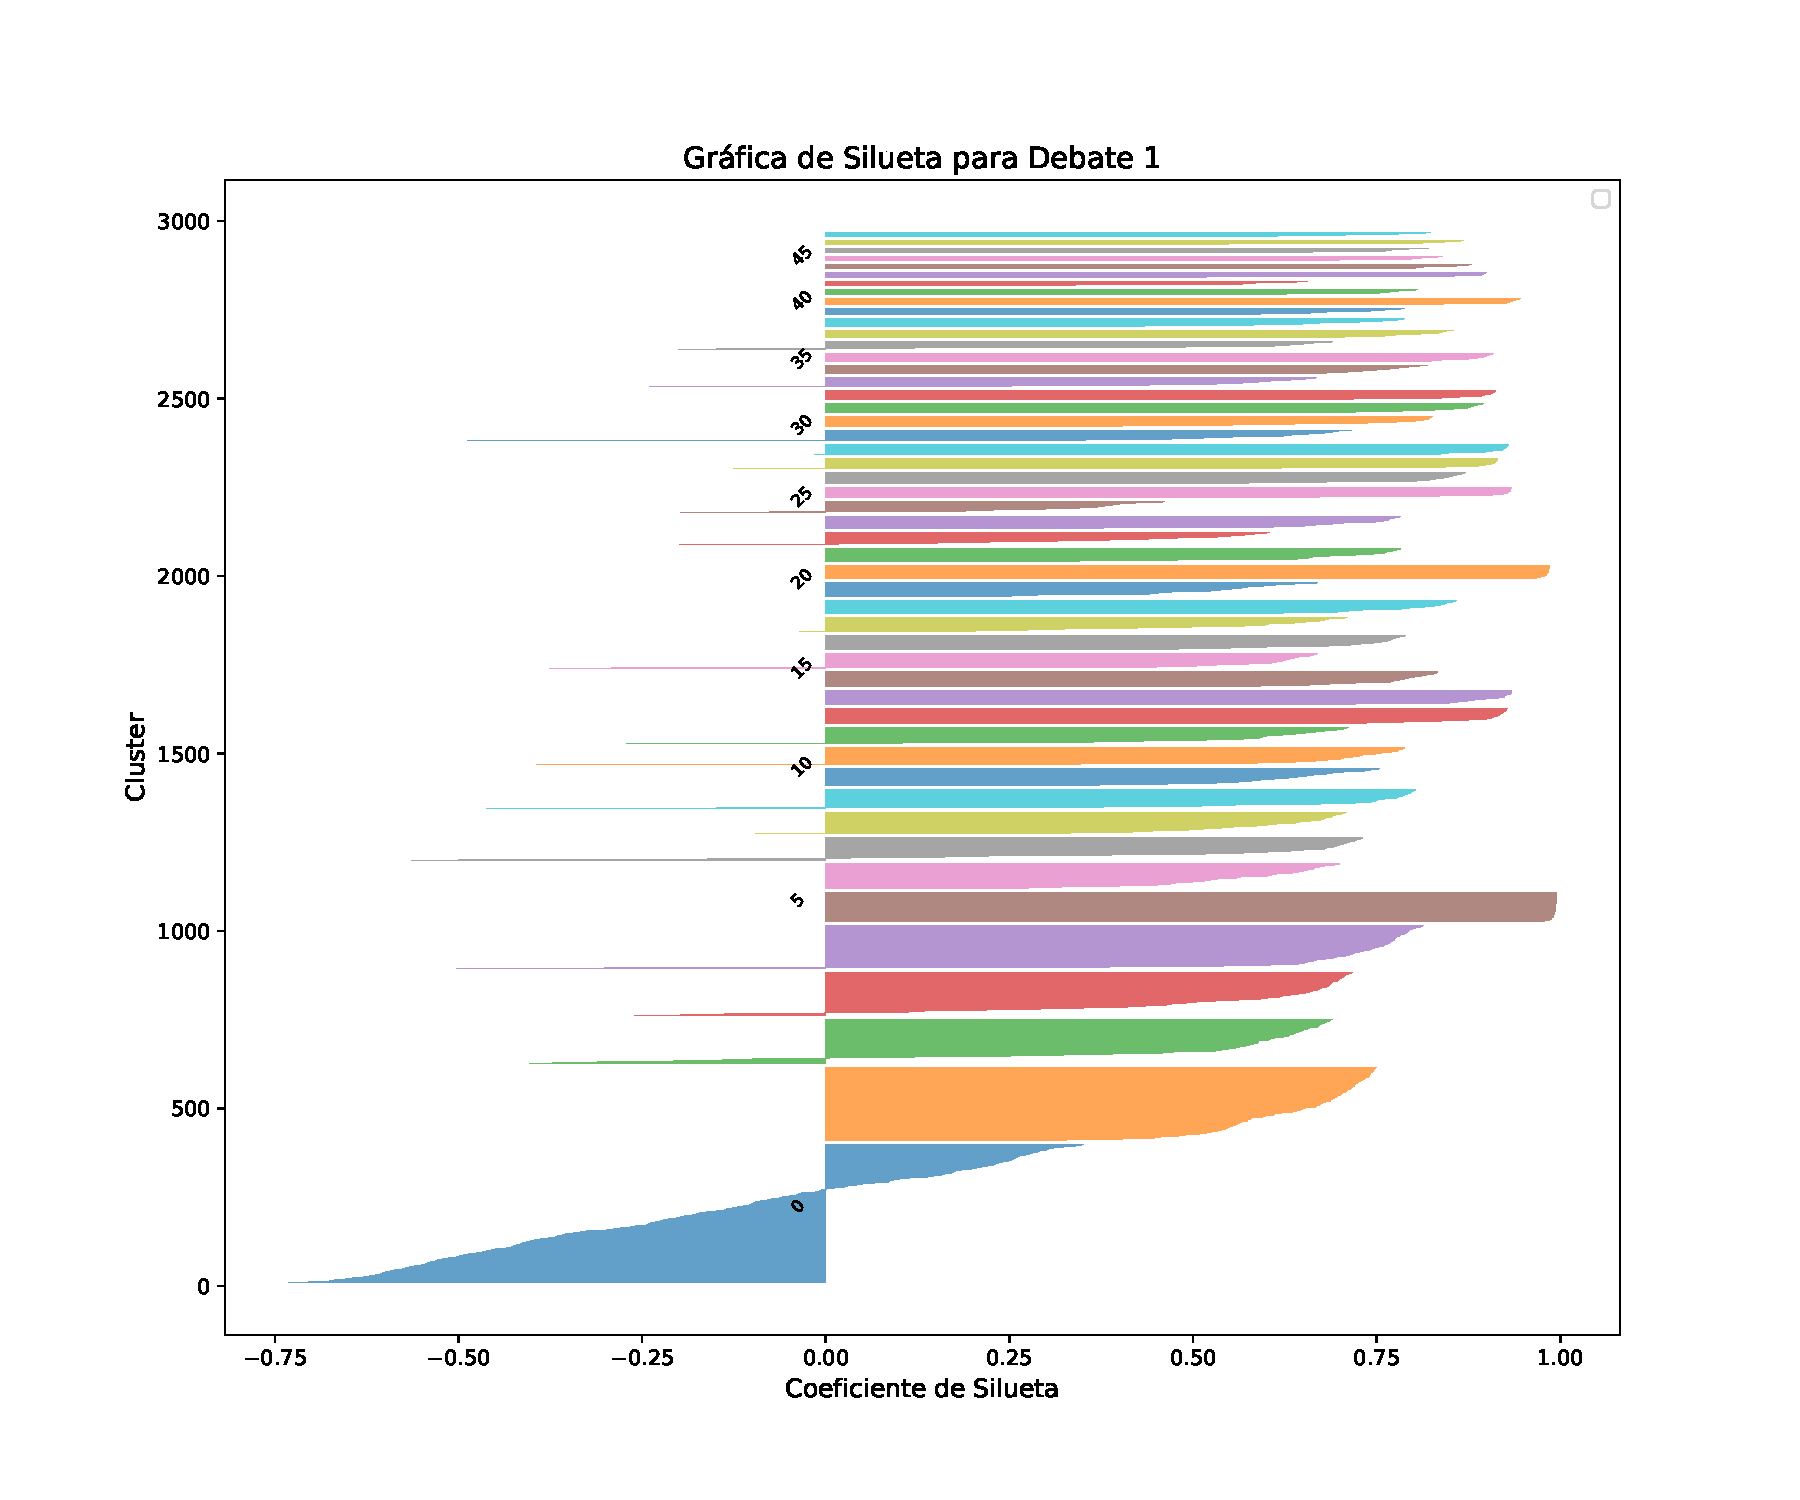
\includegraphics[width=\linewidth]{silhouette_debate1.pdf} 
			\caption{Gráfica de Silueta para el primer debate}
			\label{fig:silDeb1}
		\end{minipage}
		\hfill % Espacio flexible entre las dos imágenes
		\begin{minipage}{0.49\textwidth}
			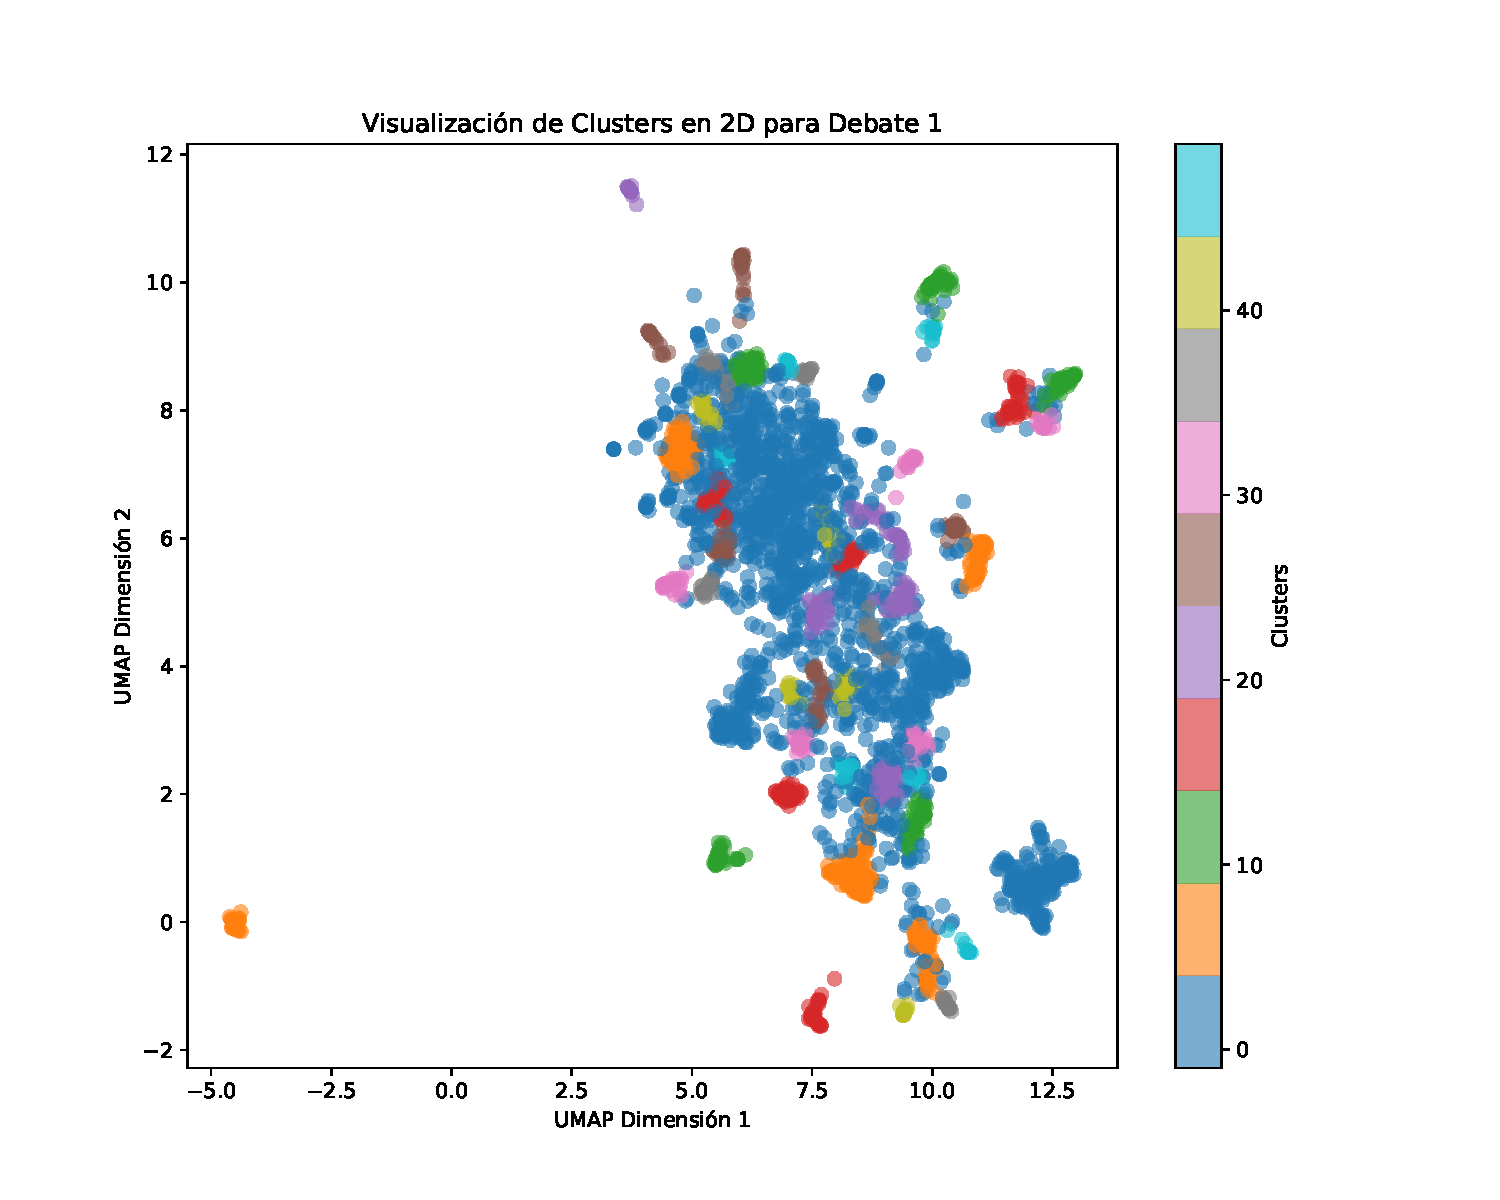
\includegraphics[width=\linewidth]{clusters_debate1.pdf}
			\caption{Grafica de clusters del primer debate}
			\label{fig:clustDeb1}
		\end{minipage}
	\end{figure}
	
	En la gráfica correspondiente a la figura \ref{fig:silDeb1}, se observa una gran cantidad de clusters con coeficientes de silueta positivos, lo que indica que la mayoría de los clusters tienen buena cohesión interna. Sin embargo, también hay varios clusters con valores de silueta cercanos a cero o negativos, lo que refleja una posible superposición de temas o documentos ambiguos. Los clusters más grandes tienden a tener mejores valores de cohesión, lo que podría deberse a que capturan temas centrales con una gran cantidad de comentarios relacionados.
	
	\vspace{4mm}
	\textbf{Debate 2}

	\begin{figure}[h!]
		\centering
		\begin{minipage}{0.49\textwidth} % Mitad del ancho de la página
			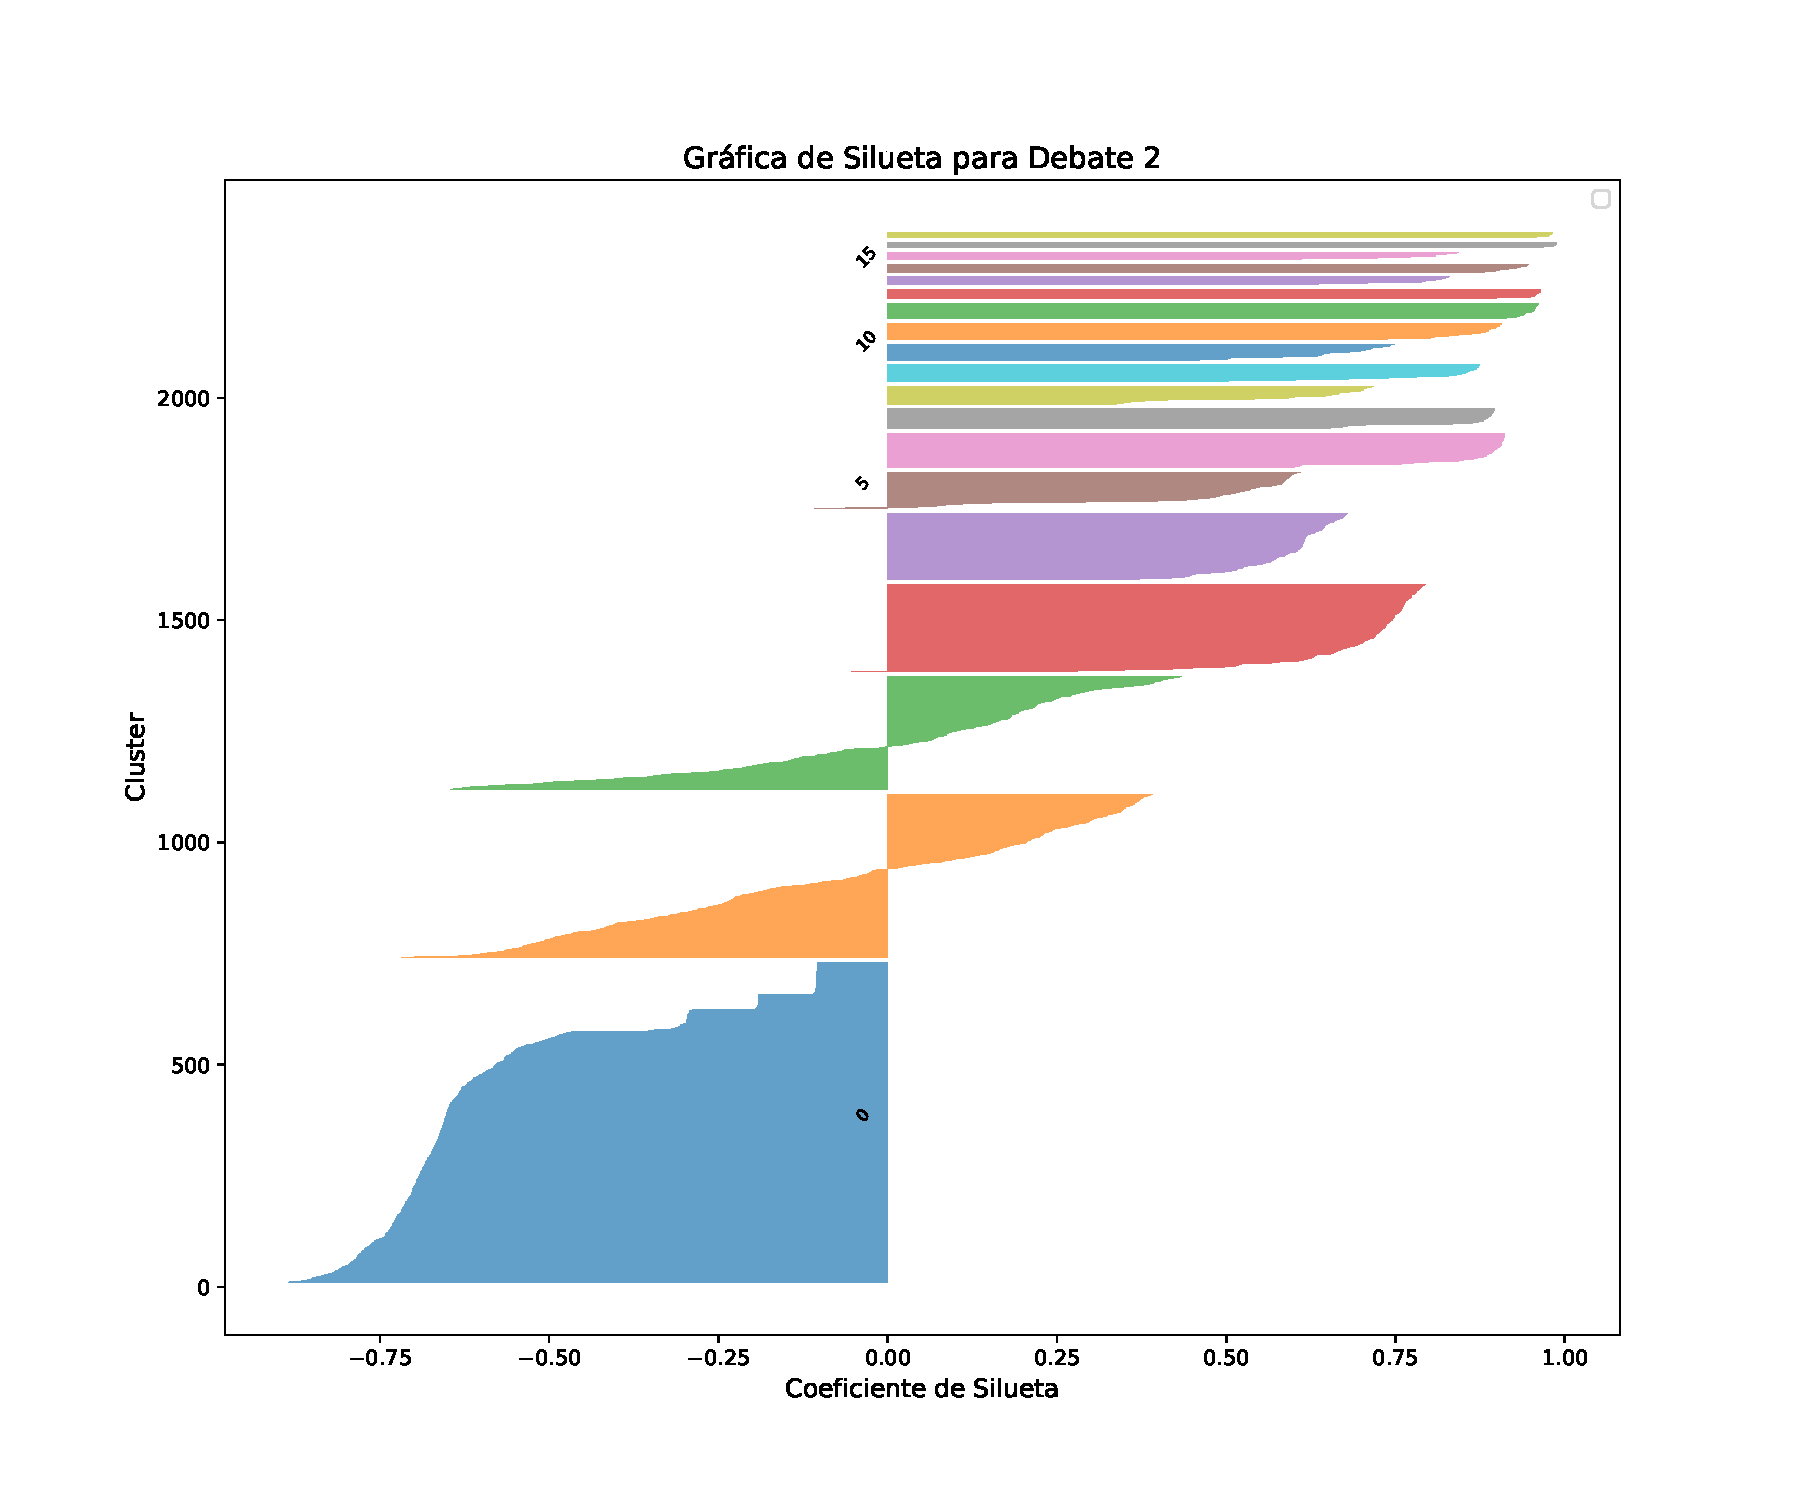
\includegraphics[width=\linewidth]{silhouette_debate2.pdf} 
			\caption{Gráfica de Silueta para el segundo debate}
			\label{fig:silDeb2}
		\end{minipage}
		\hfill % Espacio flexible entre las dos imágenes
		\begin{minipage}{0.49\textwidth}
			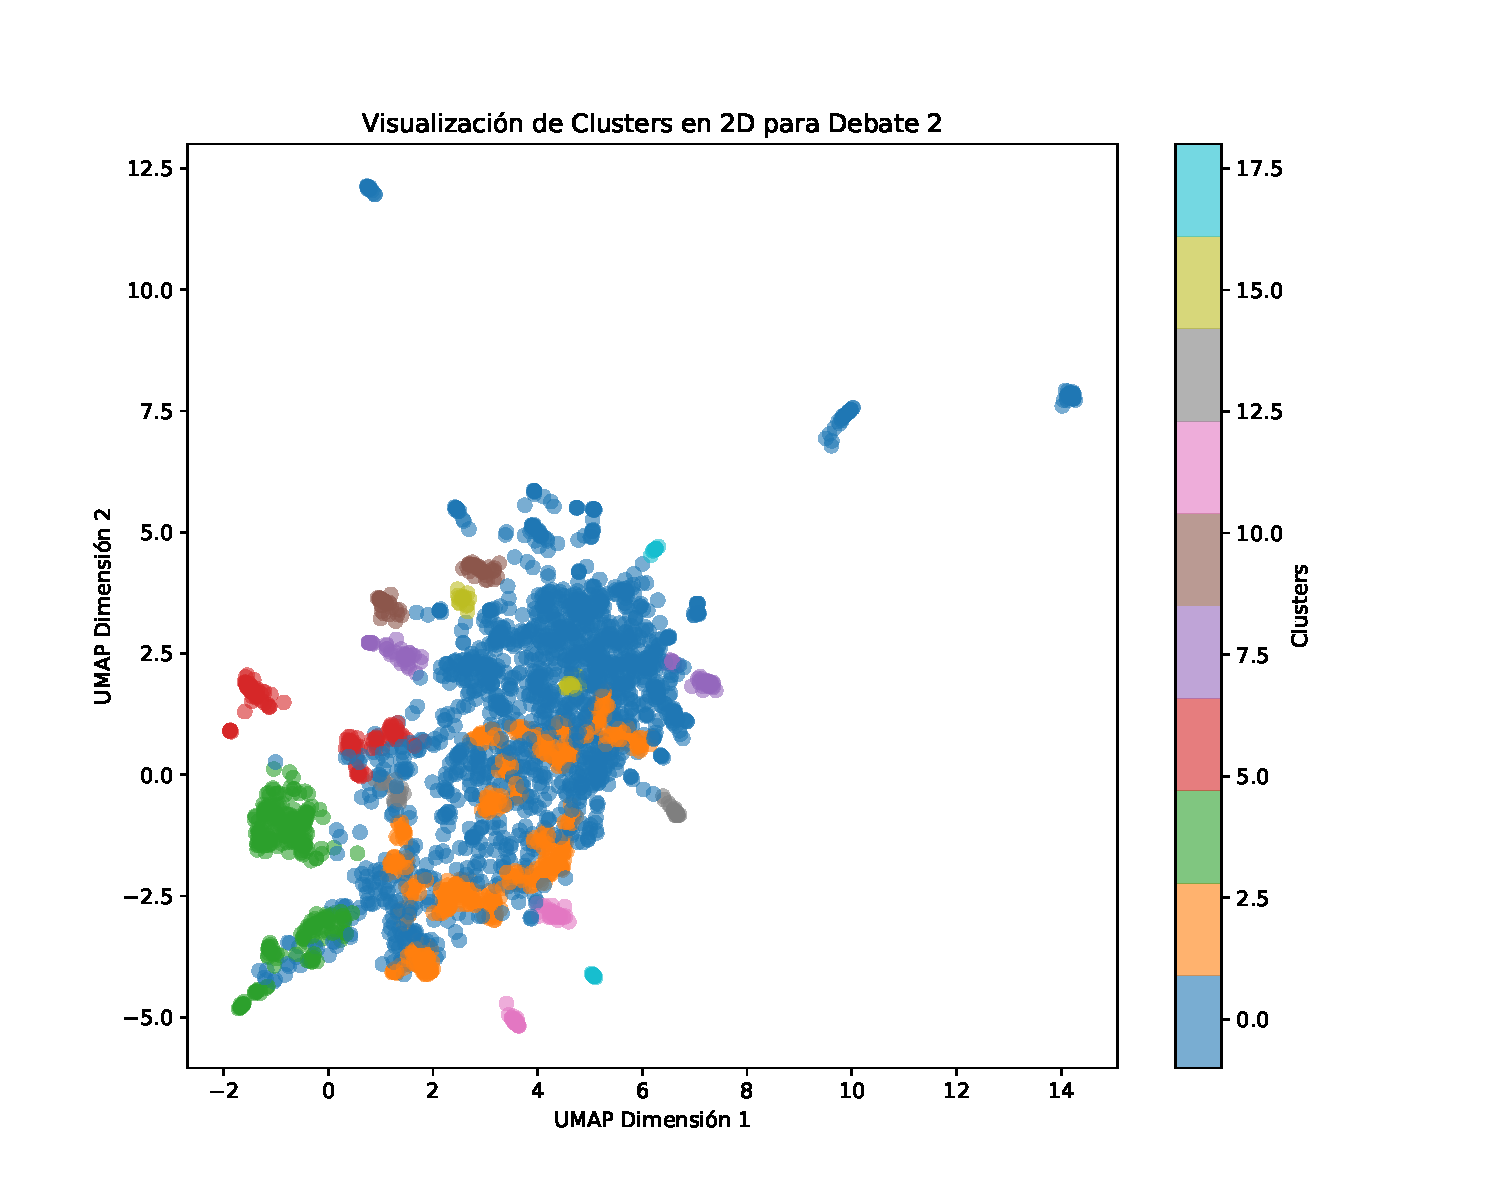
\includegraphics[width=\linewidth]{clusters_debate2.pdf}
			\caption{Grafica de clusters del segundo debate}
			\label{fig:clustDeb2}
		\end{minipage}
	\end{figure}
	
	En la figura \ref{fig:silDeb2}, los resultados muestran menos clusters con coeficientes de silueta negativos en comparación con el Debate 1, lo que sugiere una mejor separación de los temas. Algunos clusters presentan valores significativamente altos, lo que implica la existencia de temas bien definidos y con alta cohesión. No obstante, hay una menor cantidad de clusters grandes en comparación con el Debate 1, lo que puede indicar una mayor fragmentación de los temas discutidos durante este evento.
	
	\vspace{4mm}
	\textbf{Debate 3}

	\begin{figure}[h!]
		\centering
		\begin{minipage}{0.49\textwidth} % Mitad del ancho de la página
			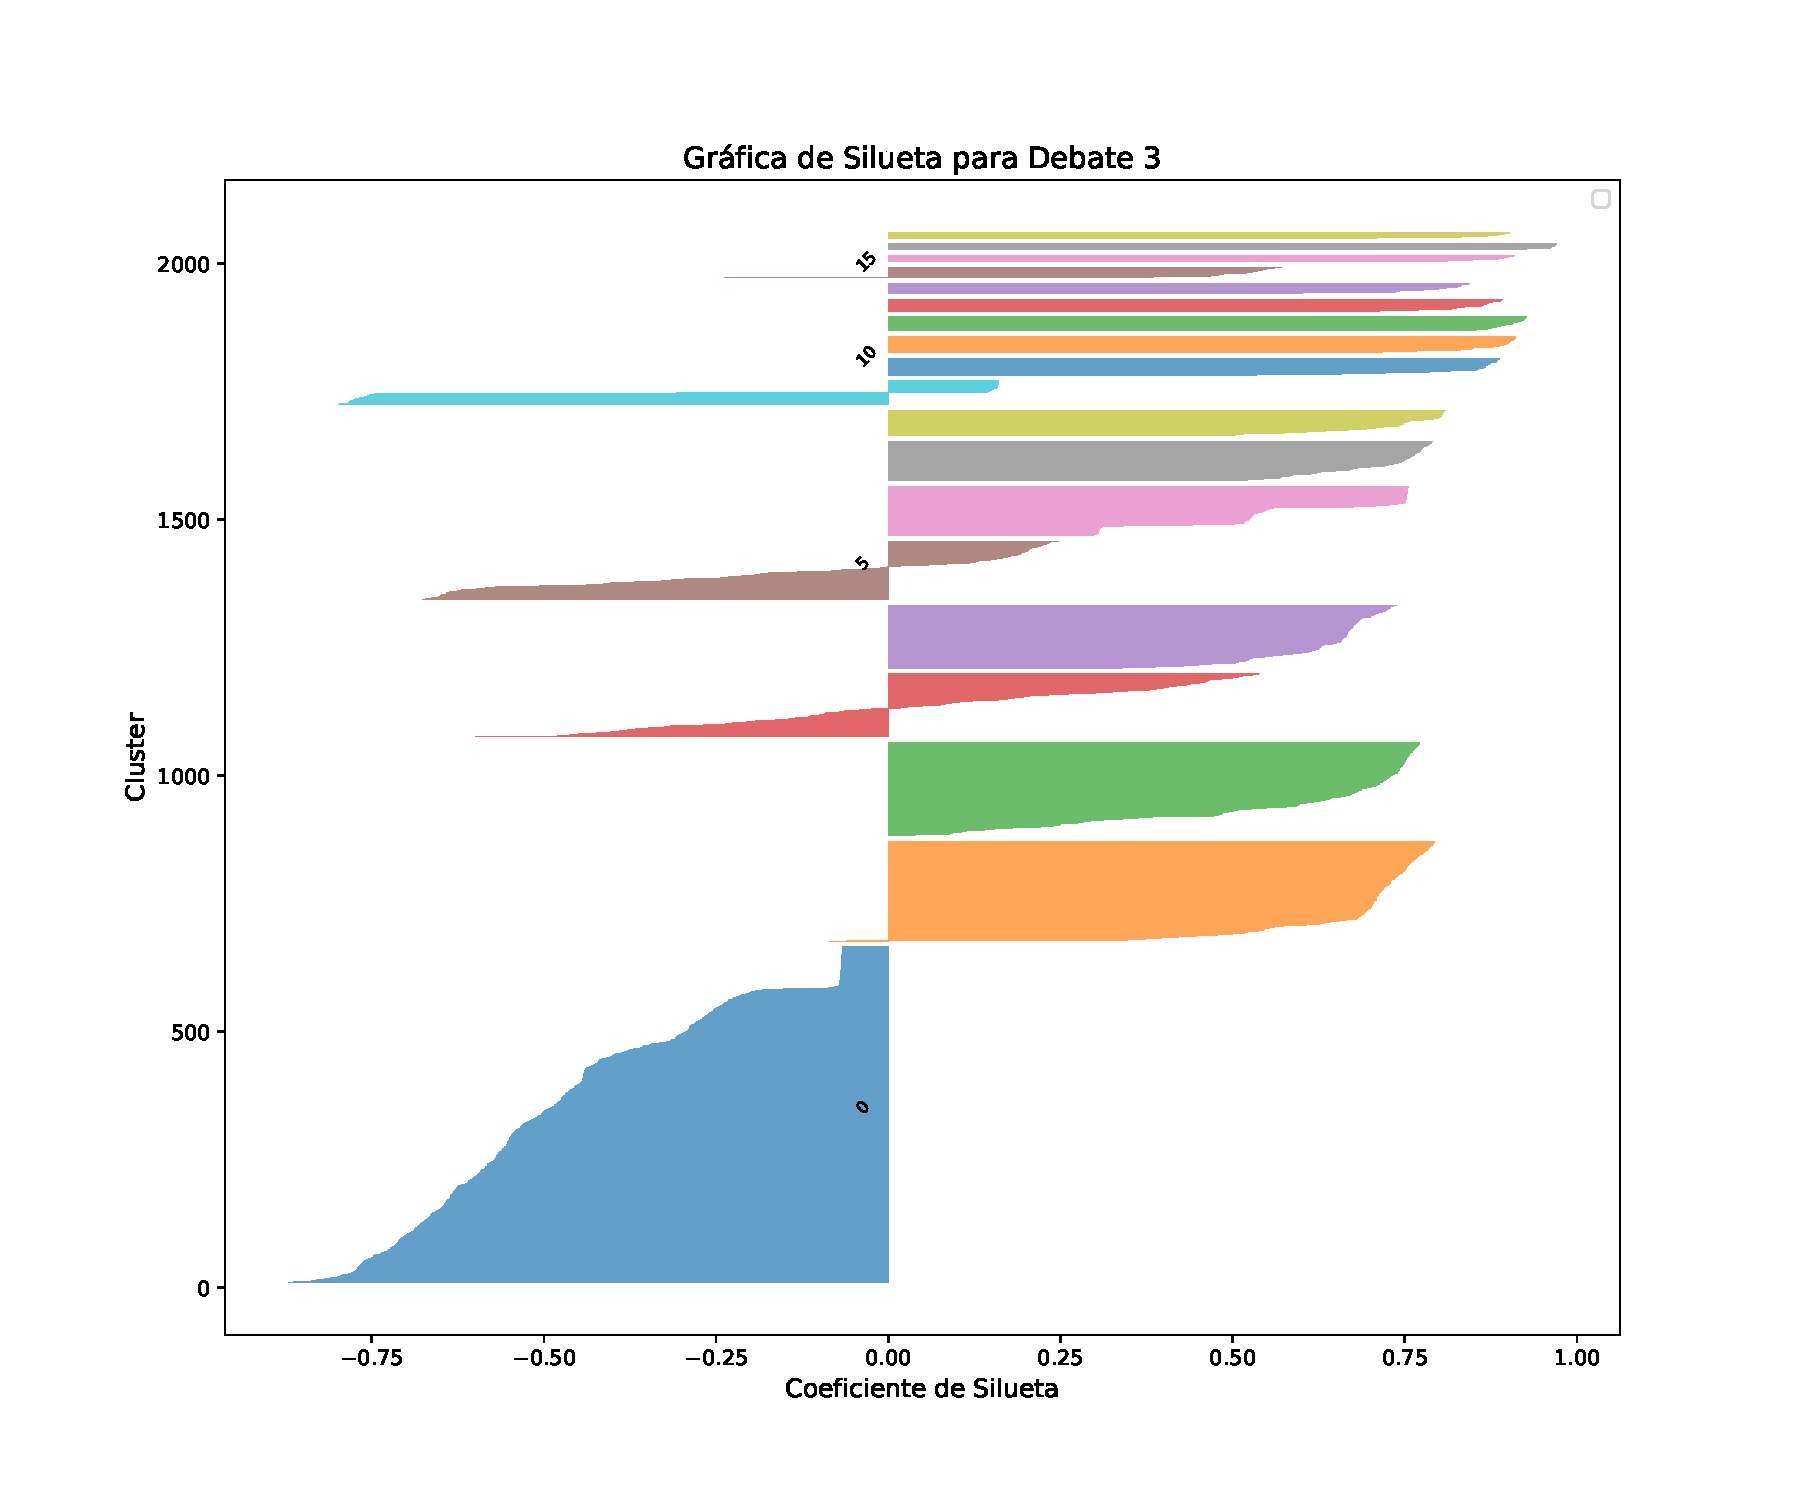
\includegraphics[width=\linewidth]{silhouette_debate3.pdf} 
			\caption{Gráfica de Silueta para el tercer debate}
			\label{fig:silDeb3}
		\end{minipage}
		\hfill % Espacio flexible entre las dos imágenes
		\begin{minipage}{0.49\textwidth}
			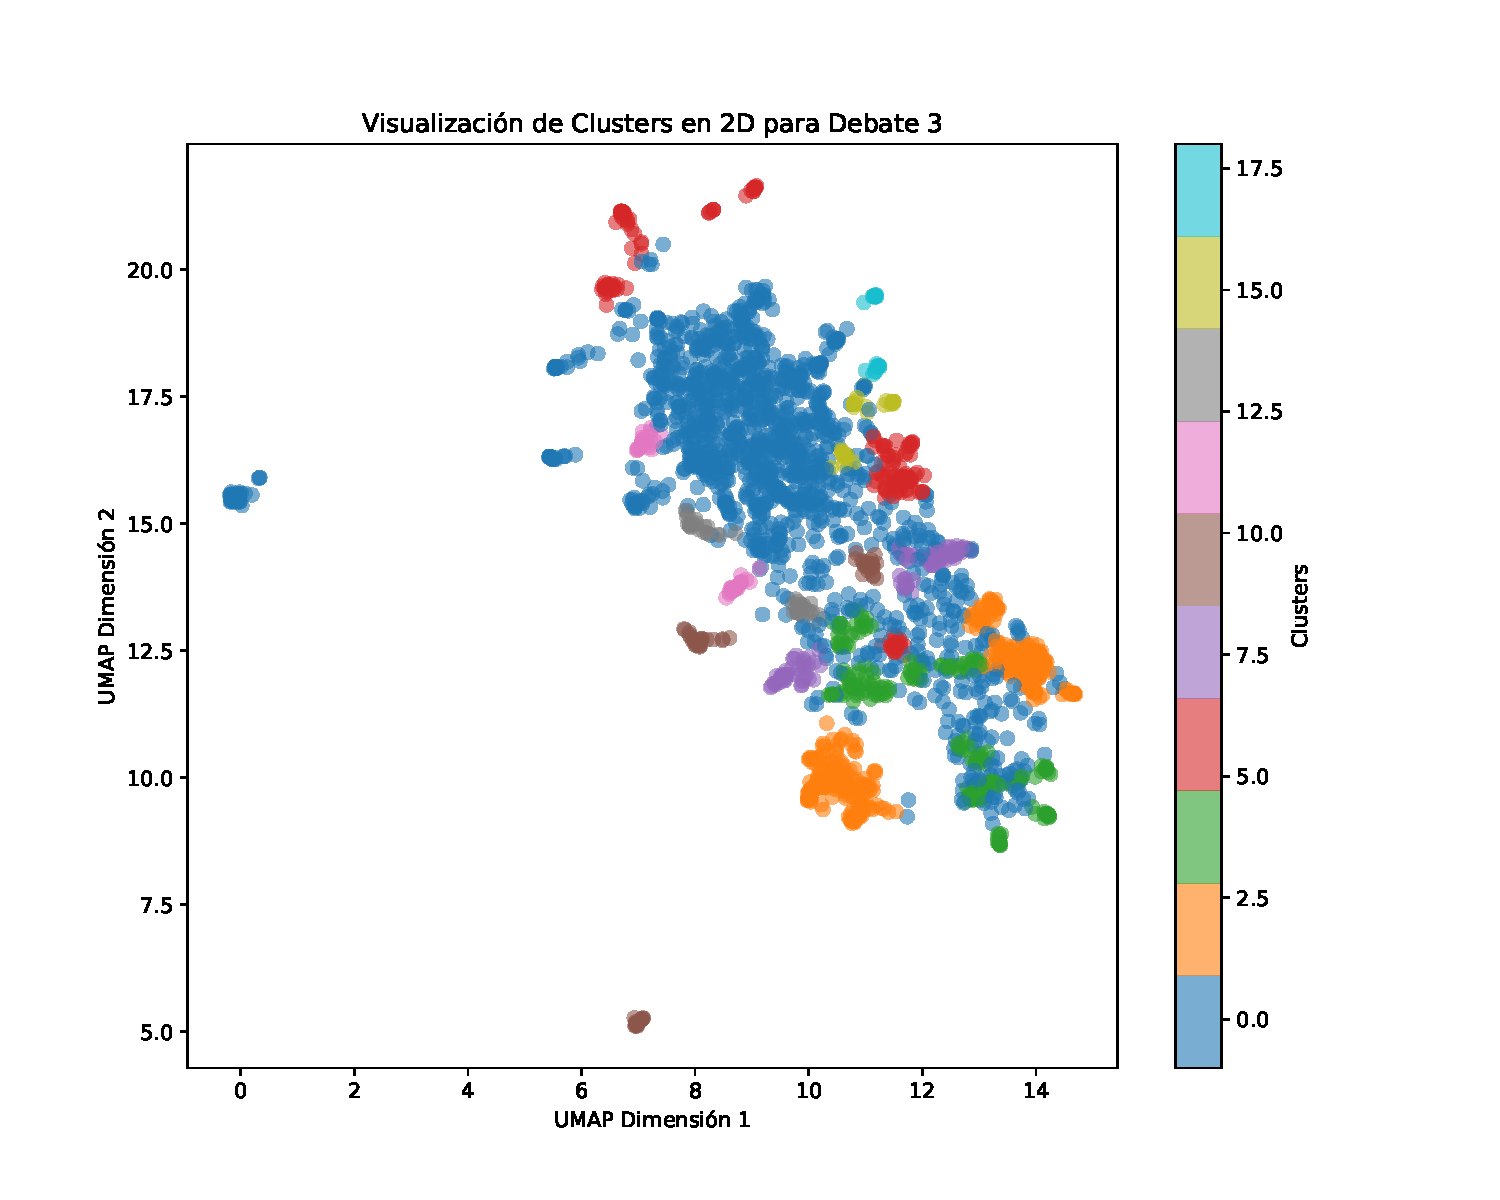
\includegraphics[width=\linewidth]{clusters_debate3.pdf}
			\caption{Grafica de clusters del tercer debate}
			\label{fig:clustDeb3}
		\end{minipage}
	\end{figure}
	
	La gráfica de silueta de la figura \ref{fig:silDeb3} muestra un patrón intermedio entre los dos debates anteriores. Se observa una mayor dispersión en los coeficientes de silueta, con algunos clusters bien definidos (valores altos) y otros con valores cercanos a cero o negativos. Esto sugiere que, aunque hubo temas centrales, también existieron comentarios que no pudieron ser agrupados de manera eficiente, posiblemente debido a una mayor variedad en los tópicos discutidos.
	
	\vspace{4mm}
	\textbf{Día de la Elección}

	\begin{figure}[h!]
		\centering
		\begin{minipage}{0.49\textwidth} % Mitad del ancho de la página
			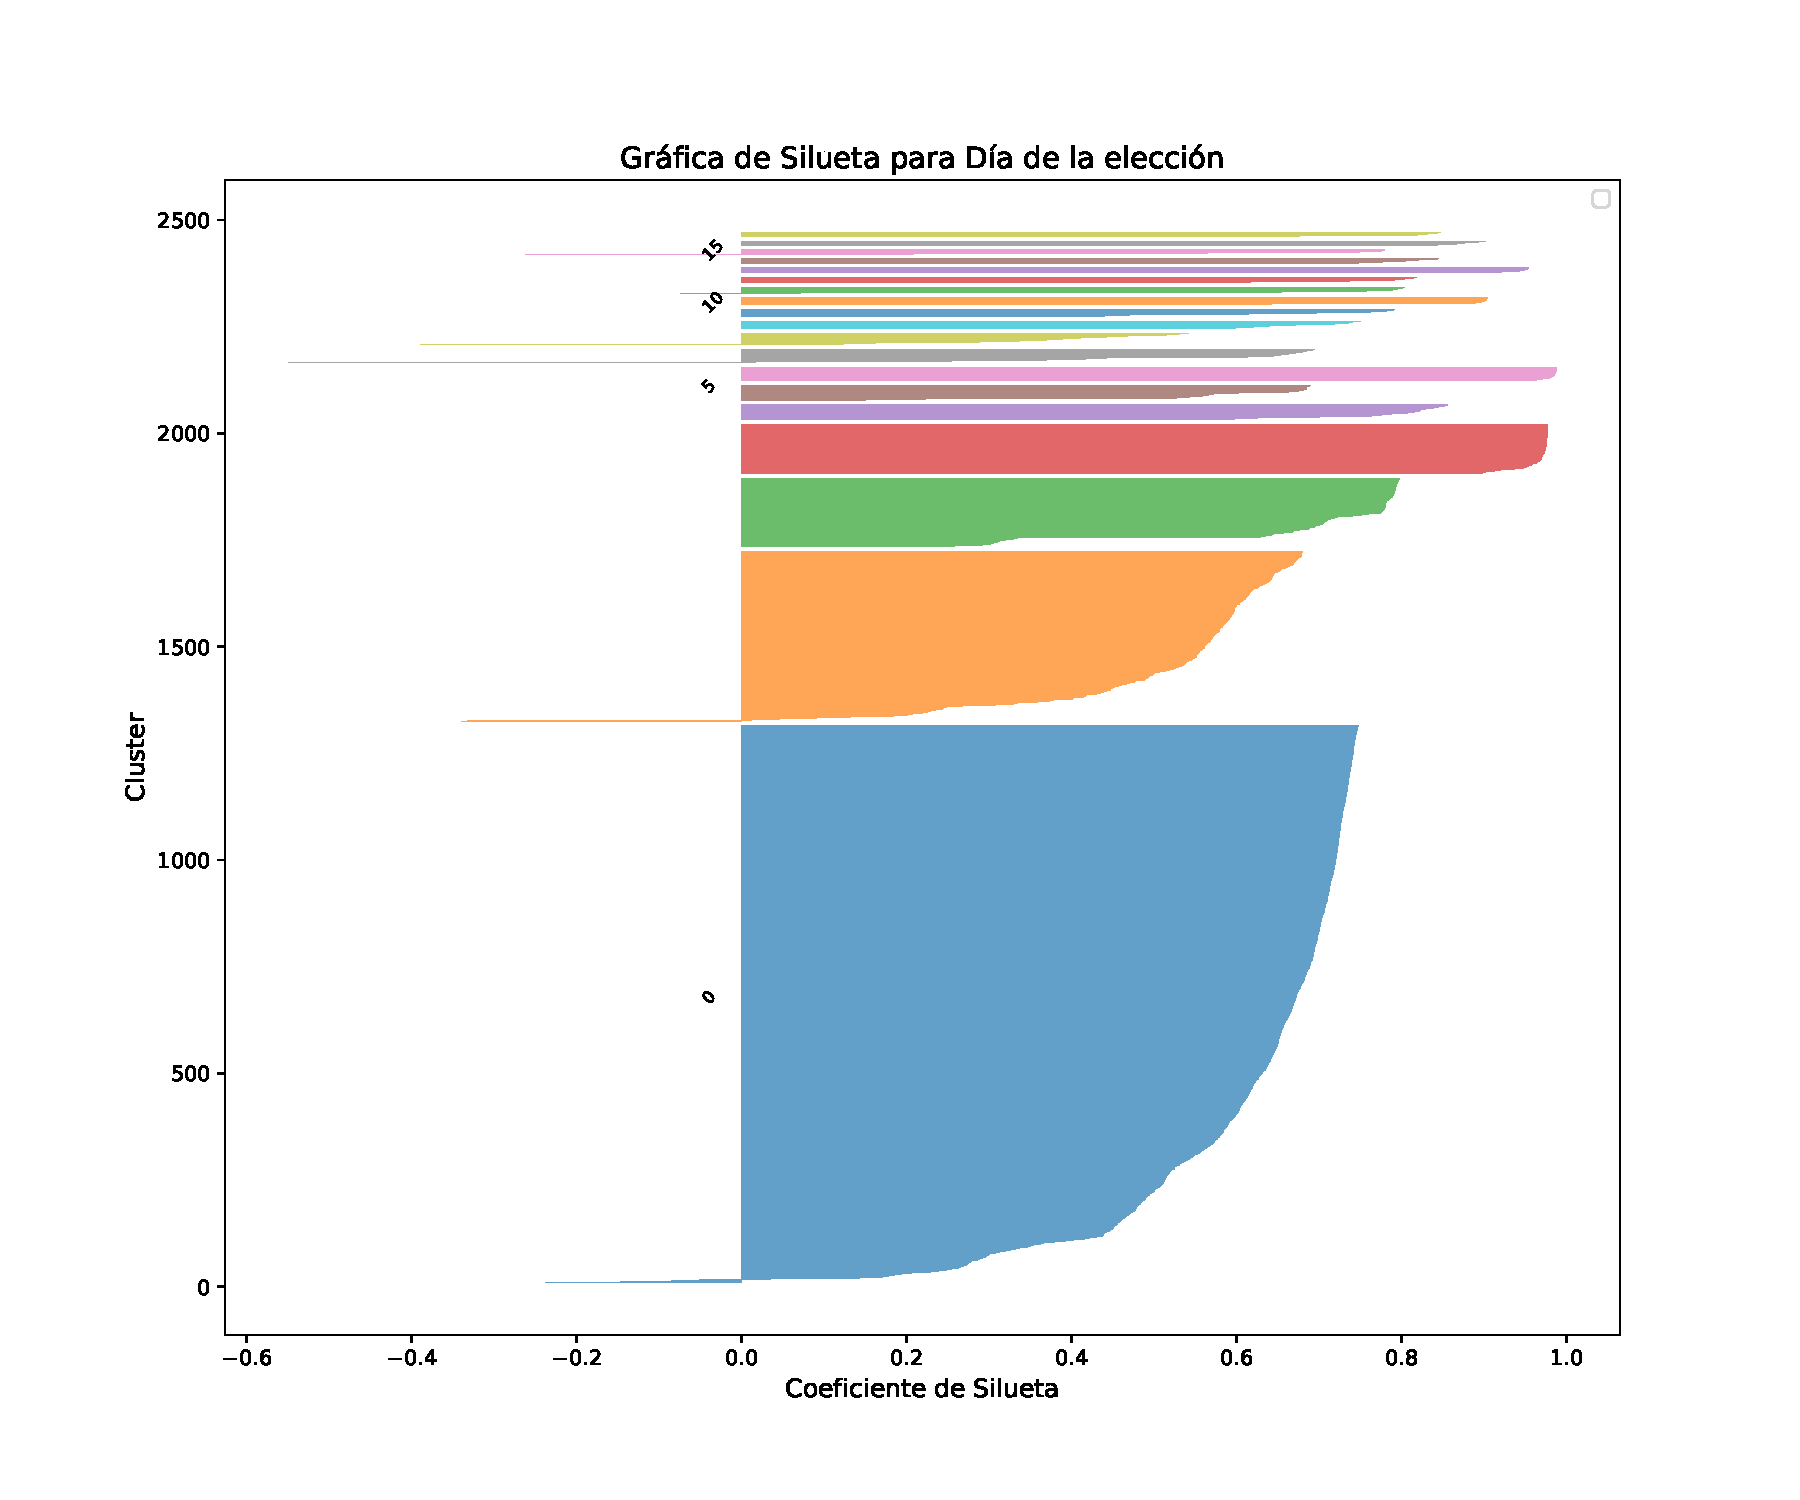
\includegraphics[width=\linewidth]{silhouette_diaEleccion.pdf} 
			\caption{Gráfica de Silueta para el Dia de la Elección}
			\label{fig:silDiaEleccion}
		\end{minipage}
		\hfill % Espacio flexible entre las dos imágenes
		\begin{minipage}{0.49\textwidth}
			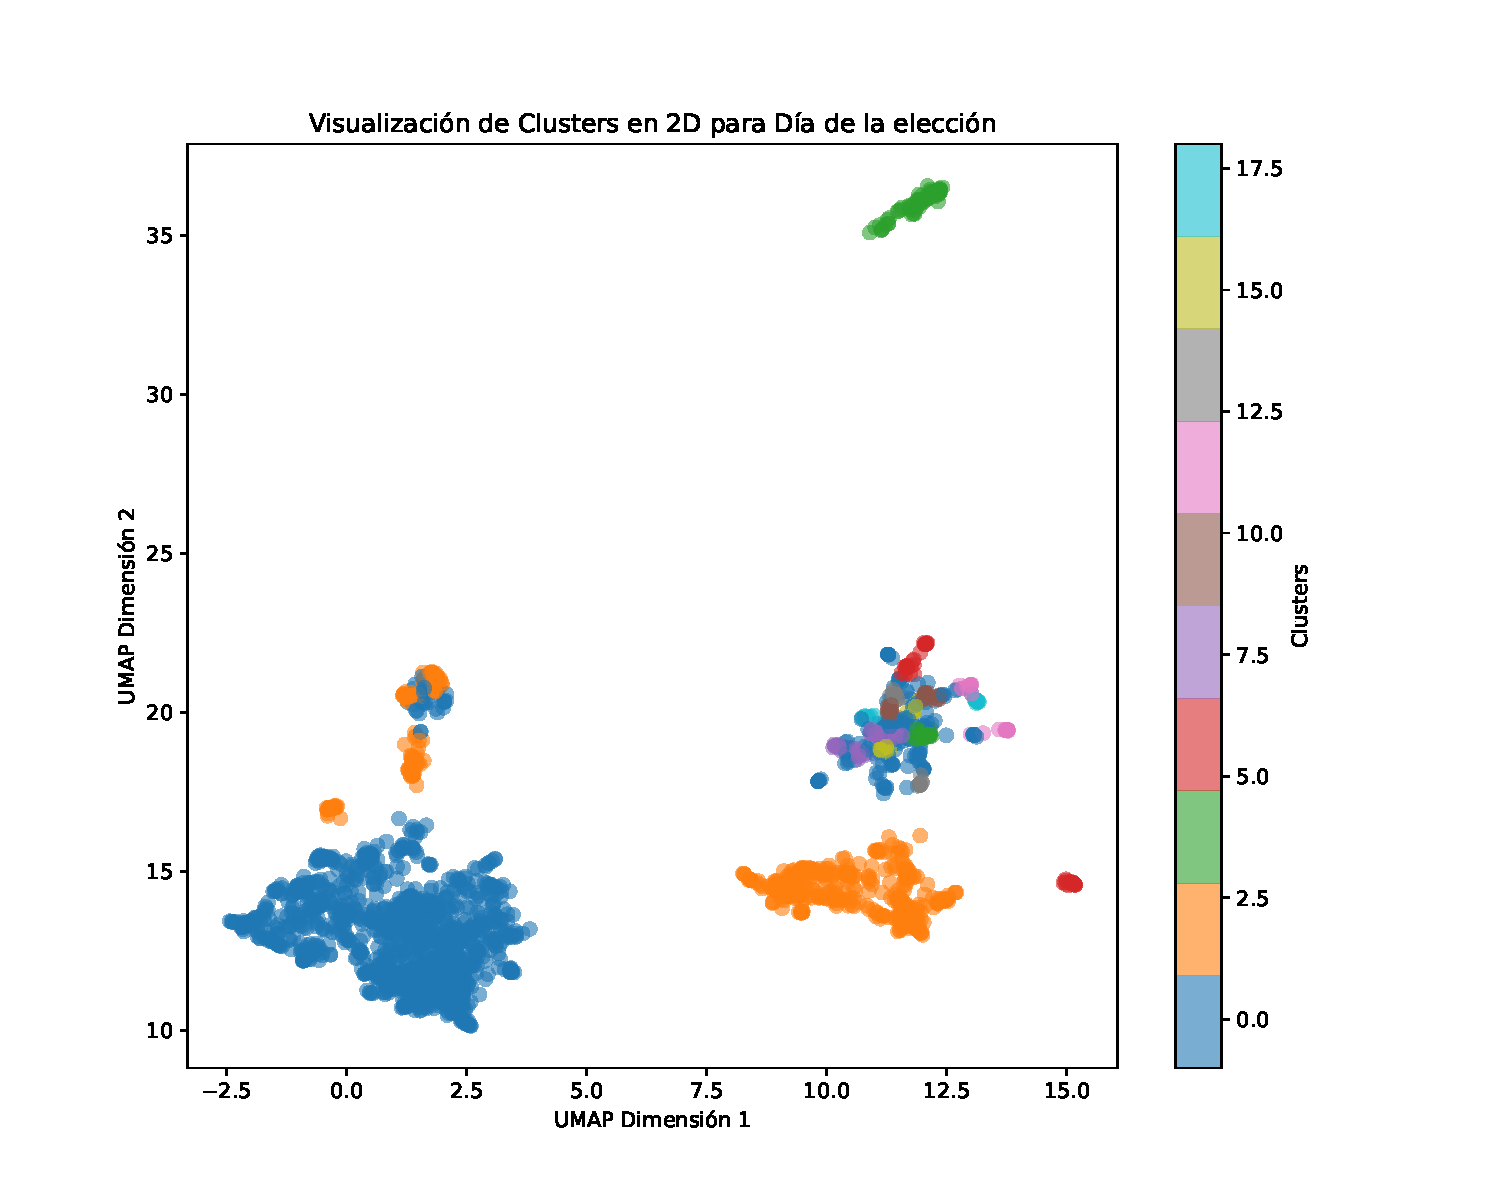
\includegraphics[width=\linewidth]{clusters_diaElección.pdf}
			\caption{Grafica de clusters el Dia de la Elección}
			\label{fig:clustDiaEleccion}
		\end{minipage}
	\end{figure}
	
	En el Día de la Elección, la gráfica de silueta revela una menor cantidad de clusters con coeficientes negativos, lo que indica una mejor cohesión general en comparación con los debates. Esto podría deberse a que los temas discutidos durante este evento fueron más claros y específicos, como resultados, participación ciudadana y reacciones inmediatas. Además, los clusters grandes tienen valores de silueta significativamente altos, lo que sugiere que capturan temas centrales con alta claridad.
	
	En general, las gráficas de silueta indican que los clusters generados tienen una calidad aceptable, especialmente aquellos con valores de silueta superiores a 0.5. Las diferencias entre los eventos reflejan variaciones en la claridad y cohesión de los temas discutidos, siendo el Día de la Elección el evento con mejores resultados en términos de cohesión de clusters.
	
	\subsubsection{Selección de Tópicos Más Populares}
	
	El coeficiente de silueta fue una métrica clave en este estudio, no solo para evaluar la calidad de los clusters generados, sino también para garantizar que los tópicos seleccionados sean representativos de los temas principales discutidos durante el periodo electoral. Este coeficiente mide tanto la cohesión interna de los clusters como su separación respecto a otros. 
	
	Es crucial destacar que si hubiéramos seleccionado temas basándonos únicamente en la cantidad de comentarios asociados, sin considerar el coeficiente de silueta, podríamos haber incluido clusters que, aunque populares, carecen de una estructura bien definida. Dichos clusters podrían reflejar ruido en los datos o discusiones ambiguas, sin un tema central claro. Por el contrario, los temas seleccionados representan las discusiones más destacadas y organizadas en las redes sociales durante los debates y el día de la elección.
	
	Para visualizar esta información, se generó un diagrama de burbuja en el que cada burbuja representa un tópico. El tamaño de la burbuja corresponde al número de comentarios asociados al tema, mientras que su posición en el eje x refleja el coeficiente de silueta promedio.
	
	\begin{figure}[H]
		\centering
		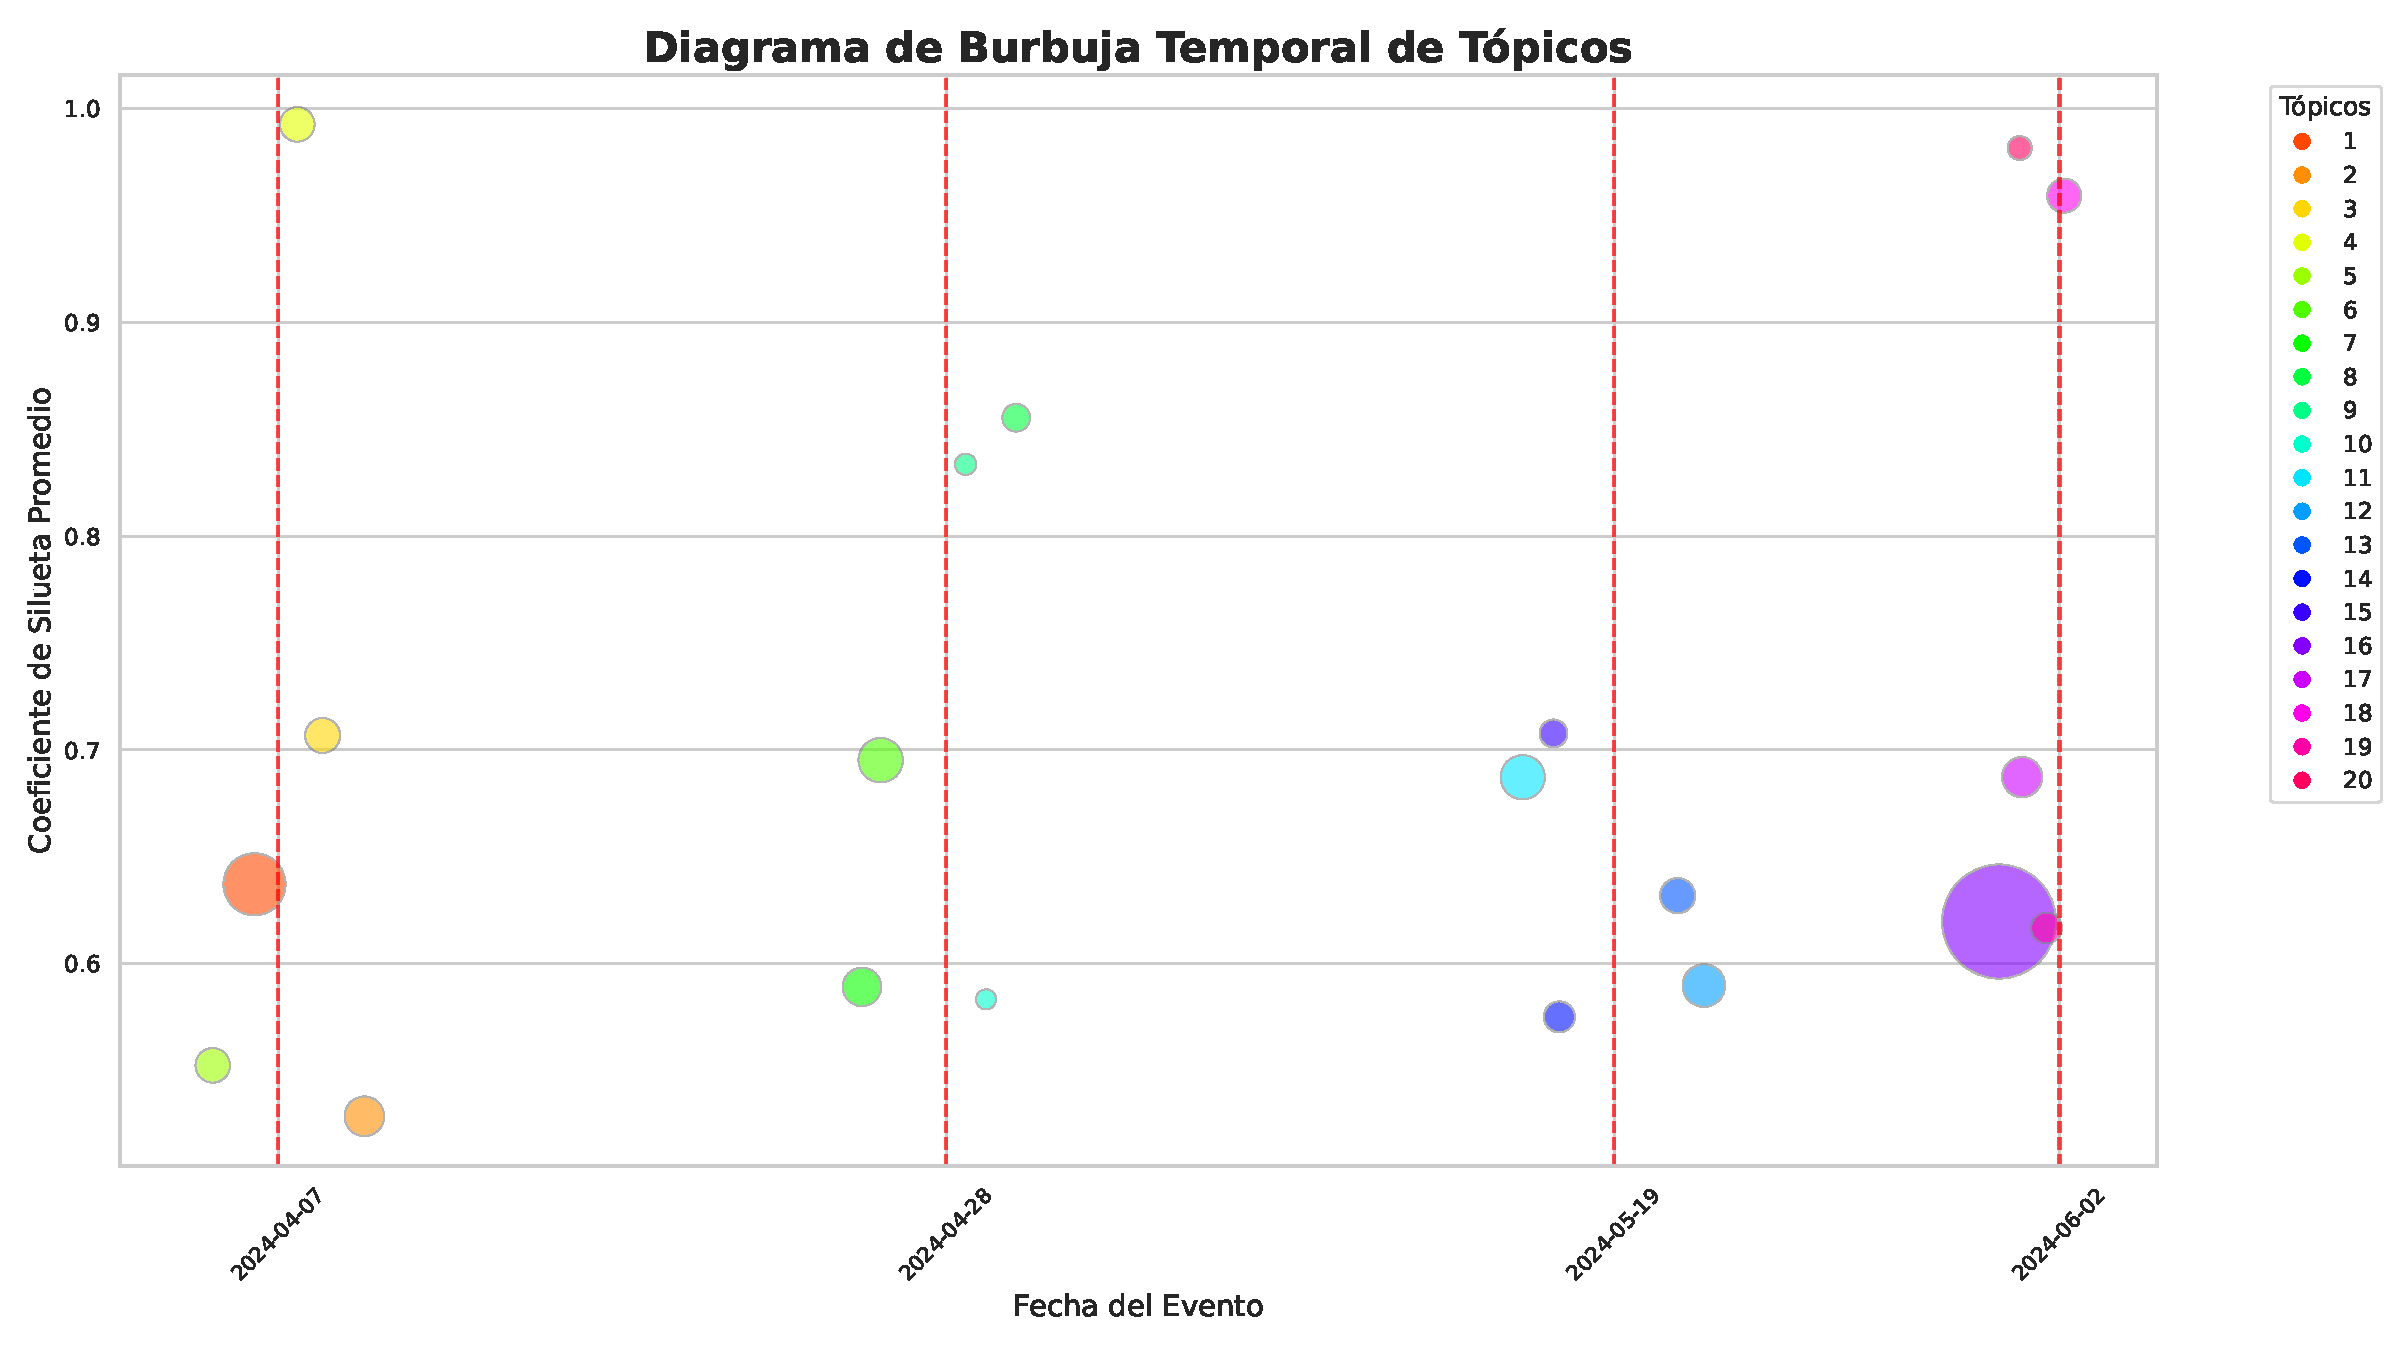
\includegraphics[width=0.85\textwidth]{diagrama_burbuja.pdf}
		\caption{Diagrama de burbuja de los tópicos más populares}
		\label{fig:diagrama_burbuja}
	\end{figure}
	\vspace{-5mm}
	\begin{table}[H]
		\centering
		\begin{tabular}{|l|l|l|r|l|c|}
			\hline
			\textbf{Num} & \textbf{Evento} & \textbf{Fecha} & \textbf{Tópico} & \textbf{Cantidad} & \textbf{Silhouette Promedio} \\
			\hline
			1 & Debate 1 & 2024-04-07 & debate, voto, candidatos, votar & 389 & 0.637 \\
			2 & Debate 1 & 2024-04-07 & preguntas, xochitl, mentiras, vergüenza & 158 & 0.528 \\
			3 & Debate 1 & 2024-04-07 & educación, niños, escuelas, escuela & 123 & 0.706 \\
			4 & Debate 1 & 2024-04-07 & tiempo, minuto, quitan, reloj & 121 & 0.992 \\
			5 & Debate 1 & 2024-04-07 & presidenta, presidente, maynez, claudia & 120 & 0.552 \\
			6 & Debate 2 & 2024-04-28 & méxico, mexicanos, mexico, presidente & 198 & 0.695 \\
			7 & Debate 2 & 2024-04-28 & presidenta, presidente, claudia, sheinbaum & 149 & 0.589 \\
			8 & Debate 2 & 2024-04-28 & gasolina, subio, unidos, precio & 77 & 0.855 \\
			9 & Debate 2 & 2024-04-28 & jajaja, jajajaja, PAN, xochitl & 46 & 0.833 \\
			10 & Debate 2 & 2024-04-28 & doctora, vamos, plan, c & 41 & 0.583 \\
			11 & Debate 3 & 2024-05-19 & méxico, mexicanos, mexico, hacer & 196 & 0.687 \\
			12 & Debate 3 & 2024-05-19 & voto, votar, candidata, xochitl & 183 & 0.589 \\
			13 & Debate 3 & 2024-05-19 & presidenta, presidente, claudia, xochitl & 124 & 0.631 \\
			14 & Debate 3 & 2024-05-19 & sheinbaum, claudia, maynez, viva & 97 & 0.575 \\
			15 & Debate 3 & 2024-05-19 & debate, no, preguntas, propuestas & 78 & 0.707 \\
			16 & Día Elección & 2024-06-02 & méxico, elecciones, claudia, presidenta & 1306 & 0.619 \\
			17 & Día Elección & 2024-06-02 & siguiente, presidenta, claudia, méxico & 162 & 0.687 \\
			18 & Día Elección & 2024-06-02 & voté, xochitl, representado, pri & 117 & 0.959 \\
			19 & Día Elección & 2024-06-02 & urnas, vota, inundemos, votar & 95 & 0.616 \\
			20 & Día Elección & 2024-06-02 & mexico, voté, xochitl, presidenta & 58 & 0.981 \\
			\hline
		\end{tabular}
		\caption{Tópicos populares durante los debates y el día de la elección}
		\label{tab:topicos_seleccionados}
	\end{table}
	
	\subsubsection{Comparación de los Temas Discutidos}
	
	El análisis muestra claras diferencias entre los temas discutidos en los debates y el día de la elección, reflejando cómo cambia el interés ciudadano a lo largo del proceso electoral.
	
	Durante los debates, las conversaciones se centraron en evaluar las propuestas de los candidatos y su desempeño. Los usuarios discutieron temas como educación, economía y recursos energéticos, mientras que aspectos como el manejo del tiempo y las declaraciones polémicas también generaron opiniones divididas. Este periodo fue más analítico, con un enfoque en las ideas presentadas y su posible impacto.
	
	En contraste, el día de la elección, las discusiones giraron principalmente en torno a los resultados preliminares y las experiencias de los votantes. Las menciones a Claudia Sheinbaum dominaron las conversaciones, mientras que muchos ciudadanos compartieron sus razones para votar y reflexionaron sobre el proceso electoral, destacando un tono más emocional y participativo.
	
	Mientras que los debates promovieron un análisis crítico de las propuestas, el día de la elección estuvo marcado por la reacción inmediata a los resultados y la experiencia personal de los votantes. Este cambio evidencia cómo las prioridades de los ciudadanos evolucionan desde lo conceptual hacia lo concreto a medida que avanza el proceso electoral.
	
	\subsection{Reconstrucción de la Narrativa Política en Redes Sociales}
	
	A lo largo del proceso electoral, las redes sociales se convirtieron en un espejo de las emociones y preocupaciones de los ciudadanos. Los debates presidenciales y el día de la elección fueron escenarios digitales donde el electorado discutió, reflexionó y compartió sus opiniones, dejando entrever las dinámicas políticas y sociales que definieron esta jornada histórica. La narrativa construida en estas plataformas no solo refleja lo que los ciudadanos pensaban sobre los candidatos, sino también qué temas les importaban y cómo estos influían en sus percepciones.
	
	\subsubsection{Narrativa durante los Debates Presidenciales}
	
	Los debates presidenciales fueron el punto de partida para que las audiencias empezaran a formar y compartir sus opiniones. Durante el primer debate, las discusiones giraron en torno a las propuestas de los candidatos y en las fallas tecnicas del debate, con un interés particular en temas como la educación y el bienestar social. Claudia Sheinbaum logró captar la atención como una candidata confiable, generando comentarios que mostraban interés en lo que proponía. Sin embargo, esta posición equilibrada contrastaba con las reacciones hacia Xóchitl Gálvez, quien se enfrentó a críticas por la solidez de sus argumentos, lo que polarizó las opiniones a su alrededor. Por otro lado, Jorge Álvarez Maynez parecía pasar desapercibido; aunque presente en las discusiones, su participación no despertó emociones significativas ni discusiones intensas.
	
	En el segundo debate, el enfoque de las conversaciones cambió. Los temas económicos, como el manejo del presupuesto y los precios de los recursos básicos, dominaron las discusiones. La audiencia parecía más interesada en los problemas del día a día, y esto se reflejó en un tono más crítico hacia el gobierno actual. 	A pesar de ello, Claudia Sheinbaum mantuvo su posición como una figura sólida, resaltando propuestas como el \textit{Plan C}, e incluso, se hablaba fuertemente de que seria la siguiente presidenta de México, mientras que Gálvez continuó enfrentando polarización, navegando entre aquellos que se burlaban de ella y quienes tenían expectativa en que se pondría la banda presidencial. Álvarez Maynez, aunque nuevamente menos discutido, comenzó a despertar cierta curiosidad, aunque sin generar las emociones polarizantes de sus contrincantes.
	
	El tercer debate presentó una dinámica más definida. Los usuarios no solo escuchaban a los candidatos, sino que hicieron énfasis en que los candidatos no estaban presentando propuestas ni respondiendo a las preguntas, ademas se sembró un sentimiento patriótico en sus opiniones. Los comentarios sobre Sheinbaum destacaron su capacidad de inspirar confianza en una parte significativa del electorado, consolidando su imagen como una figura fuerte. En contraste, Gálvez seguía siendo objeto de intensas discusiones, con una clara división entre quienes la apoyaban y quienes la criticaban. Álvarez Maynez, por su parte, permaneció en el margen de las conversaciones, con pocos comentarios apasionados sobre su desempeño, lo que reforzó la idea de que no estaba logrando conectar emocionalmente con la audiencia.
	
	\subsubsection{Narrativa durante el Día de la Elección}
	
	El día de la elección trajo consigo un cambio en el tono y enfoque de las conversaciones. Desde las primeras horas, los usuarios compartieron sus emoción por acudir a las urnas, narrando principalmente su entusiasmo de que su candidata Claudia o Xochitl ocupara la silla presidencial. Las discusiones estuvieron marcadas por una mezcla de optimismo y ansiedad mientras los ciudadanos esperaban los primeros resultados preliminares.
	
	Claudia Sheinbaum estaba en gran parte de las conversaciones durante la mañana, con mensajes que destacaban su liderazgo y generaban una sensación de confianza entre sus seguidores. En contraste, Xóchitl Gálvez domino la conversación y despertó una mezcla de emociones: sus simpatizantes la defendían con pasión, mientras que otros se mantenían críticos hacia su candidatura, lo que reflejaba el tono polarizado que la había acompañado desde los debates. Mientras tanto, Jorge Álvarez Maynez seguía siendo una figura poco discutida, casi ausente en las emociones más intensas del día.
	
	Conforme avanzaba el día, las emociones comenzaban a estabilizarse. Los usuarios discutían temas relacionados con la organización del proceso electoral y reflexionaban sobre los posibles resultados de la jornada. Por la tarde, las menciones hacia Sheinbaum se centraron en consolidar su imagen como una figura capaz de liderar, mientras que Gálvez seguía generando respuestas divididas, destacando la controversia que su candidatura provocaba. Álvarez Maynez, por otro lado, parecía ser un espectador más de la jornada, con pocos comentarios que mostraran entusiasmo o rechazo hacia su figura.
	
	Al caer la noche, la narrativa alcanzó su punto culminante. Los resultados preliminares comenzaron a circular, y las redes sociales se llenaron de reacciones inmediatas. Sheinbaum se posicionó como la protagonista de la conversación, con un aumento en los mensajes positivos que celebraban su posible victoria. Gálvez, aunque todavía presente en las discusiones, enfrentó un incremento en las críticas y una disminicion en su apoyo, lo que reflejaba una percepción menos favorable hacia el final del día. En cuanto a Álvarez Maynez, su participación en las conversaciones continuó siendo marginal, consolidándolo como el candidato menos influyente en la narrativa digital.
	
	\subsubsection{Evolución de la Narrativa y su Significado}
	
	La narrativa política en redes sociales durante esta jornada electoral muestra cómo las emociones y prioridades del electorado evolucionaron en función de los eventos. Durante los debates, las discusiones estuvieron marcadas por un análisis crítico de las propuestas y el desempeño de los candidatos, mientras que el día de la elección trajo consigo una dimensión más emocional y participativa, enfocada en las experiencias personales y los resultados.
	
	Los temas discutidos no solo reflejan las preocupaciones de los ciudadanos, sino también las dinámicas sociales que definen el diálogo político en entornos digitales. La educación, la economía y el bienestar social dominaron los debates, mientras que el día de la elección estuvo marcado por un interés en los resultados y una celebración del acto democrático. Este análisis destaca cómo las redes sociales se han convertido en un espacio central para que los ciudadanos expresen sus emociones, reflexionen sobre las propuestas y participen en la construcción de una narrativa colectiva en torno al proceso electoral.
	
	
	
	\section{Conclusiones}
	
	El estudio de minería de textos llevado a cabo sobre los debates presidenciales y el día de la elección presidencial en México 2024 permite extraer conclusiones clave que combinan análisis de sentimientos y modelado de tópicos, arrojando una visión integral de cómo la percepción pública evolucionó durante el proceso electoral.
	
	\subsection{Dinámica de los Debates Presidenciales}
	Los debates presidenciales evidenciaron las diferencias en cómo los candidatos fueron percibidos por la ciudadanía, con los tópicos discutidos marcando el tono de las emociones reflejadas en los comentarios:
	\begin{itemize}
		\item Claudia Sheinbaum se consolidó como una figura de balance entre emociones positivas y neutras. Los comentarios destacaban su perfil presidencial, respaldado por temas relacionados con su liderazgo, como \textit{México}, \textit{presidenta} y \textit{futuro}. Esto sugiere que su discurso conectó con las expectativas de los votantes, posicionándola como una candidata sólida y confiable.
		\item La polarización de Xóchitl Gálvez, quien continuó enfrentando críticas siendo etiquetada en tópicos como \textit{mentirosa} y \textit{sin vergüenza}. Además, los comentarios humorísticos y descalificaciones fueron recurrentes, como se reflejó en tópicos que incluían términos como \textit{mentiras}, \textit{vergüenza} y expresiones de burla (\textit{jajaja}). Esto muestra cómo ciertos segmentos del electorado percibieron su desempeño como polarizador y poco convincente.
		\item Jorge Álvarez Maynez mantuvo una neutralidad abrumadora, reflejada en su falta de mención en temas destacados. Esto sugiere que, si bien no polarizó opiniones, tampoco logró generar un impacto significativo en la audiencia, quedando al margen de las conversaciones clave del proceso.
	\end{itemize}
	En general, los debates presidenciales se caracterizaron por un electorado crítico y atento, evaluando tanto los argumentos de los candidatos como su desempeño en tiempo real.
	
	\subsection{El Día de la Elección: Resultados y Participación Ciudadana}
	El día de la elección marcó un cambio de enfoque, donde las emociones y los tópicos discutidos se centraron en los resultados y las experiencias de los votantes. Esto se reflejó en:
	\begin{itemize}
		\item Claudia Sheinbaum emergió como el centro de las conversaciones, con términos recurrentes como \textit{elecciones}, \textit{Claudia} y \textit{presidenta}, lo que sugiere que muchos usuarios ya la visualizaban como la ganadora. Este cambio hacia un tono predominantemente positivo refuerza la percepción de que su figura generó confianza en gran parte del electorado.
		\item Xóchitl Gálvez continuó enfrentando críticas, aunque sus simpatizantes también expresaron apoyo en términos como \textit{voté por Xóchitl} y \textit{siguiente presidenta}. Sin embargo, la polarización siguió siendo evidente, con una mezcla de comentarios que cuestionaban su autenticidad y otros que celebraban su candidatura.
		\item Jorge Álvarez Maynez se mantuvo en un segundo plano, con menciones mínimas en los tópicos relacionados con la votación. Este patrón refuerza la idea de que su campaña no logró conectar con la audiencia de manera significativa durante el proceso electoral.
	\end{itemize}
	
	Además, los usuarios utilizaron las redes sociales como un espacio para compartir sus experiencias personales de votación, lo que evidencia el papel de estas plataformas como un canal de participación y reflexión ciudadana.
		
	
	\subsection{Implicaciones Generales}
	
	La combinación de análisis de sentimientos y análisis de tópicos permitió capturar no solo los temas más discutidos, sino también las emociones que estos generaron. Este enfoque reveló cómo los ciudadanos reaccionaron de manera diferente en cada etapa del proceso electoral, proporcionando una visión integral de la percepción pública.
	
	Este estudio demuestra cómo las redes sociales actúan como un barómetro del sentir ciudadano en tiempo real, reflejando tanto las emociones como los temas clave del proceso electoral. Los resultados sugieren que los candidatos no solo deben considerar las propuestas que presentan, sino también cómo estas se discuten y perciben en el ámbito digital.
	
	En última instancia, la combinación de análisis de sentimientos y tópicos proporciona una herramienta poderosa para entender las dinámicas de percepción pública, ayudando a identificar los factores que influyen en la narrativa electoral y, potencialmente, en los resultados finales de una elección.
	
	
	
	
	\newpage
	\printbibliography
	
	
	
\end{document}